
% manual maniFEM

\def\version{20.03}

\magnification\magstep1
\nopagenumbers
\pretolerance=1200
\overfullrule=0pt 
\spaceskip=0.3333em plus 1.5pt minus 0.3pt
\xspaceskip=0.5em plus 2pt minus 0.5pt

% Plain TeX interface to psfrag.
% David Carlisle
\input miniltx
\makeatletter
\ifx\@compatibilitytrue\@undefined
  \csname newif\expandafter\endcsname
       \csname if@compatibility\endcsname
\fi
\ifx\raisebox\@undefined
\def\raisebox#1#2{{%
  \setbox0=\hbox{#2}\def\depth{\dp0}\leavevmode\raise#1\box\z@}}
\fi
\ifx\@@underline\@undefined
\let\@@underline\underline
\def\underline{%
  \ifmmode\expandafter\@@underline\else\expandafter\underbar\fi}
\fi
\ifx\sbox\@undefined
\def\sbox#1{\setbox#1\hbox}
\fi
% psfrag loads the core graphics package, but only the extended
% graphicx interface is available from plain TeX so just intercept
% the call and ask for graphicx.
\let\savedRP\RequirePackage
\def\RequirePackage#1{%
  \let\RequirePackage\savedRP
  \ifx\includegraphics\@undefined
  \input graphicx\fi\relax}
\input psfrag.sty
\ifx\pfg@dp\@undefined
\csname newdimen\endcsname\pfg@dp
\csname newdimen\endcsname\pfg@wd
\csname newdimen\endcsname\pfg@dx
\csname newdimen\endcsname\pfg@dy
\fi
\resetatcatcode
% end of interface to psfrag

\def\parbox#1{% \long\def\parbox
  \leavevmode
  \vtop{%
    \hsize0.95\hsize % Pick your size here
    \parindent0pt %
    \parskip\baselineskip
    \sloppy
    #1\par
  }%
}
\def\sloppy{%
  \tolerance 9999 %
  \emergencystretch 3em %
  \hfuzz 0.5pt %
  \vfuzz \hfuzz
}

\font\titlefont=cmr10 at 20pt
\font\sectfont=cmr10 at 14pt
\font\parfont=cmr10 at 12pt
\font\codett=cmtt10 at 9pt
\font\ftntfont=cmr10 at 8pt
\font\ftnttt=cmtt10 at 7pt
\def\section#1{\vfil\eject\centerline{\sectfont #1}\bigskip\bigskip}
\def\paragraph#1{\bigskip\line{\parfont #1\hfil}\medskip}
\def\leaderfill{\leaders\hrule\hfill}
\def\code#1{\smallskip\line{\leaders\hrule\hfill\leaders\hrule\hfill\lower 1.5pt\hbox{\sevenrm\ \ \ Code #1 \ \ }\leaders\hrule\hfill}}
\def\endcode{\vskip-12pt\line{\leaders\hrule\hfill}\medskip}
\def\numb#1 #2{#2}

\font\tenmsb=msbm10
\font\sevenmsb=msbm7
\font\fivemsb=msbm5
\newfam\msbfam
\textfont\msbfam=\tenmsb
\scriptfont\msbfam=\sevenmsb
\scriptscriptfont\msbfam=\fivemsb
\def\Bbb#1{{\fam\msbfam\relax#1}}
\def\RR{\Bbb R}
\def\ZZ{\Bbb Z}

\def\verbatim{%
  \begingroup
  \baselineskip=10pt
  \def\do##1{\catcode`##1=12 }%
  \dospecials
  \otherspecial\ {\hskip 4.746pt}%
%  \otherspecial\	{~~~~}%
%  \otherspecial\	{\leftskip 20pt}%
  \otherspecial\-{-\kern0pt }%
  \otherspecial\`{\lq\kern0pt }%
  \otherspecial\'{\rq\kern0pt }%
  \otherspecial\^^M{\endgraf\ifblankline\vskip 6pt\fi\blanklinetrue}%
  \parindent0pt\medskip
  \everypar{\blanklinefalse}
  \codett\verbatimaux
}
\newif\ifblankline
\begingroup\endlinechar=-1
\catcode`\|=0 %
\catcode`\\=12 %
|gdef|verbatimaux#1\endverbatim#2{#1|endgroup|par|medskip}%
|endgroup%
\def\otherspecial#1#2{%
  \begingroup\lccode`~=`#1\relax
  \lowercase{\endgroup\def~}{#2}%
  \catcode`#1=\active
}

\def\ManiFEM{\leavevmode\hbox{\includegraphics[width=13mm]{manifem-large.eps}}}
\def\maniFEM{\hbox{\includegraphics[width=13mm]{manifem-small.eps}}}


\centerline{\includegraphics[width=12cm]{manifem-grey-capital.eps}}
\bigskip\bigskip

\centerline{\titlefont\version}
\bigskip\bigskip

This document describes \maniFEM, a {\tt C++} library for solving partial differential equations
through the finite element method.
The name comes from ``finite elements on manifolds''. 
{\ManiFEM} has been designed with the goal of coping with very general meshes,
in particular meshes on Riemannian manifolds, even manifolds which cannot be embedded
in $ \RR^3 $, like the torus $ \RR^2/\ZZ^2 $.
Also, {\maniFEM} has been written with the goal of being conceptually clear
and easy to read.
We hope it will prove particularly useful for people who want fine control over the mesh,
e.g.\ for implementing their own meshing or remeshing algorithms.

{\ManiFEM} uses {\tt Eigen} for storing matrices and solving systems of linear equations,
see {\tt http://eigen.tuxfamily.org/index.php?title=Main\_Page}.
Many drawings in this manual have been produced by {\tt gmsh}, see
{\tt http://gmsh.info/}

{\ManiFEM} is just a collection of {\tt C++} classes.
It has no user-friendly interface nor graphic capabilities.
The user shold have some understanding of programming and of {\tt C++}.
However, {\maniFEM} can be used at a basic level by people with no deep knowledge of
{\tt C++}.

In its current version, \version, {\maniFEM} works quite well for mesh generation.
Quotient manifolds (section \numb section 5) and anisotropic meshing (paragraph
\numb section 3.\numb parag 24) are not yet implemented.
Variational formulations (section \numb section 6) and finite elements
(section \numb section 7) are not yet implemented.
To check which version of {\maniFEM} is installed in your computer,
see at the beginning of the file {\tt maniFEM.h}.

A component of \maniFEM, {\tt MetricTree}, can be used independently.
It is a generalization of quad-trees for metric spaces.
See paragraph \numb section 9.\numb parag 15.

{\ManiFEM} is being developped by Cristian Barbarosie,%
\footnote *{\codett cristian.barbarosie@gmail.com}
S\'ergio Lopes and Anca-Maria Toader.
This work is supported by National Funding from FCT -- Funda\c c\~ao para a Ci\^encia e a
Tecnologia (Portugal), through Faculdade de Ci\^encias da Universidade de Lisboa and
Centro de Matem\'atica, Aplica\c c\~oes Fundamentais e Investiga\c c\~ao Operacional.%
\footnote {**}{\parbox{\ftntfont\baselineskip=3pt
project UID/MAT/04561/2020}}

{\ManiFEM} is free software; it is copyrighted by Cristian Barbarosie*
under the GNU Lesser General Public Licence.

The \ home \ page \ of \ {\maniFEM} \ is
\ {\tt https://webpages.ciencias.ulisboa.pt/ \~{}cabarbarosie/manifem/}
(where this manual can be found).

To use {\maniFEM} visit {\tt https://github.com/cristian-barbarosie/manifem}
and copy all files under {\tt src/} to some directory in your computer.
Then try {\tt make run-\numb section 1.\numb parag 1} for the example in paragraph
\numb section 1.\numb parag 1, {\tt make run-\numb section 1.\numb parag 3} for the example
in paragraph \numb section 1.\numb parag 3, and so on.
You will need a recent {\tt C++} compiler (we use {\tt g++}) and the {\tt make} utility.
Under linux it should be easy to install them.
It is not that easy to install and use them under Windows, but it is certainly possible,
for instance by using {\tt cygwin}, available at {\tt https://www.cygwin.com/}.
You may also want to use {\tt gmsh}, available at {\tt http://gmsh.info/}, for visualization
purposes.

This manual is divided in sections describing {\maniFEM} with increasing degree of technical
detail.
Section \numb section 1 is a quick overview.
Section \numb section 2 shows meshes built by joining simple shapes, like patches,
some of them on manifolds.
Section \numb section 3 shows how to build meshes starting from their boundary alone,
some of them on manifolds.
Section \numb section 5 describes meshes on quotient manifolds (code not working).
These sections should be accessible to readers who have some knowledge of {\tt C++}
but are not necessarily experts in {\tt C++} programming.
Sections \numb section 6 and \numb section 7 are outdated.
Section \numb section 8 gives some insight on the implementation of cells and meshes in
{\maniFEM} (it should be useful for users who want finer control on the mesh,
e.g.~for implementing their own remeshing algorithms).
Sections \numb section 9 and \numb section 10 give technical details, mainly for those
interested in developing and extending \maniFEM.
\bigskip

\noindent
Copyright 2020 Cristian Barbarosie {\tt cristian.barbarosie@gmail.com}
\bigskip

\noindent
\includegraphics[width=35mm]{common-creatives-by.eps}\hskip5mm
\raise 9mm\hbox{\vtop{\hsize 110mm\noindent
This manual is licensed under the
\hfil\break Creative Commons Attribution 4.0 International License :
\hfil\break{\tt https://creativecommons.org/licenses/by/4.0/}}}
\bigskip\bigskip
\vfil\eject


%%%%%%%%%%%%%%%%%%%%%%%%%%%%%%%%%%%%%%%%%%%%%%%%%%%%%%%%%%%%%%%%%%%%%%%%%%%%%%%%%%%%%%%%%%%%%%%
%%%%%%%%%%%%%%%%%%%%%%%%%%%%%%%%%%%%%%%%%%%%%%%%%%%%%%%%%%%%%%%%%%%%%%%%%%%%%%%%%%%%%%%%%%%%%%%

% \bigskip\line{\parfont #1\hfil}\medskip}
\paragraph{Table of contents}

\bigskip\noindent
\numb section 1. General description

\numb section 1.\numb parag 1. An elementary example

\numb section 1.\numb parag 2. Cells and meshes

\numb section 1.\numb parag 3. Joining meshes

\numb section 1.\numb parag 4. Triangular meshes

\numb section 1.\numb parag 5. Mixing triangles and rectangles

\medskip\noindent
\numb section 2. Meshes and manifolds

\numb section 2.\numb parag 1. Joining segments

\numb section 2.\numb parag 2. Triangular meshes on rectangles

\numb section 2.\numb parag 3. A manifold defined as a level set in $ \RR^2 $

\numb section 2.\numb parag 4. A circle defined by four curved segments

\numb section 2.\numb parag 5. A hemisphere defined by four curved triangles

\numb section 2.\numb parag 6. A more complex surface

\numb section 2.\numb parag 7. Exercise

\numb section 2.\numb parag 8. Alternating between manifolds

\numb section 2.\numb parag 9. Alternating between manifolds, again

\numb section 2.\numb parag 10. A manifold defined by two equations

\numb section 2.\numb parag 11. A submanifold of a submanifold

\numb section 2.\numb parag 12. Parametric manifolds -- a curve

\numb section 2.\numb parag 13. Closing a circle

\numb section 2.\numb parag 14. Parametric manifolds -- a surface

\numb section 2.\numb parag 15. Starting with a high-dimensional manifold

\medskip\noindent
\numb section 3. Progressive mesh generation

\numb section 3.\numb parag 1. Filling a disk

\numb section 3.\numb parag 2. Meshing a circle

\numb section 3.\numb parag 3. Inner boundaries

\numb section 3.\numb parag 4. Meshing a three-dimensional loop

\numb section 3.\numb parag 5. Starting and stopping points

\numb section 3.\numb parag 6. Meshing a compact surface

\numb section 3.\numb parag 7. A more complicated surface

\numb section 3.\numb parag 9. A bumpy hemisphere

\numb section 3.\numb parag 10. How the orientation is chosen

\numb section 3.\numb parag 12. Specifying the direction

\numb section 3.\numb parag 13. The intrinsic and inherent orientations

\numb section 3.\numb parag 14. Revisiting the bumpy hemisphere

\numb section 3.\numb parag 15. Specifying the direction

\numb section 3.\numb parag 16. Geometric limitations

\numb section 3.\numb parag 17. Sharp angles

\numb section 3.\numb parag 18. Sharp edges

\numb section 3.\numb parag 19. Sharp edges, again

\numb section 3.\numb parag 20.
\special{ps: gsave 0.6 setgray}Singularities\special{ps: grestore}

\numb section 3.\numb parag 21.
\special{ps: gsave 0.6 setgray}Singularities, again\special{ps: grestore}

\numb section 3.\numb parag 22. Non-uniform meshing

\numb section 3.\numb parag 23. 
\special{ps: gsave 0.6 setgray}Changing the Riemann metric\special{ps: grestore}

\numb section 3.\numb parag 24. 
\special{ps: gsave 0.6 setgray}Anisotropic metric\special{ps: grestore}

\medskip\noindent
\numb section 5. \special{ps: gsave 0.6 setgray}Quotient manifolds\special{ps: grestore}

\numb section 5.\numb parag 1. \special{ps: gsave 0.6 setgray}A one-dimensional circle\special{ps: grestore}

\numb section 5.\numb parag 2. \special{ps: gsave 0.6 setgray}A flat torus\special{ps: grestore}

\numb section 5.\numb parag 3. \special{ps: gsave 0.6 setgray}A skew flat torus\special{ps: grestore}

\numb section 5.\numb parag 4. \special{ps: gsave 0.6 setgray}A curved circle\special{ps: grestore}

\numb section 5.\numb parag 5. \special{ps: gsave 0.6 setgray}A cylinder\special{ps: grestore}

\numb section 5.\numb parag 6. \special{ps: gsave 0.6 setgray}A curved torus\special{ps: grestore}

\medskip\noindent
\numb section 6. \special{ps: gsave 0.6 setgray}Fields, functions and variational formulations\special{ps: grestore}

\numb section 6.\numb parag 1. \special{ps: gsave 0.6 setgray}Fields and functions\special{ps: grestore}

\medskip\noindent
\numb section 7. \special{ps: gsave 0.6 setgray}Finite elements and integrators\special{ps: grestore}

\numb section 7.\numb parag 2. \special{ps: gsave 0.6 setgray}Finite elements\special{ps: grestore}

\medskip\noindent
\numb section 8. A closer look at cells and meshes

\numb section 8.\numb parag 1. Building cells and meshes

\numb section 8.\numb parag 2. A ring-shaped mesh

\numb section 8.\numb parag 3. Lists of cells inside a mesh

\numb section 8.\numb parag 5. Iterators over cells

\numb section 8.\numb parag 6. Iterators over chains of segments

\numb section 8.\numb parag 7. Orientation of cells inside a mesh

\numb section 8.\numb parag 8. Navigating inside a mesh

\numb section 8.\numb parag 9. Navigating at the boundary of a mesh

\numb section 8.\numb parag 10. Declaring cells and meshes

\medskip\noindent
\numb section 9. Technical details

\numb section 9.\numb parag 1. Namespaces and class names

\numb section 9.\numb parag 2. Tags

\numb section 9.\numb parag 3. Wrappers and cores

\numb section 9.\numb parag 5. Maximum topological dimension

\numb section 9.\numb parag 6. Declaring cell cores

\numb section 9.\numb parag 7. Disposing of meshes

\numb section 9.\numb parag 8.
\special{ps: gsave 0.6 setgray}About {\tt init\_cell}\special{ps: grestore}

\numb section 9.\numb parag 10. Programming style

\numb section 9.\numb parag 11. Frequent errors at compile time

\numb section 9.\numb parag 12. Frequent errors at run time

\numb section 9.\numb parag 14. Chains of segments

\numb section 9.\numb parag 15. The cloud

\numb section 9.\numb parag 16. The cloud in progressive mesh generation

\medskip\noindent
\numb section 10. Internal details

\numb section 10.\numb parag 2. Building a chain of segments

\numb section 10.\numb parag 3. Building a rectangular mesh

\numb section 10.\numb parag 4. Building a triangular mesh

\numb section 10.\numb parag 5. Progressive mesh generation

\numb section 10.\numb parag 6. The normals

\numb section 10.\numb parag 7. Filling triangles

\numb section 10.\numb parag 8. Touching the interface

\medskip\noindent
Index


%%%%%%%%%%%%%%%%%%%%%%%%%%%%%%%%%%%%%%%%%%%%%%%%%%%%%%%%%%%%%%%%%%%%%%%%%%%%%%%%%%%%%%%%%%%%%%%
%%%%%%%%%%%%%%%%%%%%%%%%%%%%%%%%%%%%%%%%%%%%%%%%%%%%%%%%%%%%%%%%%%%%%%%%%%%%%%%%%%%%%%%%%%%%%%%


\section{\numb section 1. General description}

This section is a quick tour through \maniFEM's capabilities.


\paragraph{\numb section 1.\numb parag 1. An elementary example}

In this paragraph, we show how to build a rectangular mesh on a surface in $ \RR^3 $ 
and then compute the integral of a given function.
Paragraph \numb section 1.\numb parag 3 shows a purely two-dimensional example.

\bigskip
{ \psfrag{SW}{\special{ps: gsave 0 0 0.8 setrgbcolor}{\codett SW}\special{ps: grestore}}
\psfrag{NW}{\special{ps: gsave 0 0 0.8 setrgbcolor}{\codett NW}\special{ps: grestore}}
\psfrag{SE}{\special{ps: gsave 0 0 0.8 setrgbcolor}{\codett SE}\special{ps: grestore}}
\psfrag{NE}{\special{ps: gsave 0 0 0.8 setrgbcolor}{\codett NE}\special{ps: grestore}}
\centerline{\includegraphics[width=10cm]{3d-rectangle.eps}} }

%\code{\numb section 1.\numb code 1}
\verbatim
#include "maniFEM.h"

using namespace maniFEM;
using namespace std;

int main ()

{  // we choose our (geometric) space dimension :
   Manifold RR3 ( tag::Euclid, tag::of_dim, 3 );
   
   // xyz is a map defined on our future mesh with values in RR3 :
   Function xyz = RR3.build_coordinate_system ( tag::Lagrange, tag::of_degree, 1 );

   // We can extract components of xyz using the [] operator
   Function x = xyz[0],  y = xyz[1],  z = xyz[2];

   // Let's build a rectangular mesh. First, the four corners :
   Cell SW ( tag::vertex );  x(SW) = -1;  y(SW) = 0;  z(SW) = 0;
   Cell SE ( tag::vertex );  x(SE) =  1;  y(SE) = 0;  z(SE) = 0;
   Cell NE ( tag::vertex );  x(NE) =  1;  y(NE) = 1;  z(NE) = 0;
   Cell NW ( tag::vertex );  x(NW) = -1;  y(NW) = 1;  z(NW) = 1;
   
   // we access the coordinates of a point using the () operator :
   cout << "coordinates of NW : " << x(NW) << " " << y(NW) << " " << z(NW) << endl;
   
   // Now build the four sides of the rectangle :
   Mesh south ( tag::segment, SW.reverse(), SE, tag::divided_in, 10 );
   Mesh east  ( tag::segment, SE.reverse(), NE, tag::divided_in, 10 );
   Mesh north ( tag::segment, NE.reverse(), NW, tag::divided_in, 10 );
   Mesh west  ( tag::segment, NW.reverse(), SW, tag::divided_in, 10 );
   
   // And now the rectangle :
   Mesh rect_mesh ( tag::rectangle, south, east, north, west );

   // We may want to visualize the resulting mesh.
   // Here is one way to export the mesh in the "msh" format :
   rect_mesh.export_msh ("rectangle.msh");

   // Let's define a symbolic function to integrate
   Function f = x*x+1/(5+y);
   // and compute its integral on the rectangle,
   // using Gauss quadrature with 9 points

   // code below does not work yet

   // Integrator integ ( tag::Gauss, tag::Q9 );
   // cout << "integral = " << f.integrate ( rect_mesh, integ ) << endl;

}  // end of main
\endverbatim
%\endcode

After running this program (through {\codett make run-\numb section 1.\numb parag 1}), a file
{\codett rectangle.msh} should appear in the working directory.
You may view the mesh using the software {\tt gmsh}.

Expressions like {\codett tag::of\_dim} and {\codett tag::vertex} are
objects belonging to the {\codett namespace tag}; we use them as arguments to many functions.
See paragraph \numb section 9.\numb parag 2 for some details.

When declaring a segment {\codett Mesh}, we must {\codett reverse} the first vertex
(paragraph~\numb section 1.\numb parag 2 discusses the {\codett reverse} method).
Paragraph~\numb section 1.\numb parag 3 explains why we build
the rectangle based on its four sides rather than on its four vertices.

Note that in this example we do not have exact control on the shape of the surface being meshed.
It is defined rather vaguely by interpolating the coordinates of the four corners.
See sections \numb section 2 and \numb section 3
for ways to precisely define a submanifold in $ \RR^3 $ and mesh (a bounded domain of) it.


\paragraph{\numb section 1.\numb parag 2. Cells and meshes}

In \maniFEM, all basic constituents of meshes are called ``cells''. 
Points are zero-dimensional cells, segments are one-dimensional cells, triangles are
two-dimensional cells, and so on.

A mesh is roughly a collection of cells of the same dimension. 
Internally, {\maniFEM} keeps lists of cells of lower dimension, too. 
For instance, the mesh built in paragraph \numb section 1.\numb parag 1 is 
roughly a list of two-dimensional cells (quadrilaterals), but lists of segments and points
are also kept.
This represents quite some amount of redundant information, but this is what makes the
classes fast, especially for remeshing.

A cell of dimension higher than zero is defined by its boundary, 
which in turn is a mesh of lower dimension. 
The boundary of a segment is a (zero-dimensional) mesh made of two points.
The boundary of a triangle is a one-dimensional mesh made of three segments.
Thus, a segment is essentially a pair of points, a triangle is essentially a triplet of segments, and so on.

Cells and meshes are oriented. 
An orientation of a mesh is just an orientation for each of its component cells
(of course these orientations must be mutually compatible).
Although this is not how the orientation is implemented internally
(see paragraph \numb section 9.\numb parag 6),
an oriented point can be conceived simply as a point with a sign attached (1 or -1). 
The orientation of a cell of dimension higher than zero is given by an orientation
of its boundary, which is a lower-dimensional mesh.

Thus, an oriented segment is essentially a pair of points, one of which has a \hbox{-1}
attached, the other having a 1.
We call the former ``base'' and the latter ``tip''.
These signs are related to integration of functions along that segment.
The integral of a function of one variable is equal to the value of the 
primitive function at one end of the segment minus the value of the primitive at the other end.

An oriented triangle is essentially a triplet of segments, each one with its own orientation.
The orientations must be compatible to each other in the sense that each vertex 
must be seen as positive by one of the segments and as negative by another one.
An oriented tetrahedron can be identified with four triangles, each one with its own
orientation.
In such a tetrahedron, each segment must be seen as positive by one of the triangles and
as negative by another one.

Cells have a {\codett reverse} method returning the reversed cell.
Segment {\codett Cell}s have methods {\codett base} and {\codett tip} returning their extremities.
For instance :

\verbatim
   Cell A ( tag::vertex );  Cell B ( tag::vertex );
   assert ( A.is_positive() );
   assert ( not A.reverse().is_positive() );
   assert ( A.reverse().reverse() == A );
   Cell AB ( tag::segment, A.reverse(), B );
   // here, AB is a segment Cell, not a Mesh
   assert ( AB.base() == A.reverse() );
   assert ( AB.tip() == B );
   Cell BA = AB.reverse();
   assert ( BA.base() == B.reverse() );
   assert ( BA.tip() == A );
   assert ( BA().reverse() == AB );
\endverbatim

Paragraph \numb section 8.\numb parag 7 gives more details about the orientation of cells.
See also paragraph \numb section 9.\numb parag 3.

Cells are topological entities; they carry no geometric information.
In particular, points do not have coordinates.
Coordinates are stored externally, see paragraph~\numb section 1.\numb parag 7.

{\codett Mesh}es have a {\codett reverse} method, too.
It is used mainly when we want to {\codett join} meshes having a common piece of boundary;
see e.g.\ paragraph \numb section 1.\numb parag 3.


\paragraph{\numb section 1.\numb parag 3. Joining meshes}

The example in paragraph~\numb section 1.\numb parag 1 could have been shortened had we used 
the overloaded version of the {\codett Mesh} constructor with {\codett tag::rectangle} which
accepts the four corners as arguments. 
This overloaded version exists in \maniFEM, but we prefer to build meshes in a structured way, 
first corners, then sides and then the plane region. 
This has the advantage that one can build more complex meshes from simple components. 
For instance, one can build an L-shaped mesh by joining three rectangular meshes :

\verbatim
   Manifold RR2 ( tag::Euclid, tag::of_dim, 2 );
   Function xy = RR2.build_coordinate_system ( tag::Lagrange, tag::of_degree, 1 );
   Function x = xy[0],  y = xy[1];
   Cell A ( tag::vertex );  x(A) = -1.;  y(A) = 0.;
   Cell B ( tag::vertex );  x(B) =  0.;  y(B) = 0.;
   Cell C ( tag::vertex );  x(C) =  0.;  y(C) = 0.5;
   Cell D ( tag::vertex );  x(D) = -1.;  y(D) = 0.5;
   Cell E ( tag::vertex );  x(E) =  0.;  y(E) = 1.;
   Cell F ( tag::vertex );  x(F) = -1.;  y(F) = 1.;
   Cell G ( tag::vertex );  x(G) =  1.;  y(G) = 0.;
   Cell H ( tag::vertex );  x(H) =  1.;  y(H) = 0.5;
   Mesh AB ( tag::segment, A.reverse(), B, tag::divided_in, 10 );
   Mesh BC ( tag::segment, B.reverse(), C, tag::divided_in, 8 );
   Mesh CD ( tag::segment, C.reverse(), D, tag::divided_in, 10 );
   Mesh DA ( tag::segment, D.reverse(), A, tag::divided_in, 8 );
   Mesh CE ( tag::segment, C.reverse(), E, tag::divided_in, 7 );
   Mesh EF ( tag::segment, E.reverse(), F, tag::divided_in, 10 );
   Mesh FD ( tag::segment, F.reverse(), D, tag::divided_in, 7 );
   Mesh BG ( tag::segment, B.reverse(), G, tag::divided_in, 12 );
   Mesh GH ( tag::segment, G.reverse(), H, tag::divided_in, 8 );
   Mesh HC ( tag::segment, H.reverse(), C, tag::divided_in, 12 );
   Mesh ABCD ( tag::rectangle, AB, BC, CD, DA );
   Mesh CEFD ( tag::rectangle, CE, EF, FD, CD.reverse() );
   Mesh BGHC ( tag::rectangle, BG, GH, HC, BC.reverse() );
   Mesh L_shaped ( tag::join, ABCD, CEFD, BGHC );
\endverbatim

{ \psfrag{A}{\special{ps: gsave 0 0 0.8 setrgbcolor}{\codett A}\special{ps: grestore}}
\psfrag{B}{\special{ps: gsave 0 0 0.8 setrgbcolor}{\codett B}\special{ps: grestore}}
\psfrag{C}{\special{ps: gsave 0 0 0.8 setrgbcolor}{\codett C}\special{ps: grestore}}
\psfrag{D}{\special{ps: gsave 0 0 0.8 setrgbcolor}{\codett D}\special{ps: grestore}}
\psfrag{E}{\special{ps: gsave 0 0 0.8 setrgbcolor}{\codett E}\special{ps: grestore}}
\psfrag{F}{\special{ps: gsave 0 0 0.8 setrgbcolor}{\codett F}\special{ps: grestore}}
\psfrag{G}{\special{ps: gsave 0 0 0.8 setrgbcolor}{\codett G}\special{ps: grestore}}
\psfrag{H}{\special{ps: gsave 0 0 0.8 setrgbcolor}{\codett H}\special{ps: grestore}}
\centerline{\includegraphics[width=10cm]{L-shaped.eps}} }

Meshes in $ \RR^2 $ like the one above may be exported in the {\codett msh} format
or directly drawn in {\tt Postcript}, by one of the two statements below

\verbatim
   L_shaped.export_msh ("L-shaped.msh");
   L_shaped.draw_ps ("L-shaped.eps");
\endverbatim

Note that, in \maniFEM, cells and meshes are oriented.
To build {\codett CEFD} one must use not {\codett CD} but its reverse;
to build {\codett BGHC} one must use not {\codett BC} but its reverse.

Note also that if we define the rectangles based on their vertices instead of their sides, 
the {\codett Mesh} constructor with {\codett tag::join} does not work properly. 
For instance, the two rectangles defined by

\verbatim
   Mesh ABCD ( tag::rectangle, A, B, C, D, 10, 8 );
   Mesh CEFD ( tag::rectangle, C, E, F, D, 7, 10 );
\endverbatim

\noindent cannot be joined%
\footnote *{\parbox{\ftntfont\baselineskip=3pt
Actually, they can be joined but the resulting mesh will have
a crack along {\ftnttt CD} -- probably not what the user wants.}}
because the side {\codett CD} of {\codett ABCD} has nothing to do with the side 
{\codett DC} of {\codett CEFD}.
These two sides are one-dimensional meshes both made of 10 segments but with different
interior points (only {\codett C} and {\codett D} are shared) and different segments.
In contrast, {\codett CD} and {\codett CD.reverse()} share the same 11 points and
the same 10 segments (reversed).

See paragraph \numb section 8.\numb parag 2 for a more complex use of the {\codett Mesh}
constructor with {\codett tag::join}.

Incidentally, note that the {\codett Mesh} constructor with {\codett tag::rectangle} accepts
any position for the vertices. 
Thus, you can use it to build any quadrilateral; the inner vertices' coordinates are simply
interpolated from the coordinates of vertices on the boundary, as shown in paragraphs
\numb section 1.\numb parag 5 and \numb section 2.\numb parag 1.
This can be done even in more than two (geometric) dimensions,
like in paragraphs \numb section 1.\numb parag 1 and \numb section 2.\numb parag 6.
Tags {\codett rectangle}, {\codett quadrilateral} and {\codett quadrangle} can be used
interchangeably.

See also paragraph \numb section 9.\numb parag 7.


\paragraph{\numb section 1.\numb parag 4. Triangular meshes}

We can also build meshes on triangular domains and {\codett join} them as we wish :

\verbatim
   Cell A ( tag::vertex );  x(A) = -1. ;  y(A) = 0.;
   Cell B ( tag::vertex );  x(B) =  0. ;  y(B) = 0.;
   Cell C ( tag::vertex );  x(C) =  1. ;  y(C) = 0.;
   Cell D ( tag::vertex );  x(D) = -0.5;  y(D) = 1.;
   Cell E ( tag::vertex );  x(E) =  0.5;  y(E) = 1.;
   Mesh AB ( tag::segment, A.reverse(), B, tag::divided_in, 8 );
   Mesh BC ( tag::segment, B.reverse(), C, tag::divided_in, 8 );
   Mesh AD ( tag::segment, A.reverse(), D, tag::divided_in, 8 );
   Mesh BD ( tag::segment, B.reverse(), D, tag::divided_in, 8 );
   Mesh BE ( tag::segment, B.reverse(), E, tag::divided_in, 8 );
   Mesh CE ( tag::segment, C.reverse(), E, tag::divided_in, 8 );
   Mesh ED ( tag::segment, E.reverse(), D, tag::divided_in, 8 );
   Mesh ABD ( tag::triangle, AB, BD, AD.reverse() );
   Mesh BCE ( tag::triangle, BC, CE, BE.reverse() );
   Mesh BED ( tag::triangle, BE, ED, BD.reverse() );
   Mesh three_tri ( tag::join, ABD, BCE, BED );
\endverbatim

{ \psfrag{A}{\special{ps: gsave 0 0 0.8 setrgbcolor}{\codett A}\special{ps: grestore}}
\psfrag{B}{\special{ps: gsave 0 0 0.8 setrgbcolor}{\codett B}\special{ps: grestore}}
\psfrag{C}{\special{ps: gsave 0 0 0.8 setrgbcolor}{\codett C}\special{ps: grestore}}
\psfrag{D}{\special{ps: gsave 0 0 0.8 setrgbcolor}{\codett D}\special{ps: grestore}}
\psfrag{E}{\special{ps: gsave 0 0 0.8 setrgbcolor}{\codett E}\special{ps: grestore}}
\centerline{\includegraphics[width=9cm]{three-tri.eps}} }
\vfil\eject


\paragraph{\numb section 1.\numb parag 5. Mixing triangles and rectangles}

It is possible to have triangles and quadrilaterals mixed in the same mesh :

{ \psfrag{A}{\special{ps: gsave 0 0 0.8 setrgbcolor}{\codett A}\special{ps: grestore}}
\psfrag{B}{\special{ps: gsave 0 0 0.8 setrgbcolor}{\codett B}\special{ps: grestore}}
\psfrag{C}{\special{ps: gsave 0 0 0.8 setrgbcolor}{\codett C}\special{ps: grestore}}
\psfrag{D}{\special{ps: gsave 0 0 0.8 setrgbcolor}{\codett D}\special{ps: grestore}}
\psfrag{E}{\special{ps: gsave 0 0 0.8 setrgbcolor}{\codett E}\special{ps: grestore}}
\psfrag{F}{\special{ps: gsave 0 0 0.8 setrgbcolor}{\codett F}\special{ps: grestore}}
\centerline{\includegraphics[width=9cm]{two-tri-one-rect.eps}} }

\verbatim
   Mesh ABD ( tag::triangle, AB, BD, AD.reverse() );
   Mesh BCE ( tag::triangle, BC, CE, BE.reverse() );
   Mesh BEFD ( tag::quadrangle, BE, EF, FD, BD.reverse() );
   Mesh two_tri_one_rect ( tag::join, ABD, BEFD, BCE );
\endverbatim

Paragraph \numb section 2.\numb parag 2 shows another example of mixed mesh.


%%%%%%%%%%%%%%%%%%%%%%%%%%%%%%%%%%%%%%%%%%%%%%%%%%%%%%%%%%%%%%%%%%%%%%%%%%%%%%%%%%%%%%%%%%%%%%%
%%%%%%%%%%%%%%%%%%%%%%%%%%%%%%%%%%%%%%%%%%%%%%%%%%%%%%%%%%%%%%%%%%%%%%%%%%%%%%%%%%%%%%%%%%%%%%%



\section{\numb section 2. Meshes and manifolds}

This section describes several examples of meshes, some of them built on specific manifolds.
Note that in this manual we use the term ``manifold'' to mean a manifold without boundary.

Paragraphs \numb section 2.\numb parag 1, \numb section 2.\numb parag 2,
\numb section 2.\numb parag 3, \numb section 2.\numb parag 4, \numb section 2.\numb parag 8,
\numb section 2.\numb parag 9, \numb section 2.\numb parag 12 and
\numb section 2.\numb parag 13 show examples of meshes in $ \RR^2 $, while paragraphs
\numb section 2.\numb parag 5, \numb section 2.\numb parag 6,
\numb section 2.\numb parag 7, \numb section 2.\numb parag 10, \numb section 2.\numb parag 11,
\numb section 2.\numb parag 14 and \numb section 2.\numb parag 15 show examples in $ \RR^3 $.
Paragraphs \numb section 2.\numb parag 3, \numb section 2.\numb parag 4,
\numb section 2.\numb parag 8, and \numb section 2.\numb parag 9 deal with one-dimensional
meshes (curves) in $ \RR^2 $,
paragraphs \numb section 2.\numb parag 10, \numb section 2.\numb parag 11,
\numb section 2.\numb parag 12 and \numb section 2.\numb parag 13 show curves in $ \RR^3 $,
paragraphs \numb section 2.\numb parag 1, \numb section 2.\numb parag 2,
\numb section 2.\numb parag 8 and \numb section 2.\numb parag 9 show plane domains
(two-dimensional meshes in $ \RR^2 $),
while paragraphs \numb section 2.\numb parag 5, \numb section 2.\numb parag 6,
\numb section 2.\numb parag 7, \numb section 2.\numb parag 11, \numb section 2.\numb parag 14
and \numb section 2.\numb parag 15 focus on two-dimensional meshes in $ \RR^3 $ (surfaces).

Paragraphs \numb section 2.\numb parag 3 -- \numb section 2.\numb parag 11
are about manifolds defined implicitly as level sets; paragraphs \numb section 2.\numb parag 12 --
\numb section 2.\numb parag 15 describe parametric manifolds.

% Paragraphs \numb section 2.\numb parag 1 -- \numb section 2.\numb parag 11 are about building
% meshes of regular shape and them joining them together like patches, while paragraps
% \numb section 2.\numb parag 12 -- \dots show
% how to directly mesh a domain starting from its boundary only.


\paragraph{\numb section 2.\numb parag 1. Joining segments}

Here is another way of meshing the same L-shaped domain as in paragraph
\numb section 1.\numb parag 3 :

{ \psfrag{A}{\special{ps: gsave 0 0 0.8 setrgbcolor}{\codett A}\special{ps: grestore}}
\psfrag{B}{}
\psfrag{C}{\special{ps: gsave 0 0 0.8 setrgbcolor}{\codett C}\special{ps: grestore}}
\psfrag{D}{\special{ps: gsave 0 0 0.8 setrgbcolor}{\codett D}\special{ps: grestore}}
\psfrag{E}{\special{ps: gsave 0 0 0.8 setrgbcolor}{\codett E}\special{ps: grestore}}
\psfrag{F}{\special{ps: gsave 0 0 0.8 setrgbcolor}{\codett F}\special{ps: grestore}}
\psfrag{G}{\special{ps: gsave 0 0 0.8 setrgbcolor}{\codett G}\special{ps: grestore}}
\psfrag{H}{\special{ps: gsave 0 0 0.8 setrgbcolor}{\codett H}\special{ps: grestore}}
\centerline{\includegraphics[width=90mm]{L-shaped-distorted.eps}} }

\verbatim
   Mesh AG ( tag::segment, A.reverse(), G, tag::divided_in, 22 );
   Mesh GH ( tag::segment, G.reverse(), H, tag::divided_in, 8 );
   Mesh HC ( tag::segment, H.reverse(), C, tag::divided_in, 12 );
   Mesh CD ( tag::segment, C.reverse(), D, tag::divided_in, 10 );
   Mesh HD ( tag::join, HC, CD );
   Mesh DA ( tag::segment, D.reverse(), A, tag::divided_in, 8 );
   Mesh CE ( tag::segment, C.reverse(), E, tag::divided_in, 7 );
   Mesh EF ( tag::segment, E.reverse(), F, tag::divided_in, 10 );
   Mesh FD ( tag::segment, F.reverse(), D, tag::divided_in, 7 );
   Mesh AGHD ( tag::rectangle, AG, GH, HD, DA );
   Mesh CEFD ( tag::rectangle, CE, EF, FD, CD.reverse() );
   Mesh L_shaped ( tag::join, AGHD, CEFD );
\endverbatim

The only difference between this mesh an the one presented in paragraph \numb section 1.\numb parag 3
is a slight distortion in the lower half of the domain,
due to the non-uniform distribution of the vertices along {\codett HD}.

See paragraph \numb section 9.\numb parag 2 for more details about tags.
See also paragraph \numb section 9.\numb parag 7.


\paragraph{\numb section 2.\numb parag 2. Triangular meshes on rectangles}

On a rectangular domain, we can build a mesh of triangles by using the {\codett Mesh} constructor
with {\codett tag::rectangle}, providing as last argument the {\codett tag::with\_triangles}.
For instance, in the example \numb section 1.\numb parag 3, if we re-write the definition of
{\codett BGHC} as

\verbatim
   Mesh BGHC ( tag::rectangle, BG, GH, HC, BC.reverse(), tag::with_triangles );
\endverbatim

\noindent we get the mesh shown below.

{ \psfrag{A}{\special{ps: gsave 0 0 0.8 setrgbcolor}{\codett A}\special{ps: grestore}}
\psfrag{B}{\special{ps: gsave 0 0 0.8 setrgbcolor}{\codett B}\special{ps: grestore}}
\psfrag{C}{\special{ps: gsave 0 0 0.8 setrgbcolor}{\codett C}\special{ps: grestore}}
\psfrag{D}{\special{ps: gsave 0 0 0.8 setrgbcolor}{\codett D}\special{ps: grestore}}
\psfrag{E}{\special{ps: gsave 0 0 0.8 setrgbcolor}{\codett E}\special{ps: grestore}}
\psfrag{F}{\special{ps: gsave 0 0 0.8 setrgbcolor}{\codett F}\special{ps: grestore}}
\psfrag{G}{\special{ps: gsave 0 0 0.8 setrgbcolor}{\codett G}\special{ps: grestore}}
\psfrag{H}{\special{ps: gsave 0 0 0.8 setrgbcolor}{\codett H}\special{ps: grestore}}
\centerline{\includegraphics[width=10cm]{L-shaped-tri.eps}} }

If we give the sides of the rectangle in a different order, like in

\verbatim
   Mesh BGHC ( tag::rectangle, GH, HC, BC.reverse(), BG, tag::with_triangles );
\endverbatim

\noindent the rectangles will be cut along the other diagonal (check it yourself).

The mesh in paragraph \numb section 1.\numb parag 4 could have been built like this :

\verbatim
   Mesh ABD ( tag::triangle, AB, BD, AD.reverse() );
   Mesh BCED ( tag::quadrangle, CE, ED, BD.reverse(), BC, tag::with_triangles );
   Mesh one_tri_one_rect ( tag::join, ABD, BCED );
\endverbatim


\paragraph{\numb section 2.\numb parag 3. A manifold defined as a level set in $ \RR^2 $}

{\ManiFEM} allows one to define manifolds and submanifolds, and this feature may be
used to build domains of the desired shape.

Until now, we have only met the trivial Euclidian manifold, defined as {\codett
Manifold ( tag::Euclid, tag::of\_dim, n )}.
One can define a submanifold in terms of an implicit equation, that is, as a level set,
using the method {\codett implicit} of the Euclidian manifold.
The code below introduces a one-dimensional submanifold of $ \RR^2 $ (a hiperbola).

\verbatim
   Manifold RR2 ( tag::Euclid, tag::of_dim, 2 );
   Function xy = RR2.build_coordinate_system ( tag::Lagrange, tag::of_degree, 1 );
   Function x = xy[0],  y = xy[1];
   
   Manifold hiperbola = RR2.implicit ( x*y == 1. );
   
   Cell A ( tag::vertex );  x(A) =  0.5;   y(A) =  2.;
   Cell B ( tag::vertex );  x(B) =  3;     y(B) =  0.333333333333;
   Mesh arc_of_hiperbola ( tag::segment, A.reverse(), B, tag::divided_in, 7 );
   arc_of_hiperbola.draw_ps ("hiperbola.eps");
   arc_of_hiperbola.export_msh ("hiperbola.msh");
\endverbatim

{ \psfrag{A}{\special{ps: gsave 0 0 0.8 setrgbcolor}{\codett A}\special{ps: grestore}}
\psfrag{B}{\special{ps: gsave 0 0 0.8 setrgbcolor}{\codett B}\special{ps: grestore}}
\centerline{\includegraphics[width=75mm]{hiperbola.eps}} }

In {\tt gmsh}, you must select {\codett Tools} $\to$ {\codett Options} $\to$
{\codett Mesh} $\to$ {\codett 1D Elements} in order to see this mesh.

Note that the vertices are not perfectly uniformly distributed along the curve
because they are obtained as projections of points uniformly distributed along
the straight segment {\codett AB} onto the {\codett hiperbola} manifold.

Note also that when defining individual points {\codett A} and {\codett B} we must be careful
to set coordinates {\codett x} and {\codett y} within the {\codett hiperbola} manifold.
As an alternative, we might explicitly project them onto the {\codett hiperbola} like this :

\verbatim
   Cell P ( tag::vertex );  x(P) = 0.6;   y(P) = 2.1;
   hiperbola.project(P);
\endverbatim

\noindent In contrast, the {\codett Mesh} constructor with {\codett tag::segment} builds points
in the {\codett RR2} space and then projects them onto the {\codett hiperbola}
without the user's assistance.

The projection is done by applying a few steps of Newton's method for under-determined
(systems of) equations.%
\footnote *{\parbox{\ftntfont\baselineskip=3pt
See e.g.\ Appendix B in C.~Barbarosie, A.M.~Toader, S.~Lopes, A gradient-type algorithm for constrained
optimization with application to microstructure optimization, Discrete and Continuous Dynamical
Systems series B, 25, p.\ 1729-1755, 2020}}
Thus, it only works as expected for a point not too far from the manifold.

Paragraph \numb section 3.\numb parag 5 shows another way of meshing a curve,
producing equidistant vertices.


\paragraph{\numb section 2.\numb parag 4. A circle defined by four curved segments}

We can define several arcs of curve and {\codett join} them, thus obtaining a closed curve :
\medskip

\verbatim
   Manifold circle_manifold = RR2.implicit ( x*x + y*y == 1. );
   Cell N ( tag::vertex );  x(N) =  0.;   y(N) =  1.;
   Cell W ( tag::vertex );  x(W) = -1.;   y(W) =  0.;
   Cell S ( tag::vertex );  x(S) =  0.;   y(S) = -1.;
   Cell E ( tag::vertex );  x(E) =  1.;   y(E) =  0.;
   Mesh NW ( tag::segment, N.reverse(), W, tag::divided_in, 5 );
   Mesh WS ( tag::segment, W.reverse(), S, tag::divided_in, 5 );
   Mesh SE ( tag::segment, S.reverse(), E, tag::divided_in, 5 );
   Mesh EN ( tag::segment, E, N.reverse(), tag::divided_in, 5 );
   Mesh circle ( tag::join, NW, WS, SE, EN );
\endverbatim

{ \psfrag{N}{\special{ps: gsave 0 0 0.8 setrgbcolor}{\codett N}\special{ps: grestore}}
\psfrag{S}{\special{ps: gsave 0 0 0.8 setrgbcolor}{\codett S}\special{ps: grestore}}
\psfrag{E}{\special{ps: gsave 0 0 0.8 setrgbcolor}{\codett E}\special{ps: grestore}}
\psfrag{W}{\special{ps: gsave 0 0 0.8 setrgbcolor}{\codett W}\special{ps: grestore}}
\centerline{\includegraphics[width=70mm]{circle.eps}} }

Again, the vertices are not perfectly uniformly distributed along the circle
because they are obtained as projections (on the circle) of points along straight segments
{\codett NW}, {\codett WS} and so forth.

Note that applying the {\codett Mesh} constructor with {\codett tag::join} to four segments
is very different from applying the {\codett Mesh} constructor with {\codett tag::quadrangle}
to the same four segments; see paragraph \numb section 2.\numb parag 8.

Paragraph \numb section 3.\numb parag 2 shows another way of meshing a closed curve,
producing equidistant vertices.


\paragraph{\numb section 2.\numb parag 5. A hemisphere defined by four curved triangles}

Let's look at a surface in $ \RR^3 $ :

\verbatim
   Manifold RR3 ( tag::Euclid, tag::of_dim, 3 );
   Function xyz = RR3.build_coordinate_system ( tag::Lagrange, tag::of_degree, 1 );
   Function x = xyz[0],  y = xyz[1],  z = xyz[2];

   Manifold sphere = RR3.implicit ( x*x + y*y + z*z == 1. );

   // let's mesh half of a sphere
   Cell E  ( tag::vertex );   x(E) =  1.;   y(E) =  0.;   z(E) = 0.;
   Cell N  ( tag::vertex );   x(N) =  0.;   y(N) =  1.;   z(N) = 0.;
   Cell W  ( tag::vertex );   x(W) = -1.;   y(W) =  0.;   z(W) = 0.;
   Cell S  ( tag::vertex );   x(W) =  0.;   y(W) = -1.;   z(W) = 0.;
   Cell up ( tag::vertex );   x(up)=  0.;   y(up)=  0.;   z(up)= 1.;
   int n = 15;
   Mesh EN ( tag::segment, E.reverse(), N, tag::divided_in, n );
   Mesh NW ( tag::segment, N.reverse(), W, tag::divided_in, n );
   Mesh WS ( tag::segment, W.reverse(), S, tag::divided_in, n );
   Mesh SE ( tag::segment, S.reverse(), E, tag::divided_in, n );
   Mesh upE ( tag::segment, up.reverse(), E, tag::divided_in, n );
   Mesh upN ( tag::segment, up.reverse(), N, tag::divided_in, n );
   Mesh upW ( tag::segment, up.reverse(), W, tag::divided_in, n );
   Mesh upS ( tag::segment, up.reverse(), S, tag::divided_in, n );

   // build four triangles
   Mesh ENup ( tag::triangle, EN, upN.reverse(), upE );
   Mesh NWup ( tag::triangle, NW, upW.reverse(), upN );
   Mesh WSup ( tag::triangle, WS, upS.reverse(), upW );
   Mesh SEup ( tag::triangle, SE, upE.reverse(), upS );

   // and finally join the triangles :
   Mesh hemisphere ( tag::join, ENup, NWup, WSup, SEup );
\endverbatim

{ \psfrag{W}{\special{ps: gsave 0 0 0.8 setrgbcolor}{\codett W}\special{ps: grestore}}
\psfrag{S}{\special{ps: gsave 0 0 0.8 setrgbcolor}{\codett S}\special{ps: grestore}}
\psfrag{up}{\special{ps: gsave 0 0 0.8 setrgbcolor}{\codett up}\special{ps: grestore}}
\centerline{\includegraphics[width=10cm]{hemisphere.eps}} }

Again, when we define individual points {\codett E}, {\codett N}, {\codett W}, {\codett S} and
{\codett up} we must be careful to provide coordinates on the {\codett sphere}
(or {\codett project} them explicitly as shown in paragraph \numb section 2.\numb parag 6).
In contrast, the {\codett Mesh} constructors with {\codett tag::segment}, {\codett tag::quadrangle}
and {\codett tag::triangle} build points in the surrounding space ($ \RR^2 $ or $ \RR^3 $) and
then project them onto the current manifold without the user's assistance.
The projection is done by applying a few steps of Newton's method for under-determined
(systems of) equations.%
\footnote *{\parbox{\ftntfont\baselineskip=3pt
See e.g.\ Appendix B in C.~Barbarosie, A.M.~Toader, S.~Lopes, A gradient-type algorithm for constrained
optimization with application to microstructure optimization, Discrete and Continuous Dynamical
Systems series B, 25, p.\ 1729-1755, 2020}}
As a side effect, within each triangle ({\codett ENup}, {\codett NWup} and so forth),
the distribution of the vertices is not perfectly uniform.

Note that, when we build the segments {\codett WS}, {\codett upS} and so on,
we know that those segments will be (polygonal approximatins of) arcs of circle on the sphere.
This is so due to the particular geometry of our manifold (we know that the projection of
a straight line segment on the sphere is an arc of circle of radius equal to the radius of
the sphere); the shape of such segments is less clear in other examples
(like the one in paragraph \numb section 2.\numb parag 6).

Section \numb section 3 shows other ways of meshing a surface.


\paragraph{\numb section 2.\numb parag 6. A more complex surface}

If the surface is more ``bumpy'',
% since the projection operation doesn't work well for points far from the manifold,
we must use smaller patches in order to get a mesh of good quality.

Below we use twelve rectangles to get a bumpy hemisphere.

\verbatim
   Manifold nut = RR3.implicit ( x*x + y*y + z*z + 1.5*x*y*z == 1. );

   // let's mesh a hemisphere (much deformed)
   Cell S ( tag::vertex );    x(S)  =   0.;   y(S)  =  -1.;   z(S)  =  0.;
   Cell E ( tag::vertex );    x(E)  =   1.;   y(E)  =   0.;   z(E)  =  0.;
   Cell N ( tag::vertex );    x(N)  =   0.;   y(N)  =   1.;   z(N)  =  0.;
   Cell W ( tag::vertex );    x(W)  =  -1.;   y(W)  =   0.;   z(W)  =  0.;
   Cell up ( tag::vertex );   x(up) =   0.;   y(up) =   0.;   z(up) =  1.;
   // no need to project these
   Cell mSW ( tag::vertex );  x(mSW) = -1.;   y(mSW) = -1.;   z(mSW) = 0.;
   nut.project ( mSW );  // midway between S and W
   Cell mSup  ( tag::vertex );  x(mSup) =  0.;   y(mSup) = -1.;   z(mSup) = 1.;
   nut.project ( mSup );  // midway between S and up
   Cell mSWup ( tag::vertex );  x(mSWup) = -1.;  y(mSWup) = -1.;  z(mSWup) = 1.;
   nut.project ( mSWup );  // somewhere between S, W and up
   // ... and so forth ...
\endverbatim
	
{ \psfrag{W}{\special{ps: gsave 0 0 0.8 setrgbcolor}{\codett W}\special{ps: grestore}}
\psfrag{S}{\special{ps: gsave 0 0 0.8 setrgbcolor}{\codett S}\special{ps: grestore}}
\psfrag{mWS}{\special{ps: gsave 0 0 0.8 setrgbcolor}{\codett mSW}\special{ps: grestore}}
\psfrag{mSE}{\special{ps: gsave 0 0 0.8 setrgbcolor}{\codett mSE}\special{ps: grestore}}
\psfrag{mWup}{\special{ps: gsave 0 0 0.8 setrgbcolor}{\codett mWup}\special{ps: grestore}}
\psfrag{mSup}{\special{ps: gsave 0 0 0.8 setrgbcolor}{\codett mSup}\special{ps: grestore}}
\psfrag{mSEup}{\special{ps: gsave 0 0 0.8 setrgbcolor}{\codett mSEup}\special{ps: grestore}}
\psfrag{up}{\special{ps: gsave 0 0 0.8 setrgbcolor}{\codett up}\special{ps: grestore}}
\psfrag{mWSup}{\special{ps: gsave 0 0 0.8 setrgbcolor}{\codett mSWup}\special{ps: grestore}}
\centerline{\includegraphics[width=10cm]{hemisphere-2.eps}} }

\verbatim
   // now build segments :
   int n = 10;
   Mesh W_mSW  ( tag::segment, W.reverse(), mSW,  tag::divided_in, n );
   Mesh W_mWup ( tag::segment, W.reverse(), mWup, tag::divided_in, n );
   // ... and so forth ...

   // now the twelve rectangles :
   Mesh rect_W_SW  ( tag::quadrangle,
      mSW_mSWup, mWup_mSWup.reverse(), W_mWup.reverse(), W_mSW );
   Mesh rect_S_SW  ( tag::quadrangle,
      mSup_mSWup, mSW_mSWup.reverse(), S_mSW.reverse(), S_mSup );
   Mesh rect_up_SW ( tag::quadrangle,
      mWup_mSWup, mSup_mSWup.reverse(), up_mSup.reverse(), up_mWup );
   // ... and so forth ...

   // and finally join the rectangles :
   Mesh hemisphere ( tag::join,
      { rect_E_NE, rect_E_SE, rect_S_SE, rect_S_SW, rect_W_SW, rect_W_NW,
        rect_N_NE, rect_N_NW, rect_up_SE, rect_up_SW, rect_up_NE, rect_up_NW } );
\endverbatim

Note how we use a version of the {\codett Mesh} constructor with {\codett tag::join} taking as
argument a list of {\codett Mesh}es; the same constructor is used in paragraph \numb section
8.\numb parag 2.

Unlike in paragraph \numb section 2.\numb parag 5, here we do not control the
exact shape of the segments {\codett S\_mSW}, {\codett S\_mSup} and so on.
They are projections of straight line segments onto our surface but since the equation
of the surface is rather complicated we do not know the exact shape of these projections.
Since points like {\codett mSW} and {\codett mSE} have been placed initially in {\codett RR3}
not belonging to the {\codett bupmy} manifold and then explicitly {\codett project}ed,
there is no guarantee that they lie in the plane $ z = 0 $ (they probably don't).
We notice an angle between {\codett W\_mSW} and {\codett S\_mSW} at {\codett mSW}.

Paragraph \numb section 2.\numb parag 11 shows a way to control the shape of the segments
{\codett S\_mSW}, {\codett S\_mSE} and so on.

Section \numb section 3 shows other ways of meshing a surface.


\paragraph{\numb section 2.\numb parag 7. Exercise}

Slightly change the code in paragraph \numb section 2.\numb parag 6
in order to obtain the mesh below.
(Hint: have a look at paragraph \numb section 2.\numb parag 2.)

\centerline{\includegraphics[width=99mm]{hemisphere-1.eps}}
\vfil\eject


\paragraph{\numb section 2.\numb parag 8. Alternating between manifolds}

Let's go back to the example in paragraph \numb section 2.\numb parag 4.
Suppose we want to mesh the whole disk, not just its boundary.
We can build the boundary of the disk just like in paragraph \numb section 2.\numb parag 4,
by placing ourselves in the manifold {\codett circle}.
But if we want to mesh the interior of the disk, we must switch back to the original
{\codett RR2} manifold.
Method {\codett set\_as\_working\_manifold} allows us to do that.

\verbatim
   Manifold RR2 ( tag::Euclid, tag::of_dim, 2 );
   Function xy = RR2.build_coordinate_system ( tag::Lagrange, tag::of_degree, 1 );
   Function x = xy[0],  y = xy[1];
   
   Manifold circle = RR2.implicit ( x*x + y*y == 1. );
   
   Cell N ( tag::vertex );  x(N) =  0.;   y(N) =  1.;
   Cell W ( tag::vertex );  x(W) = -1.;   y(W) =  0.;
   Cell S ( tag::vertex );  x(S) =  0.;   y(S) = -1.;
   Cell E ( tag::vertex );  x(E) =  1.;   y(E) =  0.;
   Mesh NW ( tag::segment, N.reverse(), W, tag::divided_in, 10 );
   Mesh WS ( tag::segment, W.reverse(), S, tag::divided_in, 10 );
   Mesh SE ( tag::segment, S.reverse(), E, tag::divided_in, 10 );
   Mesh EN ( tag::segment, E.reverse(), N, tag::divided_in, 10 );
   
   RR2.set_as_working_manifold();
   Mesh disk ( tag::quadrangle, NW, WS, SE, EN );
\endverbatim

{ \psfrag{N}{\special{ps: gsave 0 0 0.8 setrgbcolor}{\codett N}\special{ps: grestore}}
\psfrag{S}{\special{ps: gsave 0 0 0.8 setrgbcolor}{\codett S}\special{ps: grestore}}
\psfrag{E}{\special{ps: gsave 0 0 0.8 setrgbcolor}{\codett E}\special{ps: grestore}}
\psfrag{W}{\special{ps: gsave 0 0 0.8 setrgbcolor}{\codett W}\special{ps: grestore}}
\centerline{\includegraphics[width=70mm]{disk.eps}} }

The mesh is of poor quality; we obtain quadrilaterals having a wide angle near {\codett S},
{\codett N}, {\codett E} and {\codett W}.
Paragraphs \numb section 3.\numb parag 1 and \numb section 3.\numb parag 2 show another way
of meshing a disk, having its boundary as starting point.

Each time a {\codett Manifold} object is created, its constructor sets it as working manifold;
this is why in many cases we don't need to know about method {\codett set\_as\_working\_manifold}.
We need it, however, in cases like the one presented here.
\vfil\eject


\paragraph{\numb section 2.\numb parag 9. Alternating between manifolds, again}

Here is an example similar to the one in paragraph \numb section 2.\numb parag 8,
this time with four arcs of hiperbola.

\verbatim
   Manifold RR2 ( tag::Euclid, tag::of_dim, 2 );
   Function xy = RR2.build_coordinate_system ( tag::Lagrange, tag::of_degree, 1 );
   Function x = xy[0],  y = xy[1];

   Cell N ( tag::vertex );  x(N) =  0.;   y(N) =  1.;
   Cell W ( tag::vertex );  x(W) = -1.;   y(W) =  0.;
   Cell S ( tag::vertex );  x(S) =  0.;   y(S) = -1.;
   Cell E ( tag::vertex );  x(E) =  1.;   y(E) =  0.;

   Manifold first_arc  = RR2.implicit ( x*y + x - y == -1. );
   Mesh NW ( tag::segment, N.reverse(), W, tag::divided_in, 10 );
   Manifold second_arc = RR2.implicit ( x*y - x - y ==  1. );
   Mesh WS ( tag::segment, W.reverse(), S, tag::divided_in, 10 );
   Manifold third_arc  = RR2.implicit ( x*y - x + y == -1. );
   Mesh SE ( tag::segment, S.reverse(), E, tag::divided_in, 10 );
   Manifold fourth_arc = RR2.implicit ( x*y + x + y ==  1. );
   Mesh EN ( tag::segment, E.reverse(), N, tag::divided_in, 10 );
   
   RR2.set_as_working_manifold();
   Mesh diamond ( tag::quadrangle, NW, WS, SE, EN );
\endverbatim

{ \psfrag{N}{\special{ps: gsave 0 0 0.8 setrgbcolor}{\codett N}\special{ps: grestore}}
\psfrag{S}{\special{ps: gsave 0 0 0.8 setrgbcolor}{\codett S}\special{ps: grestore}}
\psfrag{E}{\special{ps: gsave 0 0 0.8 setrgbcolor}{\codett E}\special{ps: grestore}}
\psfrag{W}{\special{ps: gsave 0 0 0.8 setrgbcolor}{\codett W}\special{ps: grestore}}
\centerline{\includegraphics[width=75mm]{diamond.eps}} }

Paragraph \numb section 3.\numb parag 17 shows another way of meshing the same domain.
\vfil\eject


\paragraph{\numb section 2.\numb parag 10. A manifold defined by two equations}

We can define a one-dimensional submanifold of $ \RR^3 $ by two implicit equations :
\medskip

\verbatim
   Manifold RR3 ( tag::Euclid, tag::of_dim, 3 );
   Function xyz = RR3.build_coordinate_system ( tag::Lagrange, tag::of_degree, 1 );
   Function x = xyz[0],  y = xyz[1],  z = xyz[2];

   Manifold circle_manifold = RR3.implicit ( x*x + y*y == 1., x*y == 4.*z );
   Cell S ( tag::vertex );  x(S) =  0.;   y(S) = -1.;  z(S) = 0.;
   Cell E ( tag::vertex );  x(E) =  1.;   y(E) =  0.;  z(E) = 0.;
   Cell N ( tag::vertex );  x(N) =  0.;   y(N) =  1.;  z(N) = 0.;
   Cell W ( tag::vertex );  x(W) = -1.;   y(W) =  0.;  z(W) = 0.;
   // these four points already belong to 'circle_manifold', no projection needed
   Mesh SE ( tag::segment, S.reverse(), E, tag::divided_in, 5 );
   Mesh EN ( tag::segment, E.reverse(), N, tag::divided_in, 5 );
   Mesh NW ( tag::segment, N.reverse(), W, tag::divided_in, 5 );
   Mesh WS ( tag::segment, W.reverse(), S, tag::divided_in, 5 );
   Mesh circle ( tag::join, SE, EN, NW, WS );
\endverbatim

{ \psfrag{N}{\special{ps: gsave 0 0 0.8 setrgbcolor}{\codett N}\special{ps: grestore}}
\psfrag{S}{\special{ps: gsave 0 0 0.8 setrgbcolor}{\codett S}\special{ps: grestore}}
\psfrag{E}{\special{ps: gsave 0 0 0.8 setrgbcolor}{\codett E}\special{ps: grestore}}
\psfrag{W}{\special{ps: gsave 0 0 0.8 setrgbcolor}{\codett W}\special{ps: grestore}}
\centerline{\includegraphics[width=85mm]{circle-3d.eps}} }

Paragraph \numb section 3.\numb parag 4 shows another way of meshing the same loop.


\paragraph{\numb section 2.\numb parag 11. A submanifold of a submanifold}

An implicit manifold has submanifolds.
For instance, we can improve the look of the ``bumpy hemisphere'' in paragraph
\numb section 2.\numb parag 6 by building its base (a circle-like closed curve)
inside a one-dimensional manifold.
For the rest of the surface, we switch back to the two-dimensional manifold {\codett nut} :
\medskip

\verbatim
   Manifold nut = RR3.implicit ( x*x + y*y + z*z + 1.5*x*y*z == 1. );
   int n = 10;

   // first build the base (a closed curve) 
   Manifold base = nut.implicit ( x*x + 3.*z == 0. );

   Cell S ( tag::vertex );    x(S)  =   0.;   y(S)  =  -1.;   z(S)  =  0.;
   Cell E ( tag::vertex );    x(E)  =   1.;   y(E)  =   0.;   z(E)  =  0.;
   Cell N ( tag::vertex );    x(N)  =   0.;   y(N)  =   1.;   z(N)  =  0.;
   Cell W ( tag::vertex );    x(W)  =  -1.;   y(W)  =   0.;   z(W)  =  0.;
   // no need to project S and N, they are already on 'base'
   base.project(E);  base.project(W);
   Cell mSW ( tag::vertex );  x(mSW) = -1.;   y(mSW) = -1.;   z(mSW) = 0.;
   base.project ( mSW );  // midway between S and W
   Cell mSE ( tag::vertex );  x(mSE) =  1.;   y(mSE) = -1.;   z(mSW) = 0.;
   base.project ( mSE );  // midway between S and E
   // define similarly mNE and mNW

   // now build eight segments, forming the base
   Mesh W_mSW  ( tag::segment, W.reverse(), mSW, tag::divided_in, n );
   Mesh S_mSW  ( tag::segment, S.reverse(), mSW, tag::divided_in, n );
   // define similarly S_mSE, E_mSE, E_mNE, N_mNE, N_mNW, W_mNW

   // we are done with the base, now switch back to 'nut'
   nut.set_as_working_manifold();

   // more points :
   Cell up ( tag::vertex );   x(up) =   0.;   y(up) =   0.;   z(up) =  1.;
   // no need to project 'up', it is already on 'nut'
   Cell mSup  ( tag::vertex );  x(mSup) =  0.;   y(mSup) = -1.;   z(mSup) = 1.;
   nut.project ( mSup );  // midway between S and up
   Cell mSWup ( tag::vertex );  x(mSWup) = -1.;  y(mSWup) = -1.;  z(mSWup) = 1.;
   nut.project ( mSWup );  // somewhere between S, W and up
   // ... and so forth ...

   // more segments :
   Mesh W_mWup ( tag::segment, W.reverse(), mWup, tag::divided_in, n );
   Mesh mSW_mSWup ( tag::segment, mSW.reverse(), mSWup, tag::divided_in, n );
   Mesh mWup_mSWup ( tag::segment, mWup.reverse(), mSWup, tag::divided_in, n );
   // ... and so forth ...
\endverbatim

\centerline{\includegraphics[width=9cm]{bumpy.eps}}

If we wanted a flat base, we could have defined

\verbatim
   Manifold base = nut.implicit ( z == 0. );
\endverbatim

Paragraph \numb section 3.\numb parag 9 shows a way to mesh the same surface using
fewer lines of code.


\paragraph{\numb section 2.\numb parag 12. Parametric manifolds -- a curve}

Paragraphs \numb section 2.\numb parag 3 -- \numb section 2.\numb parag 11 describe manifolds
defined through implicit equations, that is, level sets in $ \RR^2 $ or $ \RR^3 $.
Another way of defining a submanifold is through a parametrization.
Below is an example.

\verbatim
   // at the beginning, we define 'spiral' as a straight line
   Manifold spiral ( tag::Euclid, tag::of_dim, 1 );
   Function t = spiral.build_coordinate_system ( tag::Lagrange, tag::of_degree, 1 );

   // now build 'arc_of_spiral' merely as a segment from pi/2 to 5 pi
   const double pi = 3.1415926536;
   Cell A ( tag::vertex );  t(A) =  pi/2.;
   Cell B ( tag::vertex );  t(B) =  5.*pi;
   Mesh arc_of_spiral ( tag::segment, A.reverse(), B, tag::divided_in, 30 );

   // not very interesting for now
   // but now define functions x and y as expressions of t :
   Function x = t*cos(t), y = t*sin(t);

   // and declare them to be the new coordinates on the 'spiral' manifold
   spiral.set_coordinates ( x && y );

   // in future statements (e.g. for graphical representation)
   // x and y will be used, not t :
   arc_of_spiral.draw_ps ("spiral.eps");
\endverbatim

{ \psfrag{A}{\special{ps: gsave 0 0 0.8 setrgbcolor}{\codett A}\special{ps: grestore}}
\psfrag{B}{\special{ps: gsave 0 0 0.8 setrgbcolor}{\codett B}\special{ps: grestore}}
\centerline{\includegraphics[width=65mm]{spiral.eps}} }

The operator {\codett \&\&} joins two functions into one vector function.

Note that, when defining points {\codett A} and {\codett B}, we only set the value of {\codett t}.
Functions {\codett x} and {\codett y} are defined later, as arithmetic expressions in terms of
{\codett t}; their values will be computed ``on-the-fly'' when needed.
%A parametric manifold has attached to it a function called ``parameter'' and another one called
%``coordinate''.
%Both may be vector functions (may have serveral components).
%The ``coordinates'' are used, for instance, for graphical representation.
%The ``parameter'' or ``parameters'' are used, for instance, for interpolation.
%The {\codett Mesh} constructors with {\codett tag::segment}, {\codett tag::quadrangle} or
%{\codett tag::triangle} build new points and define their position in the manifold by
%interpolating the parameters, not the coordinates.
%Unlike for implicit manifolds, no projection is necessary.
In the drawing above, we note that the generated points are not equidistant in the sense of the
Euclidian distance in $ \RR^2 $.
They correspond to values of {\codett t} which are uniformly distributed between
$ \pi/2 $ (at {\codett A}) and $ 5\pi $ (at {\codett B}).

The approach described above has the disadvantage that, if we want to subsequently change the
distribution of nodes along the {\codett arc\_of\_spiral}, we must switch back to the original
{\codett t} coordinate.

Paragraph \numb section 3.\numb parag 5 shows another way of meshing a curve,
producing equidistant vertices.


\paragraph{\numb section 2.\numb parag 13. Closing a circle}

In the approach of paragraph \numb section 2.\numb parag 12, it is possible but cumbersome to
build a closed curve :

\verbatim
   Manifold circle_manif ( tag::Euclid, tag::of_dim, 1 );
   Function t = circle_manif.build_coordinate_system
      ( tag::Lagrange, tag::of_degree, 1 );

   // build 'circle' merely as a segment from 0 to 1.9 pi
   const double pi = 3.1415926536;
   Cell A ( tag::vertex );  t(A) =  0.;
   Cell B ( tag::vertex );  t(B) =  1.9*pi;
   Mesh circle ( tag::segment, A.reverse(), B, tag::divided_in, 19 );

   // now close the curve in a not very elegant manner
   Cell BA ( tag::segment, B.reverse(), A );
   BA.add_to ( circle );

   // define new coordinates on circle_manif as expressions of t :
   Function x = cos(t), y = sin(t);
   circle_manif.set_coordinates ( x && y );

   // in future statements (e.g. for graphical representation)
   // x and y will be used, not t :
   circle.draw_ps ("circle.eps");
\endverbatim

% When we build a segment {\codett Cell} like {\codett BA} above, we must provide a negative vertex
% (the base of the segment) and a positive one (the tip of the segment).
% That is why we give {\codett B.reverse()} as argument rather than {\codett B}.
% This is quite different from building a segment {\codett Mesh}, when we provide two positive
% vertices as arguments, along with the number of divisions.

Paragraph \numb section 5.\numb parag 4 shows a more elegant way to close a curve in itself.

On the other hand, if we only want a visual illusion of a closed circle, we may use the code below.

\verbatim
   Manifold circle_manif ( tag::Euclid, tag::of_dim, 1 );
   Function t = circle_manif.build_coordinate_system
      ( tag::Lagrange, tag::of_degree, 1 );

   // build 'circle' merely as a segment from 0 to 2 pi
   const double pi = 3.1415926536;
   Cell A ( tag::vertex );  t(A) =  0.;
   Cell B ( tag::vertex );  t(B) =  2.*pi;
   Mesh circle ( tag::segment, A.reverse(), B, tag::divided_in, 20 );
   // gives the illusion of a closed circle

   // define new coordinates on circle_manif as expressions of t :
   Function x = cos(t), y = sin(t);
   circle_manif.set_coordinates ( x && y );
\endverbatim


\paragraph{\numb section 2.\numb parag 14. Parametric manifolds -- a surface}

Here is an example of a parametrized surface :
\medskip

\verbatim
   Manifold torus ( tag::Euclid, tag::of_dim, 2 );
   Function alpha_beta =
      torus.build_coordinate_system ( tag::Lagrange, tag::of_degree, 1 );
   // extract components of alpha_beta :
   Function alpha = alpha_beta[0], beta = alpha_beta[1];

   // build a rectangle in the alpha-beta plane
   const double pi = 3.1415926536;
   Cell A ( tag::vertex );  alpha(A) = 0.;       beta(A) = 0.;
   Cell B ( tag::vertex );  alpha(B) = 0.;       beta(B) = 1.9*pi;
   Cell C ( tag::vertex );  alpha(C) = 1.95*pi;  beta(C) = 1.9*pi;
   Cell D ( tag::vertex );  alpha(D) = 1.95*pi;  beta(D) = 0.;
   // four almost-closed circles :
   Mesh AB ( tag::segment, A.reverse(), B, tag::divided_in, 19 );
   Mesh BC ( tag::segment, B.reverse(), C, tag::divided_in, 39 );
   Mesh CD ( tag::segment, C.reverse(), D, tag::divided_in, 19 );
   Mesh DA ( tag::segment, D.reverse(), A, tag::divided_in, 39 );
   Mesh ABCD ( tag::rectangle, AB, BC, CD, DA );  // an almost-closed torus
   
   // parametrize the torus
   const double big_radius = 3., small_radius = 1.;
   Function x = ( big_radius + small_radius * cos(beta) ) * cos(alpha),
            y = ( big_radius + small_radius * cos(beta) ) * sin(alpha),
            z = small_radius * sin(beta);

   // forget about alpha and beta :
   torus.set_coordinates ( x && y && z );
   // in future statements (e.g. for graphical representation)
   // x, y and z will be used, not alpha nor beta :
   ABCD.export_msh ("torus.msh");
\endverbatim

\centerline{\includegraphics[width=9cm]{torus.eps}}

Closing the torus in the cumbersome manner shown in paragraph \numb section 2.\numb parag 13
is possible but not practical.
Paragraph \numb section 5.\numb parag 6 shows a more elegant solution.

If we only want a visual illusion of a closed surface, we may use the code below

\verbatim
   Cell A ( tag::vertex );  alpha(A) = 0.;     beta(A) = 0.;
   Cell B ( tag::vertex );  alpha(B) = 0.;     beta(B) = 2.*pi;
   Cell C ( tag::vertex );  alpha(C) = 2.*pi;  beta(C) = 2.*pi;
   Cell D ( tag::vertex );  alpha(D) = 2.*pi;  beta(D) = 0.;
   Mesh AB ( tag::segment, A.reverse(), B, tag::divided_in, 20 );
   Mesh BC ( tag::segment, B.reverse(), C, tag::divided_in, 40 );
   Mesh CD ( tag::segment, C.reverse(), D, tag::divided_in, 20 );
   Mesh DA ( tag::segment, D.reverse(), A, tag::divided_in, 40 );
   // AB, BC, CD and DA look like closed circles
   Mesh ABCD ( tag::rectangle, AB, BC, CD, DA );
   // ABCD gives the illusion of a closed torus
\endverbatim


\paragraph{\numb section 2.\numb parag 15. Starting with a high-dimensional manifold}

Instead of starting with a manifold having only the parameter(s), we may start with a
high-dimensional manifold containing both the geometric coordinates and the parameter(s),
then define the parametrization through equation(s).
% The advantage of this approach is that we can later shwitch on and off a constraint,
% thus switching between meshes of different dimensions.
There is a disadvantage however, regarding performance; see paragraph \dots

\verbatim
   Manifold RR5 ( tag::Euclid, tag::of_dim, 5 );
   Function xyzab = RR5.build_coordinate_system ( tag::Lagrange, tag::of_degree, 1 );

   // extract components of xyzab :
   Function x = xyzab[0], y = xyzab[1], z = xyzab[2], alpha = xyzab[3], beta = xyzab[4];

   // define a torus as a submanifold of RR5 :
   const double big_radius = 3, small_radius = 1;
   Manifold torus = RR5.parametric
      ( x == ( big_radius + small_radius * cos(beta) ) * cos(alpha),
        y == ( big_radius + small_radius * cos(beta) ) * sin(alpha),
        z == small_radius * sin(beta)                                );

   // define four corners
   const double pi = 3.1415926536;
   Cell A ( tag::vertex );  alpha(A) = 0.;       beta(A) = 0.;       torus.project(A);
   Cell B ( tag::vertex );  alpha(B) = 0.;       beta(B) = 1.9*pi;   torus.project(B);
   Cell C ( tag::vertex );  alpha(C) = 1.95*pi;  beta(C) = 1.9*pi;   torus.project(C);
   Cell D ( tag::vertex );  alpha(D) = 1.95*pi;  beta(D) = 0.;       torus.project(D);
   Mesh AB ( tag::segment, A.reverse(), B, tag::divided_in, 19 );  // an almost-closed circle
   Mesh BC ( tag::segment, B.reverse(), C, tag::divided_in, 39 );  // an almost-closed circle
   Mesh CD ( tag::segment, C.reverse(), D, tag::divided_in, 19 );  // an almost-closed circle
   Mesh DA ( tag::segment, D.reverse(), A, tag::divided_in, 39 );  // an almost-closed circle
   // build a rectangle
   Mesh ABCD ( tag::rectangle, AB, BC, CD, DA );  // an almost-closed torus

   // forget about alpha and beta :
   torus.set_coordinates ( x && y && z );
   // in future statements (e.g. for graphical representation)
   // x, y and z will be used, not alpha nor beta :
   ABCD.export_msh ("torus.msh");
\endverbatim

The {\codett Manifold::parametric} method is similar to {\codett Manifold::implicit}, presented in
paragraphs \numb section 2.\numb parag 3 -- \numb section 2.\numb parag 11.
The only difference is that by using {\codett parametric} we declare an explicit dependence%
\footnote *{\parbox{\ftntfont\baselineskip=3pt
Perhaps {\ftnttt explicit} would be a better name than {\ftnttt parametric};
unfortunately, that word is reserved in {\codett C++}.}}
of the coordinates (here, {\codett x}, {\codett y} and {\codett z}) upon the parameters
(here, {\codett alpha} and {\codett beta}).
This endows the manifold {\codett torus} with a different projection operator.
The projection of a vertex from {\codett RR5} onto {\codett torus} is done by merely updating
the values of {\codett x}, {\codett y} and {\codett z}, while keeping {\codett alpha} and
{\codett beta} constant.


%%%%%%%%%%%%%%%%%%%%%%%%%%%%%%%%%%%%%%%%%%%%%%%%%%%%%%%%%%%%%%%%%%%%%%%%%%%%%%%%%%%%%%%%%%%%%%%
%%%%%%%%%%%%%%%%%%%%%%%%%%%%%%%%%%%%%%%%%%%%%%%%%%%%%%%%%%%%%%%%%%%%%%%%%%%%%%%%%%%%%%%%%%%%%%%



\section{\numb section 3. Progressive mesh generation}

Section \numb section 2 shows how to build meshes by joining rectangles and triangles together,
like patches.
The present section explains how to build a mesh starting from its boundary only;
we call this approach ``progressive mesh generation''.
It consists of starting with a given interface (which may be the boundary of one triangle only)
and add triangles, one by one, moving and deforming the interface, until it shrinks and
disappears.

Progressive mesh generation works with segment cells (for one-dimensional meshes) and
triangular cells (for two-dimensional meshes).
Meshing of three-dimensional domains will be implemented in the future and will use tetrahedron
cells.

Progressive mesh generation follows the shape of the current working manifold (the most recently
declared {\codett Manifold} object) by {\codett project}ing each newly constructed vertex
on that manifold.
Recall that in this manual we use the term ``manifold'' to mean a manifold without boundary.


\paragraph{\numb section 3.\numb parag 1. Filling a disk}

Paragraph \numb section 2.\numb parag 8 shows how to build a mesh over a disk,
but the quality of the mesh is quite poor.
This is so because the {\codett Mesh} constructor with {\codett tag::quadrangle} treats the
disk as a (much) deformed rectangle.

We can ask {\maniFEM} to progressively mesh the disk, starting from its boundary (a circle)
and adding triangles, one by one, until the disk is completely covered :

\centerline{\includegraphics[width=75mm]{disk-with-tri.eps}}

\verbatim
   Manifold RR2 ( tag::Euclid, tag::of_dim, 2 );
   Function xy = RR2.build_coordinate_system ( tag::Lagrange, tag::of_degree, 1 );
   Function x = xy[0],  y = xy[1];
   
   Manifold circle_manif = RR2.implicit ( x*x + y*y == 1. );
   
   Cell N ( tag::vertex );  x(N) =  0.;   y(N) =  1.;
   Cell W ( tag::vertex );  x(W) = -1.;   y(W) =  0.;
   Cell S ( tag::vertex );  x(S) =  0.;   y(S) = -1.;
   Cell E ( tag::vertex );  x(E) =  1.;   y(E) =  0.;
   Mesh NW ( tag::segment, N.reverse(), W, tag::divided_in, 10 );
   Mesh WS ( tag::segment, W.reverse(), S, tag::divided_in, 10 );
   Mesh SE ( tag::segment, S.reverse(), E, tag::divided_in, 10 );
   Mesh EN ( tag::segment, E.reverse(), N, tag::divided_in, 10 );
   Mesh circle ( tag::join, NW, WS, SE, EN );
   
   RR2.set_as_working_manifold();
   Mesh disk ( tag::progressive, tag::boundary, circle, tag::desired_length, 0.157 );
\endverbatim

We provide the desired length of the segments of the future mesh as an argument to the
constructor.
Of course the length of the segments inside the mesh will vary slightly.
We must take care to give as boundary a curve with segments of length approximatively equal
to the desired length (paragraph \numb section 3.\numb parag 16 discusses this requirement).

Paragraph \numb section 9.\numb parag 2 gives more details about {\codett tag}s.


\paragraph{\numb section 3.\numb parag 2. Meshing a circle}

Instead of building the circle by joining four (curved) segments, we can mesh directly
the circle manifold, then mesh the disk :

\verbatim
   Manifold RR2 ( tag::Euclid, tag::of_dim, 2 );
   Function xy = RR2.build_coordinate_system ( tag::Lagrange, tag::of_degree, 1 );
   Function x = xy[0],  y = xy[1];
   
   Manifold circle_manif = RR2.implicit ( x*x + y*y == 1. );
   Mesh circle ( tag::progressive,
      tag::entire_manifold, circle_manif, tag::desired_length, 0.2 );
   // we can omit the manifold; maniFEM will take the current working manifold :
   // Mesh circle ( tag::progressive, tag::desired_length, 0.2 );
   
   RR2.set_as_working_manifold();
   Mesh disk ( tag::progressive, tag::boundary, circle, tag::desired_length, 0.2 );
   disk.draw_ps ("disk.eps");
\endverbatim

The code above is quite comfortable for the user; he or she only needs to define
the manifold(s) to be meshed and provide the desired (average) length of segments
in the future mesh.
However, this comfort comes at the price of a significant computational effort.
For building the {\codett circle}, {\ManiFEM} must first find a starting point for the process
of progressive mesh generation.
In extreme cases, the algorithm may fail to find a starting point on the given manifold.

The user may choose to be more specific in order to save computation time,
by providing a starting point :

\verbatim
   Cell A ( tag::vertex );  x(A) = 1.;  y(A) = 0.;
   Mesh circle ( tag::progressive, tag::start_at, A, tag::desired_length, 0.2 );
\endverbatim

Also, {\maniFEM} must infer the right orientation of the {\codett circle}
as explained in paragraph \numb section 3.\numb parag 10.
Choosing the other orientation would result in an endless process of meshing the exterior of
the disk.
The process of choosing the right orientation implies some computational effort.
The user can make things easier for {\maniFEM} either by attaching an orientation
to the manifold {\codett circle\_manif} (this feature is not implemented yet)
or by providing the initial direction as shown in paragraph \numb section 3.\numb parag 12.


\paragraph{\numb section 3.\numb parag 3. Inner boundaries}

Inner boundaries must have the reverse orientation :

\verbatim
   Manifold circle = RR2.implicit ( x*x + y*y == 1. );
   Mesh outer ( tag::progressive, tag::desired_length, 0.1 );
   Manifold ellipse = RR2.implicit ( x*x + (y-0.37)*(y-0.37) + 0.3*x*y == 0.25 );
   Mesh inner ( tag::progressive, tag::desired_length, 0.1 );
   Mesh bdry ( tag::join, outer, inner.reverse() );
   RR2.set_as_working_manifold();
   Mesh disk ( tag::progressive, tag::boundary, bdry, tag::desired_length, 0.1 );
   \endverbatim

\centerline{\includegraphics[width=90mm]{disk-with-hole.eps}}


\paragraph{\numb section 3.\numb parag 4. Meshing a three-dimensional loop}

We may apply the same {\codett progressive} algorithm for meshing the circle in $ \RR^3 $
introduced in paragraph \numb section 2.\numb parag 10 :

\verbatim
   Manifold RR3 ( tag::Euclid, tag::of_dim, 3 );
   Function xyz = RR3.build_coordinate_system ( tag::Lagrange, tag::of_degree, 1 );
   Function x = xyz[0],  y = xyz[1],  z = xyz[2];

   Manifold circle_manif = RR3.implicit ( x*x + y*y == 1., x*y == 4.*z );
   Mesh circle
      ( tag::progressive, tag::desired_length, 0.1, tag::random_orientation );
\endverbatim

Unlike for the {\codett circle} in paragraph \numb section 3.\numb parag 2, there is no way
to choose between the two possible orientations of this {\codett circle}.
No one is more ``correct'' than the other.
This is why {\maniFEM} requires a supplementary argument {\codett tag::random\_orientation}
for the {\codett Mesh} constructor.
This supplementary argument can be used even in cases when it is not mandatory, if we want
to spare the computer from the burden of guessing the right orientation.
Paragraphs \numb section 3.\numb parag 10 and \numb section 3.\numb parag 13 give more details.

On the other hand, if the orientation matters for you, you can either attach an orientation
to the manifold {\codett circle\_manif} (this feature is not implemented yet)
or provide a starting point and an initial direction as shown in paragraph
\numb section 3.\numb parag 12.


\paragraph{\numb section 3.\numb parag 5. Starting and stopping points}

In paragraphs \numb section 3.\numb parag 2 andd \numb section 3.\numb parag 4 we have meshed
the entire closed curve {\codett circle}.
If we only want a piece of a curve, we must specify two points, one for starting and
the other one for stopping.

Looking at the example in paragraph \numb section 2.\numb parag 12, let us define a
spiral with a slightly different look and switch to progressive mesh generation.

{ \psfrag{A}{\special{ps: gsave 0 0 0.8 setrgbcolor}{\codett A}\special{ps: grestore}}
\psfrag{B}{\special{ps: gsave 0 0 0.8 setrgbcolor}{\codett B}\special{ps: grestore}}
\centerline{\includegraphics[width=75mm]{spiral-prog.eps}}}

\verbatim
   Manifold RR2 ( tag::Euclid, tag::of_dim, 2 );
   Function xy = RR2.build_coordinate_system ( tag::Lagrange, tag::of_degree, 1 );
   Function x = xy[0],  y = xy[1];
   Function r = power ( x*x + y*y, 0.25 );
   const double pi = 3.14159;
   
   RR2.implicit ( x*sin(r) == y*cos(r) );
   // we don't need to give a name to the implicit manifold
   // the Manifold constructor sets the manifold it builds as working manifold
   // after that, many methods use this working manifold by default
   
   Cell A ( tag::vertex );  x(A) =    pi*pi;   y(A) =  0.;
   Cell B ( tag::vertex );  x(B) = 81*pi*pi;   y(B) =  0.;
   Mesh spiral ( tag::progressive, tag::start_at, A,
                 tag::stop_at, B, tag::desired_length, 1. );
\endverbatim

Unlike in paragraph \numb section 2.\numb parag 12, we define the spiral through an implicit
equation.
Had we chosen the (natural) definition {\codett r = power ( x*x + y*y, 0.5 )},
the very same spiral as in paragraph \numb section 2.\numb parag 12 would have been obtained.
For aesthetic reasons, we have chosen a different definition of {\codett r}, thus obtaining
a different spacing between the arcs of the spiral.

Another noteworthy difference from paragraph \numb section 2.\numb parag 12 is that vertices
are distributed along the spiral uniformly (with respect to the distance in the surrounding
space $ \RR^2 $).
The segments are too small to be seen in the figure.

Note that there are two ways to go along the spiral starting from {\codett A}.
One of them will eventually stumble upon the stopping point {\codett B} while
the other one will never meet {\codett B}.
{\ManiFEM} has no means to guess which way it should start building the mesh,
so it performs a preliminary search in both directions.
The one that first meets {\codett B} wins and the mesh is subsequently built along
the winning direction.

Thus, if we want to mesh an arc of a circle, we can use a sequence of statements like

\verbatim
   RR2.implicit ( (x-x0)*(x-x0) + (y-y0)*(y-y0) == radius * radius );
   Cell A ( tag::vertex );  // set x(A) and y(A)
   Cell B ( tag::vertex );  // set x(B) and y(B)
   Mesh arc_of_circle ( tag::progressive, tag::start_at, A,
                        tag::stop_at, B, tag::desired_length, some_value );
\endverbatim

However, if we choose {\codett A} and {\codett B} diametrally opposed, {\maniFEM} will
mesh unpredictably one half of the circle or the other.

Paragraph \numb section 3.\numb parag 12 shows how we can specify the direction we
want to follow starting from a given point, thus avoiding ambiguities and also saving
computational time.

Of course we must be careful to choose starting and stopping points belonging to the manifold
(or to {\codett project} them explicitly -- for this we should have given a name to the
implicit manifold) otherwise the meshing algorithm will either fail to start or will spin
for ever on the circle or spiral, hopelessly searching for {\codett B}.


\paragraph{\numb section 3.\numb parag 6. Meshing a compact surface}

Recall that in this manual we use the term ``manifold'' to mean a manifold without boundary.
So, the term ``compact surface'' should be understood as ``compact surface without boundary''
like the sphere or the torus.

Just like for the {\codett circle} in paragraphs \numb section 3.\numb parag 2 and
\numb section 3.\numb parag 4,
if we want to mesh a compact surface entirely the mesh will have no boundary so we only need
to provide the desired (average) length of segments.
Code below builds a mesh on the sphere.

\verbatim
   Manifold RR3 ( tag::Euclid, tag::of_dim, 3 );
   Function xyz = RR3.build_coordinate_system ( tag::Lagrange, tag::of_degree, 1 );
   Function x = xyz[0],  y = xyz[1],  z = xyz[2];
   Manifold sphere_manif = RR3.implicit ( x*x + y*y + z*z == 1. );
   Mesh sphere ( tag::progressive, tag::desired_length, 0.1 );
\endverbatim

Again, a significant computational effort is made for finding a starting point
for the meshing process.
We can alleviate this burden simply by providing a starting point on the sphere :

\verbatim
   Cell A ( tag::vertex );  x(A) = 1.;  y(A) = 0.;  z(A) = 0.;
   Mesh sphere ( tag::progressive, tag::start_at, A, tag::desired_length, 0.1 );
\endverbatim

Also, some computational effort is made for choosing the right orientation of the sphere;
paragraphs \numb section 3.\numb parag 10 and \numb section 3.\numb parag 13 give more details.


\paragraph{\numb section 3.\numb parag 7. A more complicated surface}

Here is an example of a compact surface given by a more complicated implicit equation.
It can be vaguely described as a convolution between two tori.

\verbatim
   Manifold RR3 ( tag::Euclid, tag::of_dim, 3 );
   Function xyz = RR3.build_coordinate_system ( tag::Lagrange, tag::of_degree, 1 );
   Function x = xyz[0],  y = xyz[1],  z = xyz[2];

   Function f1 = x*x + y*y + 0.1;  // we add 0.1 to avoid singularities
   Function f2 = 1. - power ( f1, -0.5 );
   Function d1 = z*z + f1 * f2 * f2;  // squared distance to a circle in the xy plane
   Function f3 = (x-0.4)*(x-0.4) + z*z + 0.1;  // we add 0.1 to avoid singularities
   Function f4 = 1. - power ( f3, -0.5 );
   Function d2 = y*y + f3 * f4 *f4;  // squared distance to a circle in the xz plane
   Manifold tori_manif = RR3.implicit
      ( smooth_min ( d1, d2, tag::threshold, 0.2 ) == 0.15 );

   Mesh tori ( tag::progressive, tag::desired_length, 0.09 );
\endverbatim

\centerline{\includegraphics[width=80mm]{two-tori.eps}}

Function {\codett smooth\_min} gives a smooth approximation of the minimum between two or more
{\codett Function} objects.
It is equal to the true minimum if the difference between the two values is higher, in
absolute value, than the provided threshold.
When the difference is smaller than the threshold, it gives a $ C^1 $ interpolation between
the two values.

If we want sharp edges, we must build the edges first as explained in paragraph
\numb section 3.\numb parag 18.

Comments at the end of paragraph \numb section 3.\numb parag 6 apply here, too :
{\maniFEM} must find a starting point and the right orientation.

This is a good place to mention that the progressive meshing algorithm has a bug
which shows up very rarely, possibly related to the function {\codett smooth\_min}.
We are doing our best to track the bug.


\paragraph{\numb section 3.\numb parag 9. A bumpy hemisphere}

We now look again at the surface in paragraph \numb section 2.\numb parag 11
and build it progressively, using fewer lines of code.

\verbatim
   Manifold nut = RR3.implicit ( x*x + y*y + z*z + 1.5*x*y*z == 1. );
   Manifold base = nut.implicit ( x*x + 3.*z == 0. );
   Mesh circle  // 'base' is used by default as working manifold
      ( tag::progressive, tag::desired_length, 0.1, tag::random_orientation );
   
   nut.set_as_working_manifold();
   Mesh bumpy  // 'nut' is used as working manifold
      ( tag::progressive, tag::boundary, circle, tag::desired_length, 0.1 );
\endverbatim

In this example, the issue of the orientation can be really tricky.
An orientation of the {\codett circle} is chosen at random.
Also, {\maniFEM} will randomly choose to mesh the upper or the lower hemisphere.
Paragraphs \numb section 3.\numb parag 10, \numb section 3.\numb parag 13 and
\numb section 3.\numb parag 14 give more details.


\paragraph{\numb section 3.\numb parag 10. How the orientation is chosen}

In \maniFEM, cells and meshes are oriented (paragraphs \numb section 1.\numb parag 2
and \numb section 8.\numb parag 7 provide details).
For building a mesh progressively, {\maniFEM} needs to know which orientation we want.

Manifolds may be oriented or not.
Euclidian manifolds (that is, the space $ \RR^n $) have an intrinsic orientation, given by
the natural order of the $n$ coordinates.
Parametric manifolds inherit the intrinsic orientation from the space of parameters.
Implicit manifolds, however, have no intrinsic orientation.
We can specify an orientation by attaching an outer form to them (this feature is not
implemented yet); otherwise, they are considered not oriented.

In the example in paragraph \numb section 3.\numb parag 1, the boundary {\codett circle}
is oriented according to the four segments composing it, {\codett NW}, {\codett WS},
{\codett SE} and {\codett EN}.
{\ManiFEM} uses the intrinsic orientation of the surrounding space {\codett RR2} in order
to determine the desired orientation of the mesh {\codett disk}.
The orientation of the boundary {\codett circle} is important;
together with the intrinsic orientation of the surrounding space,
it determines on which side of the circle the mesh will be propagated.
Had we built the segments {\codett NW}, {\codett WS}, {\codett SE} and {\codett EN} in the
opposite direction (that is, {\codett WN}, {\codett SW}, {\codett ES} and {\codett NE})
the program would have tried to mesh the exterior of the disk, never stopping.

Compact manifolds of co-dimension one (closed curves in $ \RR^2 $,
compact surfaces in $ \RR^3 $) are an exception among implicit manifolds.
There is a ``privileged'' orientation of such a manifold, which is compatible with the
intrinsic orientation of the surrounding space.
We call this orientation {\codett inherent}; paragraph \numb section 3.\numb parag 13
discusses this topic.

Open curves (like the spiral in paragraps \numb section 3.\numb parag 5 and
\numb section 3.\numb parag 12) have no privileged orientation.
If we don't specify an orientation, these manifolds are considered not oriented.
If we don't specify a starting direction, {\maniFEM} will perform a preliminary search
in both directions and choose the one that first meets the stopping point.

Closed curves in $ \RR^3 $ like the {\codett circle} in paragraphs \numb section 3.\numb parag 4
and \numb section 3.\numb parag 9 have no privileged orientation either.
There is no way to decide which of its two possible orientations
should be chosen; no one is more ``correct'' than the other.
This is why {\maniFEM} will reject a tentative to define {\codett circle} without
{\codett tag::random\_orientation} as last argument to the {\codett Mesh} constructor.
A statement like {\codett Mesh circle ( tag::progressive, tag::desired\_length, some\_value )}
will produce a run-time error if the current working manifold has dimension 1 and
the geometric dimension (that is, the number of coordinates) is 3.

The options given to the constructor of {\codett Mesh bumpy} in paragraph
\numb section 3.\numb parag 9 are discussed in paragraph \numb section 3.\numb parag 14.


\paragraph{\numb section 3.\numb parag 12. Specifying the direction}

For one-dimensional manifolds, we can specify, along with the starting point,
a starting direction, thus saving some computational time.
The code producing the spiral in paragraph \numb section 3.\numb parag 5 can be changed
as below.

\verbatim
   Cell A ( tag::vertex );  x(A) =    pi*pi;   y(A) =  0.;
   Cell B ( tag::vertex );  x(B) = 81*pi*pi;   y(B) =  0.;
   std::vector < double > direc = { 0., 1. };
   Mesh spiral ( tag::progressive, tag::start_at, A, tag::towards, direc,
                 tag::stop_at, B, tag::desired_length, 1.                 );
\endverbatim

Note that the vector {\codett direc} is associated to the point {\codett A}.

Recall that open curves have no ``default'' (or ``inherent'') orientation.
{\ManiFEM} uses the vector {\codett direc} as an indication about where to go.

It is the user's responsibility to ensure that, going in the specified direction,
the algorithm will eventually meet the stopping point {\codett B}.
Otherwise, we may end up spinning endlessly along the spiral.

We could specify in a similar fashion the orientation of {\codett circle} in paragraph
\numb section 3.\numb parag 2, thus saving some computational time :

\verbatim
   Cell A ( tag::vertex );  x(A) = 1.;  y(A) = 0.;
   Mesh circle ( tag::progressive, tag::start_at, A,
                 tag::towards, { 0., 1. }, tag::desired_length, 0.2 );
\endverbatim

If, in the above, we choose the opposite {\codett direc}tion,
{\maniFEM} will later try to mesh the exterior of the disk.

The same technique can be used for building the {\codett circle} in paragraph
\numb section 3.\numb parag 4, thus avoiding \maniFEM's random choice of the orientation :

\verbatim
   Cell S ( tag::vertex );  x(S) =  0.;   y(S) = -1.;  z(S) = 0.;
   Manifold circle_manif = RR3.implicit ( x*x + y*y == 1., x*y == 4.*z );
   Mesh circle ( tag::progressive, tag::start_at, S,
                 tag::towards, { 1., 0., 0. }, tag::desired_length, 0.2 );
\endverbatim

This also applies to the example in paragraph \numb section 3.\numb parag 9.
However, there the topologic considerations are more complex, so we delegate this
discussion to paragraph \numb section 3.\numb parag 14.


\paragraph{\numb section 3.\numb parag 13. The intrinsic and inherent orientations}

Euclidian manifolds have an intrinsic orientation given by the natural order of the
coordinates.
{\ManiFEM} will always use this orientation when the working manifold is Euclidian.
We can enforce the requirement of using the intrinsic orientation by providing a
{\codett tag::intrinsinc\_orientation} as argument to the {\codett Mesh} constructor.
However, this argument is not necessary; {\maniFEM} will consider it by default.
This happens for the {\codett disk} in paragraphs \numb section 3.\numb parag 1 and
\numb section 3.\numb parag 2, for the diamond in paragraph \numb section 3.\numb parag 17
and for the annulus in paragraphs \numb section 3.\numb parag 3, \numb section 3.\numb parag 22
and \numb section 3.\numb parag 24.

Compact manifolds of co-dimension one (closed curves in $ \RR^2 $,
compact surfaces in $ \RR^3 $) have a privileged orientation,
compatible with the intrinsic orientation of the surrounding space;
we call this orientation ``inherent''.
{\ManiFEM} will choose it in some situations, unless we provide a
{\codett tag::random\_orientation} as argument to the {\codett Mesh} constructor.
We can enforce the requirement of finding the inherent orientation by providing a
{\codett tag::inherent\_orientation} as argument to the {\codett Mesh} constructor;
however, {\maniFEM} will consider this argument by default when we provide no stopping
point (for one-dimensional meshes) or we provide no boundary (for two-dimensional meshes).
In these cases, {\maniFEM} will assume that the manifold is compact and, if it has
co-dimension one, the inherent orientation will be used.
This happens for the {\codett circle} in paragraph \numb section 3.\numb parag 2,
for the {\codett sphere} in paragraph \numb section 3.\numb parag 6 and for the
{\codett tori} in paragraph \numb section 3.\numb parag 7.

If we do provide a stopping point, or a boundary, {\maniFEM} has no means to know in
advance whether the manifold
is compact or not, so it will not try to find the inherent orientation.
This happens for the {\codett spiral} and for the {\codett arc\_of\_circle} in paragraph
\numb section 3.\numb parag 5, for the {\codett bumpy} hemisphere in paragraph
\numb section 3.\numb parag 9, for the {\codett piece\_of\_cyl} and {\codett piece\_of\_sph}
in paragraphs \numb section 3.\numb parag 18 and \numb section 3.\numb parag 19 and others.
In these situations, we may require specifically the inherent orientation
by providing the {\codett tag::inherent\_orientation} as last argument to the
{\codett Mesh} constructor.
Do not misuse this option; if you ask {\maniFEM} to find the inherent orientation of an open
curve or of a non-compact surface, it will not complain but will hopelessly try to mesh
the entire manifold, never stopping.
For instance, in paragraph \numb section 3.\numb parag 5 it makes sense to enforce the
{\codett inherent\_orientation} for the {\codett arc\_of\_circle} but not for the
{\codett spiral}.
Also, in paragraphs \numb section 3.\numb parag 18 and \numb section 3.\numb parag 19
it makes sense to enforce the {\codett inherent\_orientation} for the
{\codett piece\_of\_sph} but not for the {\codett piece\_of\_cyl}.

Determining the intrinsic orientation of a Euclidian manifold is computationally
very cheap.
However, determining the inherent orientation of a manifold of co-dimension one is not
a trivial computational process.
{\ManiFEM} is unable to determine this orientation by looking at the equations defining
the manifold; it needs a mesh on the entire manifold.

So, in paragraph \numb section 3.\numb parag 2 we obtain a correctly oriented mesh
on the disk, with no need to provide any specific information about the orientation of
{\codett circle\_manif}.
Behind the curtains, {\maniFEM} builds a mesh on {\codett circle\_manif} with
an initially arbitrary orientation, then checks its consistency
within the surrounding manifold and, if necessary, switches the orientation of the produced mesh.
Then, again, the orientation of the boundary (together with the intrinsic orientation of
the surrounding space {\codett RR2}) defines whether the interior or the exterior of the
disk is to be meshed.

A similar process happens for compact surfaces in $ \RR^3 $ like those
considered in paragraphs \numb section 3.\numb parag 6 and \numb section 3.\numb parag 7,
except that checking the orientation of a compact surface has a computational cost
considerably higher than for a closed curve in $ \RR^2 $.

You can save some computing time if you specify the orientation
yourself, either by providing more information to the {\codett Mesh} constructor as shown
in paragraph \numb section 3.\numb parag 15 or by attaching this information to
the manifold itself (this feature is not implemented yet).
% in order to alleviate the computational burden
 
If the orientation is not important for you, you can add to the {\codett Mesh} constructor
the last argument {\codett tag::random\_orientation} and {\maniFEM} will not waste
computing time to find the inherent orientation.


\paragraph{\numb section 3.\numb parag 14. Revisiting the bumpy hemisphere}

%The random behaviour in this example is quite dramatic.
Let us have a closer look at the code in paragraph \numb section 3.\numb parag 9.
The manifold {\codett nut} has a unique orientation consistent with the surrounding
space, just like those in paragraphs \numb section 3.\numb parag 6 and
\numb section 3.\numb parag 7, but the {\codett base} within it has not.
This is why, when we build the {\codett circle}, we must provide a {\codett tag::random\_orientation}
as a last argument to the {\codett Mesh} constructor, or specify the orientation by providing
a starting point and a starting direction as described in paragraph \numb section 3.\numb parag 12.

When we build {\codett bumpy}, since we are providing a boundary, {\maniFEM} does not treat
the current working manifold {\codett nut} as compact, that is, it does not try to determine an
inherent orientation.
It will start the meshing process on an arbitrary side of {\codett circle}, thus meshing
unpredictably the upper or the lower {\codett bumpy} hemisphere.

If we enforce the orientation by providing a {\codett tag::inherent\_orientation} as a last
argument to the {\codett Mesh} constructor of {\codett bumpy}, then {\maniFEM} will mesh
(behind the curtains) both halves of the sphere; let's call them {\codett msh1} and {\codett msh2}.
Note that the {\codett circle} has already been built, so its orientation is given.
Both {\codett msh1} and {\codett msh2} have {\codett circle} as boundary,
which means that they have mutually incompatible orientations.
They cannot be {\codett join}ed.
But the reverse of any of them can be {\codett join}ed with the other one, the result being a
mesh on the entire bumpy sphere.
Two choices are possible : either {\codett msh1.reverse()} is {\codett join}ed with {\codett msh2}
or {\codett msh1} is {\codett join}ed with {\codett msh2.reverse()}, resulting in two meshes on
the same compact surface with opposite orientations.
One of these orientations is compatible with the intrinsic orientation of the surrounding space
$ \RR^3 $ and is called inherent orientation.
If the first one is correctly oriented, {\codett msh2} will be returned;
if the second one is correctly oriented, {\codett msh1} will be returned.

Thus, in the code below we will still obtain unpredictably either the upper or the lower
hemisphere, but only due to the random choice in the orientation of {\codett circle}.
The construction of {\codett bumpy} is determined by the orientation of {\codett circle}.

\verbatim
   Manifold nut = RR3.implicit ( x*x + y*y + z*z + 1.5*x*y*z == 1. );
   Manifold base = nut.implicit ( x*x + 3.*z == 0. );
   Mesh circle
      ( tag::progressive, tag::desired_length, 0.1, tag::random_orientation );
   nut.set_as_working_manifold();
   Mesh bumpy ( tag::progressive, tag::boundary, circle,
                tag::desired_length, 0.1, tag::inherent_orientation );
\endverbatim

In the code below we will obtain the upper hemisphere.

\verbatim
   Cell S ( tag::vertex );    x(S) =  0.;  y(S) = -1.;  z(S) =  0.;
   Mesh circle ( tag::progressive, tag::start_at, S, tag::towards, { 1., 0., 0. },
                 tag::desired_length, 0.1                                          );
   nut.set_as_working_manifold();
   Mesh bumpy ( tag::progressive, tag::boundary, circle,
                tag::desired_length, 0.1, tag::inherent_orientation );
\endverbatim

Code below will produce the lower hemisphere.

\verbatim
   Cell S ( tag::vertex );    x(S) =  0.;  y(S) = -1.;  z(S) =  0.;
   Mesh circle ( tag::progressive, tag::start_at, S, tag::towards, { -1., 0., 0. },
                 tag::desired_length, 0.1                                           );
   nut.set_as_working_manifold();
   Mesh bumpy ( tag::progressive, tag::boundary, circle,
                tag::desired_length, 0.1, tag::inherent_orientation );
\endverbatim

Code below will unpredictably mesh the upper or the lower hemisphere;
in either case, the produced mesh will be oriented upwards because the orientation
of {\codett circle} points upwards.

\verbatim
   Cell S ( tag::vertex );    x(S) =  0.;  y(S) = -1.;  z(S) =  0.;
   Mesh circle ( tag::progressive, tag::start_at, S, tag::towards, { 1., 0., 0. },
                 tag::desired_length, 0.1                                          );
   nut.set_as_working_manifold();
   Mesh bumpy ( tag::progressive, tag::boundary, circle, tag::desired_length, 0.1 );
\endverbatim

Code below will unpredictably mesh the upper or the lower hemisphere;
in either case, the produced mesh will be oriented downwards.

\verbatim
   Cell S ( tag::vertex );    x(S) =  0.;  y(S) = -1.;  z(S) =  0.;
   Mesh circle ( tag::progressive, tag::start_at, S, tag::towards, { -1., 0., 0. },
                 tag::desired_length, 0.1                                           );
   nut.set_as_working_manifold();
   Mesh bumpy ( tag::progressive, tag::boundary, circle, tag::desired_length, 0.1 );
\endverbatim


\paragraph{\numb section 3.\numb parag 15. Specifying the direction}

In paragraph \numb section 3.\numb parag 12 we have seen how we can specify the direction
of propagation of the mesh for one-dimensional manifolds.
A similar approach can be taken for two-dimensional meshes.
For instance, code below will mesh the upper half of the ``bumpy sphere'' already considered
in paragraphs \numb section 2.\numb parag 11, \numb section 3.\numb parag 9 and
\numb section 3.\numb parag 14, oriented upwards.

\verbatim
   Cell S ( tag::vertex );    x(S) =  0.;  y(S) = -1.;  z(S) =  0.;
   std::vector < double > tau { 1., 0., 0. };
   Mesh circle ( tag::progressive, tag::start_at, S, tag::towards, tau,
                 tag::desired_length, 0.1                               );
   nut.set_as_working_manifold();
   std::vector < double > N { 0., 0., 1. };
   Mesh bumpy ( tag::progressive, tag::boundary, circle,
                tag::start_at, S, tag::towards, N,
                tag::desired_length, 0.1                 );
\endverbatim

If we define {\codett N} as \catcode`<=1\catcode`>=2\catcode`{=12\catcode`}=12<\codett {0.,0.,-1.}>\catcode`<=12\catcode`>=12\catcode`{=1\catcode`}=2, we will obtain
the lower half of the ``sphere'', still oriented upwards.

If we define {\codett tau} as \catcode`<=1\catcode`>=2\catcode`{=12\catcode`}=12<\codett { -1., 0., 0.}>\catcode`<=12\catcode`>=12\catcode`{=1\catcode`}=2, we will get a mesh
oriented downwards.


\paragraph{\numb section 3.\numb parag 16. Geometric limitations}

Progressive meshing has its limits.
{\ManiFEM} cannot mesh a manifold whose curvature is too high when compared to the
length of the segments.
The example in paragraph \numb section 3.\numb parag 7 is ``on the edge'', that is,
if we increase the segment size the meshing process will probably get stuck somewhere.

Also, we should avoid domains whose boundary has components too close to each other,
when compared to the segment size.
In this respect, the example in paragraph \numb section 3.\numb parag 3 is also
``on the edge''.
In contrast, {\maniFEM} is ``at ease'' when meshing the same domain with other options,
like in paragraphs \numb section 3.\numb parag 22, \numb section 3.\numb parag 23 or
\numb section 3.\numb parag 24.

Sharp edges and singularities must be dealt with as described in subsequent paragraphs.

The example in paragraph \numb section 3.\numb parag 1 is also ``on the edge''
for a different reason.
While {\maniFEM} tries to build a mesh with segments of constant given length,
the length of the segments on the boundary of the disk varies (paragraphs
\numb section 2.\numb parag 3 and \numb section 2.\numb parag 4 explain why).
This contradiction puts the algorithm in a difficult position.
If the variation were larger (or sharper) the algorithm might stop wiht some error message.
In contrast, {\maniFEM} is ``at ease'' when meshing the disk in paragraph
\numb section 3.\numb parag 2 because there the segments on the boundary have (approximately)
constant length.

This is a good place to mention that the progressive meshing algorithm has a bug
which shows up very rarely.
It has been observed in examples similar to the one in paragraph \numb section 3.\numb parag 7,
which means it could be related not to the meshing algorithm itself but to the function
{\codett smooth\_min}.
We are doing our best to track the bug. Fingers crossed.


\paragraph{\numb section 3.\numb parag 17. Sharp angles}

{\ManiFEM} can deal with non-smooth domains.
The user must define separately smooth pieces of the boundary and then join them.

Here is how to mesh the diamond-shaped domain in paragraph \numb section 2.\numb parag 9.

\verbatim
   // we define the arcs NW, WS, SE and EN either as segments, like in
   RR2.implicit ( x*y + x - y == -1. );
   Mesh NW ( tag::segment, N.reverse(), W, tag::divided_in, 12 );
   // or with tag::progressive like in
   RR2.implicit ( x*y - x - y ==  1. );
   Mesh WS ( tag::progressive, tag::start_at, W, tag::stop_at, S,
             tag::desired_length, 0.1 );
   // ... //
   Mesh bdry ( tag::join, NW, WS, SE, EN );
   RR2.set_as_working_manifold();
   Mesh diamond ( tag::progressive, tag::boundary, bdry, tag::desired_length, 0.1 );
\endverbatim

%Alternatively, we can provide the pieces of boundary separately :

%\verbatim
%   Mesh diamond ( tag::progressive, tag::boundary, NW, WS, SE, EN,
%                  tag::desired_length, 1.5 );
%\endverbatim

%In this example we can use either syntax.
%There are other examples where we cannot join the pieces of boundary and so we can only
%use the second version of the constructor, like in paragraph \numb section 3.\numb parag 18
%for instance.


\paragraph{\numb section 3.\numb parag 18. Sharp edges}

We can mesh surfaces with sharp edges, by building individually smooth pieces of surface
and then {\codett join}ing them.
The edges must be built first;
thus, some previous knowledge about the geometry of the surface is needed.

\verbatim
   Manifold RR3 ( tag::Euclid, tag::of_dim, 3 );
   Function xyz = RR3.build_coordinate_system ( tag::Lagrange, tag::of_degree, 1 );
   Function x = xyz[0],  y = xyz[1],  z = xyz[2];

   const double rs = 1.;    // radius of the sphere
   const double rc = 0.45;  // radius of the cylinder
   const double seg_size = 0.1;

   Manifold cylinder = RR3.implicit ( y*y + (z-0.5)*(z-0.5) == rc*rc );

   cylinder.implicit ( x == 1.5 );  // we cut the cylinder on its right side
   Cell start_1 ( tag::vertex );
   x ( start_1 ) = 1.5;  y ( start_1 ) = 0.;  z ( start_1 ) = 0.5 + rc;
   Mesh circle_1 ( tag::progressive, tag::start_at, start_1,
                   tag::towards, { 0., 1., 0. }, tag::desired_length, seg_size );

   // we cut the cylinder on its left side with a sphere
   Manifold intersection = cylinder.implicit ( x*x + y*y + z*z == rs*rs );
   Cell start_2 ( tag::vertex );
   x ( start_2 ) = 1.;  y ( start_2 ) = 0.;  z ( start_2 ) = 0.5 - rc;
   intersection.project ( start_2 );
   Mesh circle_2 ( tag::progressive, tag::start_at, start_2,
                   tag::towards, { 0., -1., 0. }, tag::desired_length, seg_size );

   Mesh two_circles ( tag::join, circle_1, circle_2.reverse() );
   cylinder.set_as_working_manifold();
   Mesh piece_of_cyl ( tag::progressive, tag::boundary, two_circles,
                       tag::start_at, start_1, tag::towards, { -1., 0., 0. },
                       tag::desired_length, seg_size                          );

   RR3.implicit ( x*x + y*y + z*z == rs*rs );
   Mesh piece_of_sph ( tag::progressive, tag::boundary, circle_2,
                       tag::start_at, start_2, tag::towards, { 0., 0., -1. },
                       tag::desired_length, seg_ size                         );

   Mesh sphere_and_cylinder ( tag::join, piece_of_sph, piece_of_cyl );
\endverbatim

\medskip
\centerline{\includegraphics[width=70mm]{sphere-cyl.eps}}
\medskip

Note how the orientation is important.
For meshing the piece of cylinder, we provide its future boundary which is the union of
{\codett circle\_1} with {\codett circle\_2.reverse()}.
For meshing the sphere, we provide {\codett circle\_2}.
The common boundary has a certain orientation when seen from the cylinder and has the opposite
orientation when seen from the sphere.
If we do not respect these orientations, {\maniFEM} will be unable to {\codett join} the two
meshes.

If we want to close the extremity of the cylinder, is suffices to add a few lines of code$\,$:

\verbatim
   RR3.implicit ( x == 1.5 );
   Mesh disk ( tag::progressive, tag::boundary, circle_1.reverse(),
               tag::start_at, start_1, tag::towards, { 0., 0., -1. },
               tag::desired_length, seg_size                          );
   Mesh sphere_and_cylinder ( tag::join, piece_of_sph, piece_of_cyl, disk );
\endverbatim

We have chosen the diameter of the cylinder slightly smaller than $1$.
Had we chosen a diameter equal to $1$, the cylinder would be tangent to the sphere at point
$ (0,0,1) $.
At that point, the two equations defining the {\codett intersection} manifold would be
degenerate (the Jacobian matrix would not have full rank).
This is a situation which {\maniFEM} cannot handle yet; it is discussed in paragraph
\numb section 3.\numb parag 21.


\paragraph{\numb section 3.\numb parag 19. Sharp edges, again}

With a few changes to the code in paragraph \numb section 3.\numb parag 18,
we can cut two holes in the sphere and create a tunnel using the cylinder's wall.
\medskip

\centerline{\includegraphics[width=80mm]{sphere-tunnel.eps}}

\verbatim
   Manifold cylinder = RR3.implicit ( y*y + (z-0.5)*(z-0.5) == rc*rc );
   Manifold intersection = cylinder.implicit ( x*x + y*y + z*z == rs*rs );
   Cell start_1 ( tag::vertex );
   x ( start_1 ) = 1.;  y ( start_1 ) = 0.;  z ( start_1 ) = 0.5 - rc;
   intersection.project ( start_1 );
   Mesh circle_1 ( tag::progressive, tag::start_at, start_1,
                   tag::towards, { 0., 1., 0. }, tag::desired_length, seg_size );
   Cell start_2 ( tag::vertex );
   x ( start_2 ) = -1.;  y ( start_2 ) = 0.;  z ( start_2 ) = 0.5 - rc;
   intersection.project ( start_2 );
   Mesh circle_2 ( tag::progressive, tag::start_at, start_2,
                   tag::towards, { 0., 1., 0. }, tag::desired_length, seg_size );
   Mesh two_circles ( tag::join, circle_1.reverse(), circle_2 );
   cylinder.set_as_working_manifold();
   Mesh piece_of_cyl ( tag::progressive, tag::boundary, two_circles,
                       tag::start:at, start_1, tag::towards, { -1., 0., 0. },
                       tag::desired_length, seg_size                          );
   Mesh two_circles_rev ( tag::join, circle_1, circle_2.reverse() );
   RR3.implicit ( x*x + y*y + z*z == rs*rs );
   Mesh piece_of_sph ( tag::progressive, tag::boundary, two_circles_rev,
                       tag::start:at, start_1, tag::towards, { 0., 0., -1. },
                       tag::desired_length, seg_size                          );
   Mesh perf_sphere ( tag::join, piece_os_sph, piece_of_cyl );
\endverbatim

{\ManiFEM} deals well with a disconnected manifold like {\codett intersection}.
Each of the constructors {\codett Mesh circle\_1} and {\codett Mesh circle\_2} meshes only
a connected component of {\codett intersection}, depending on the starting point we provide.

Had we chosen a cylinder of diameter $1$, a singular point would have appeared;
the two ``circles'' would touch at point $ (0,0,1) $.
This is a situation which {\maniFEM} cannot handle yet; it is discussed in paragraph
\numb section 3.\numb parag 21.


\paragraph{\numb section 3.\numb parag 20.
\special{ps: gsave 0.6 setgray}Singularities\special{ps: grestore}}

{\bf The code described in this section does not work yet.
It should be regarded as a mere declaration of intentions.}
\medskip

If we want to mesh (a part of) a surface with singular points, we must give to {\maniFEM}
knowledge about these singularities.
A typical example is the vertex of a cone.

\verbatim
   Manifold cone_manif = RR3.implicit ( x*x + y*x == z*z );
   cone_manif.implicit ( z == 1. );
   Cell A ( tag::vertex );  x(A) = 1.;  y(A) = 0.;  z(A) = 1.;
   Mesh circle ( tag::progressive, tag::start_at, A,
                 tag::towards, { 0., -1., 0. ),
                 tag::desired_length, 0.1            );
   cone_manif.set_as_working_manifold();
   Cell V ( tag::vertex );  x(V) = 0.;  y(V) = 0.;  z(V) = 0.;
   Mesh cone ( tag::progressive, tag::boundary, circle,
               tag::start_at, A, tag::towards, { -1., 0., -1. },
               tag::singular, V, tag::desired_length, 0.1        );
\endverbatim

\centerline{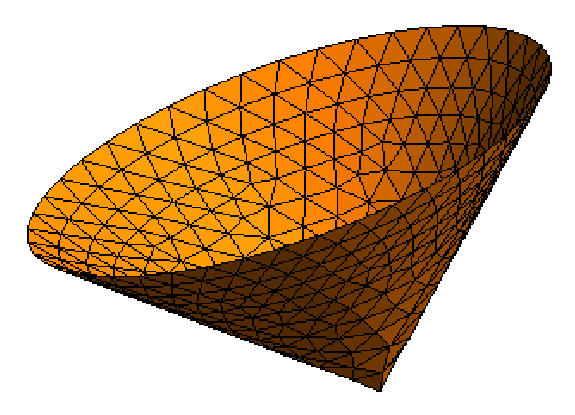
\includegraphics[width=70mm]{cone.eps}}


\paragraph{\numb section 3.\numb parag 21.
\special{ps: gsave 0.6 setgray}Singularities, again\special{ps: grestore}}

{\bf The code described in this section does not work yet.
It should be regarded as a mere declaration of intentions.}
\medskip

Besides vertices like the one described in paragraph \numb section 3.\numb parag 20, another
kind of singularity appears when we intersect two manifolds which have a tangency point.
This happens if we choose {\codett cr = 0.5} in paragraph \numb section 3.\numb parag 18 or
\numb section 3.\numb parag 19.

We focus on the piece of cylinder from paragraph \numb section 3.\numb parag 19
(which is to be subsequently {\codett join}ed with a sphere with two holes).

\verbatim
   Manifold cylinder = RR3.implicit ( y*y + (z-0.5)*(z-0.5) == 0.25 );
   Manifold infinity = cylinder.implicit ( x*x + y*y + z*z == 1. );
   Cell V ( tag::vertex );  x(V) = 0.;  y(V) = 0.;  z(V) = 1.;
   Mesh circle_1 ( tag::progressive,
                   tag:: start_at, V, tag::towards, { 1., 1., 0. },
                   tag::singular, V, tag::desired_length, 0.1       );
   Mesh circle_2 ( tag::progressive,
                   tag:: start_at, V, tag::towards, { -1., -1., 0. },
                   tag::singular, V, tag::desired_length, 0.1         );

   cylinder.set_as_working_manifold();
   Cell W = circle_1.cell_in_front_of(V).tip();
   Mesh piece_of_cyl ( tag::progressive, tag::boundary, circle_1, circle_2,
                       tag::start_at, W, tag::towards, { -1., 1., 0. },
                       tag::singular, V, tag::desired_length, 0.1           );
\endverbatim

\bigskip
\centerline{\includegraphics[width=85mm]{cyl.eps}}
\bigskip

{\ManiFEM} accepts as {\codett Manifold} a self-intersecting set like {\codett infinity}.
However, in the {\codett Mesh} constructor we must specify {\codett V} as singular point.

Unlike in paragraph \numb section 3.\numb parag 19, here we cannot {\codett join} the two
meshes {\codett circle\_1} and {\codett circle\_2}.
{\ManiFEM} is unable to join two closed polygonal lines having a vertex in common;
in other words, it does not handle self-intersecting {\codett Meshes}.
This is why we provide the two pieces of boundary separately.
\vfil\eject


\paragraph{\numb section 3.\numb parag 22. Non-uniform meshing}

The {\codett desired\_length} may be a non-constant function.

\verbatim
   Function d = 0.03 + 0.04 * ( (x+0.3)*(x+0.3) + (y-0.9)*(y-0.9) );
   Manifold circle = RR2.implicit ( x*x + y*y == 1. );
   Mesh outer ( tag::progressive, tag::desired_length, d );
   Manifold ellipse = RR2.implicit ( x*x + (y-0.37)*(y-0.37) + 0.3*x*y == 0.25 );
   Mesh inner ( tag::progressive, tag::desired_length, d );
   Mesh bdry ( tag::join, outer, inner.reverse() );
   RR2.set_as_working_manifold();
   Mesh disk ( tag::progressive, tag::boundary, bdry, tag::desired_length, d );
\endverbatim

\centerline{\includegraphics[width=90mm]{disk-non-unif.eps}}
\medskip

Compare with the mesh in paragraph \numb section 3.\numb parag 3.

It is the user's responsibility to provide a {\codett desired\_length} which takes positive
values at all points of the future mesh.
Also, {\codett desired\_length} should be a reasonably smooth function;
sharp variations should be avoided.


\paragraph{\numb section 3.\numb parag 23. 
\special{ps: gsave 0.6 setgray}Changing the Riemann metric\special{ps: grestore}}

{\bf The code described in this section does not work yet.
It should be regarded as a mere declaration of intentions.}
\medskip

We can attach a non-uniform metric to our manifold; as a consequence, for a constant
{\codett desired\_length}, the apparent segment length will vary from zone to zone.
For instance, in the code below we set a metric which increases the measured length
of the segments close to the narrow part of the domain.
As a consequence, the meshing algorithm, while trying to build a mesh of constant
{\codett desired\_length}, will choose shorter segments in the proximity of the narrow zone
(because the length measured by the Riemann metric will be larger than the length
we see in the drawing), thus producing the same result as in paragraph
\numb section 3.\numb parag 22.

\verbatim
   Manifold RR2 ( tag::Euclid, tag::of_dim, 2 );
   Function xy = RR2.build_coordinate_system ( tag::Lagrange, tag::of_degree, 1 );
   Function x = xy[0],  y = xy[1];
   Function d = 0.3 + 0.5 * ( (x+0.3)*(x+0.3) + (y-0.9)*(y-0.9) );
   RR2.set_metric ( 1. / d );
   
   Manifold circle = RR2.implicit ( x*x + y*y == 1. );
   Mesh outer ( tag::progressive, tag::desired_length, 0.1 );
   Manifold ellipse = RR2.implicit ( x*x + (y-0.37)*(y-0.37) + 0.3*x*y == 0.25 );
   Mesh inner ( tag::progressive, tag::desired_length, 0.1 );
   Mesh bdry ( tag::join, outer, inner.reverse() );
   RR2.set_as_working_manifold();
   Mesh disk ( tag::progressive, tag::boundary, bdry, tag::desired_length, 0.1 );
\endverbatim

These two approaches (the one described in paragraph \numb section 3.\numb parag 22 and the
one described here) can be used interchangeably.
It is possible to use both in the same code, but the code will become rather obscure.


\paragraph{\numb section 3.\numb parag 24. 
\special{ps: gsave 0.6 setgray}Anisotropic metric\special{ps: grestore}}

{\bf The code described in this section does not work yet.
It should be regarded as a mere declaration of intentions.}
\medskip

The technique described in paragraph \numb section 3.\numb parag 23 can be generalized to
an anisotropic Riemann metric.
We define the metric by means of a square matrix $M$.
$M$ must be symmetric positive definite.
The arguments of {\codett set\_metric} are $ m_{11} $, $ m_{12} $ and $ m_{22} $ for two dimensions,
$ m_{11} $, $ m_{12} $, $ m_{13} $, $ m_{22} $, $ m_{23} $ and $ m_{33} $ for three dimensions.

\medskip
\centerline{\includegraphics[width=90mm]{disk-anisotrop.eps}}
\medskip

\verbatim
   Manifold RR2 ( tag::Euclid, tag::of_dim, 2 );
   Function xy = RR2.build_coordinate_system ( tag::Lagrange, tag::of_degree, 1 );
   Function x = xy[0],  y = xy[1];
   Function d = 0.3 + (x+0.3)*(x+0.3) + (y-0.9)*(y-0.9);
   RR2.set_metric ( 1. + 1./d, -3./d, 1. + 9./d );
   // or, equivalently :
   // RR2.set_metric ( tag::principal_part, 1.,
   //                  tag::deviatoric_part, 1./d, -3./d, 9./d );

   Manifold circle = RR2.implicit ( x*x + y*y == 1. );
   Mesh outer ( tag::progressive, tag::desired_length, 0.1 );
   Manifold ellipse = RR2.implicit ( x*x + (y-0.37)*(y-0.37) + 0.3*x*y == 0.25 );
   Mesh inner ( tag::progressive, tag::desired_length, 0.1 );
   Mesh bdry ( tag::join, outer, inner.reverse() );
   RR2.set_as_working_manifold();
   Mesh disk ( tag::progressive, tag::boundary, bdry, tag::desired_length, 0.1 );
\endverbatim

Compare with the mesh in paragraph \numb section 3.\numb parag 3.

This result cannot be achieved using the approach of paragraph \numb section 3.\numb parag 22
(by setting a non-constant {\codett desired\_length}).


%%%%%%%%%%%%%%%%%%%%%%%%%%%%%%%%%%%%%%%%%%%%%%%%%%%%%%%%%%%%%%%%%%%%%%%%%%%%%%%%%%%%%%%%%%%%%%%
%%%%%%%%%%%%%%%%%%%%%%%%%%%%%%%%%%%%%%%%%%%%%%%%%%%%%%%%%%%%%%%%%%%%%%%%%%%%%%%%%%%%%%%%%%%%%%%



\section{\numb section 5. \special{ps: gsave 0.6 setgray}Quotient manifolds\special{ps: grestore}}

{\bf The code described in this section does not work yet.
It should be regarded as a mere declaration of intentions.}
\medskip

The roots of {\maniFEM} go back to a PhD thesis in 2002
% (or even earlier, to a Master thesis in 1997)
where finite elements on a torus were implemented in {\tt FORTRAN}.%
\footnote *{\parbox{\ftntfont\baselineskip=3pt
See % C.~Barbarosie, Optimization of perforated domains through homogenization,
% Structural Optimization 14, 1997
C.~Barbarosie, Shape optimization of periodic structures,
Computers \& Structures 30, 2003}}
The torus is meant as a mere quotient manifold between $ \RR^2 $ and a group of
translations of $ \RR^2 $ with two generators; you may think of it as $ \RR^2/\ZZ^2 $.
It should be stressed that this manifold is not the usual ``donut'' built in paragraph
\numb section 2.\numb parag 14.
The quotient torus is a Riemann manifold with no curvature; it is locally Euclidian
(that is, locally isometric to open sets of $ \RR^2 $); we may call it ``flat torus''.
It cannot be embedded in $ \RR^3 $, much less be represented graphically.
An unfolded mesh in $ \RR^2 $ can be represented graphically, where vertices and segments
from the torus are drawn more than once.

One of the goals of {\maniFEM} is to deal with meshes on quotient manifolds.
Different quotient operations can be used, with groups of translations of $ \RR^2 $ but also
with other groups of transformations.


\paragraph{\numb section 5.\numb parag 1. \special{ps: gsave 0.6 setgray}A one-dimensional circle\special{ps: grestore}}

{\bf The code described in this paragraph does not work yet.
It should be regarded as a mere declaration of intentions.}

Here is the closed curve $ \RR/\ZZ $.
We define it as a segment from {\codett A} to {\codett A}, with a specified {\codett jump}.

\verbatim
   // begin with the one-dimensional line
   Manifold RR ( tag::Euclid, tag::of_dim, 1 );
   Function x = RR.build_coordinate_system ( tag::Lagrange, tag::of_degree, 1 );

   // define an action on RR2 (a translation)
   Manifold::Action g;  g(x) = x+1;
   Manifold circle = RR.quotient ( g );

   // one vertex is enough to start the process
   Cell A ( tag::vertex );  x(A) = 0.02;
   // with this vertex, we build a segment
   Mesh seg ( tag::segment, A.reverse(), A, tag::divided_in, 10, tag::jump, g );
\endverbatim

We do not bother with the graphical representation of this one-dimensional mesh.


\paragraph{\numb section 5.\numb parag 2. \special{ps: gsave 0.6 setgray}A flat torus\special{ps: grestore}}

{\bf The code described in this paragraph does not work yet.
It should be regarded as a mere declaration of intentions.}

Here is the classical example of $ \RR^2/\ZZ^2 $.

\verbatim
   // begin with the usual two-dimensional space
   Manifold RR2 ( tag::Euclid, tag::of_dim, 2 );
   Function xy = RR2.build_coordinate_system ( tag::Lagrange, tag::of_degree, 1 );
   Function x = xy[0], y = xy[1];

   // define two actions on RR2 (translations)
   Manifold::Action g1, g2;
   g1(x,y) = (x+1) && y;
   g2(x,y) = x && (y+1);
   Manifold torus_manif = RR2.quotient ( g1, g2 );

   // one vertex is enough to start the process
   Cell A ( tag::vertex );  x(A) = 0.02;  y(A) = 0.02;
   // with this vertex, we build two segments
   Mesh seg_horiz ( tag::segment, A.reverse(), A,
                    tag::divided_in, 10, tag::jump, g1 );
   Mesh seg_vert  ( tag::segment, A.reverse(), A,
                    tag::divided_in, 10, tag::jump, g2 );
   // and a rectangle
   Mesh torus ( tag::rectangle, seg_horiz, seg_vert,
                seg_horiz.reverse(), seg_vert.reverse() );

   // it would be meaningless to export 'square' as a msh file
   // we can however export an unfolded mesh :
   torus.unfold(-0.5,-0.2,0.5,0.2).export_msh ("unfolded-torus.msh");
\endverbatim

We have added a shadow representing the periodicity cell $ [0,1]^2 $.
This gives a hint about the segments being repeated by the unfolding.


\paragraph{\numb section 5.\numb parag 3. \special{ps: gsave 0.6 setgray}A skew flat torus\special{ps: grestore}}

{\bf The code described in this paragraph does not work yet.
It should be regarded as a mere declaration of intentions.}

We can build a skew torus by simply choosing other actions on {\codett RR2}.

\verbatim
   Manifold::Action g1, g2;
   g1(x,y) = (x+1)   && (y+0.1);
   g2(x,y) = (x+0.1) && (y+1);
   Manifold torus_manif = RR2.quotient ( g1, g2 );
\endverbatim

Again, we have added a shadow representing the periodicity cell, this time a parallelogram.


\paragraph{\numb section 5.\numb parag 4. \special{ps: gsave 0.6 setgray}A curved circle\special{ps: grestore}}

{\bf The code described in this paragraph does not work yet.
It should be regarded as a mere declaration of intentions.}

We are now in a position to resume the example in paragraph \numb section 2.\numb parag 13,
this time in a less cumbersome manner.

\verbatim
   Manifold RR ( tag::Euclid, tag::of_dim, 1 );
   Function theta = RR.build_coordinate_system ( tag::Lagrange, tag::of_degree, 1 );
   const double pi = 3.1415926536;
   Manifold::Action g;  g(theta) = theta + 2*pi;
   Manifold circle = RR.quotient ( g );

   Cell A ( tag::vertex );  theta(A) = 0.;
   Mesh seg ( tag::segment, A.reverse(), A, tag::divided_in, 10, tag::jump, g );

   // define new coordinates x and y as arithmetic expressions of theta
   Function x = cos(theta), y = sin(theta);
   // forget about theta; in future statements, x and y will be used
   circle.set_coordinates ( x && y );
   seg.export_msh ("circle.msh");
\endverbatim


\paragraph{\numb section 5.\numb parag 5. \special{ps: gsave 0.6 setgray}A cylinder\special{ps: grestore}}

{\bf The code described in this paragraph does not work yet.
It should be regarded as a mere declaration of intentions.}

Here is how to build a cylinder in $ \RR^3 $ :

\verbatim
   Manifold RR2 ( tag::Euclid, tag::of_dim, 2 );
   Function theta_z =
      RR2.build_coordinate_system ( tag::Lagrange, tag::of_degree, 1 );
   Function theta = theta_z[0], z = theta_z[1];
   const double pi = 3.1415926536;
   Manifold::Action g;  g( theta, z ) = (theta+2*pi) && z;
   Manifold cylinder_manif = RR2.quotient ( g );

   Cell A ( tag::vertex );  theta(A) = 0.; z(A) = -1.;
   Cell B ( tag::vertex );  theta(B) = 0.; z(B) =  1.;
   Mesh AA ( tag::segment, A.reverse(), A, tag::divided_in, 10, tag::jump,  g );
   Mesh AB ( tag::segment, A.reverse(), B, tag::divided_in, 10 );  // no jump
   Mesh BB ( tag::segment, B.reverse(), B, tag::divided_in, 10, tag::jump, -g );
   Mesh cylinder ( tag::rectangle, AA, AB, BB, AB.reverse() );

   // define new coordinates x and y as arithmetic expressions of theta
   Function x = cos(theta), y = sin(theta);
   // forget about theta; in future statements, x, y and z will be used
   cylinder_manif.set_coordinates ( x && y & z );
   cylinder.export_msh ("circle.msh");
\endverbatim


\paragraph{\numb section 5.\numb parag 6. \special{ps: gsave 0.6 setgray}A curved torus\special{ps: grestore}}

{\bf The code described in this paragraph does not work yet.
It should be regarded as a mere declaration of intentions.}

We are now in a position to resume the example in paragraph \numb section 2.\numb parag 14,
this time by using the quotient manifold $ \RR^2/\ZZ^2 $ introduced in paragraph
\numb section 5.\numb parag 2.

\verbatim
   Manifold RR2 ( tag::Euclid, tag::of_dim, 2 );
   Function ab = RR2.build_coordinate_system ( tag::Lagrange, tag::of_degree, 1 );
   Function alpha = ab[0], beta = ab[1];
   const double pi = 3.1415926536;
   Manifold::Action g1, g2;
   g1(alpha,beta) = (alpha+2.*pi) && beta;
   g2(alpha,beta) = alpha && (beta+2.*pi);
   Manifold torus_manif = RR2.quotient ( g1, g2 );

   Cell A ( tag::vertex );  alpha(A) = 0.;  beta(A) = 0.;
   Mesh seg_horiz ( tag::segment, A.reverse(), A,
                    tag::divided_in, 10, tag::jump, g1 );
   Mesh seg_vert  ( tag::segment, A.reverse(), A,
                    tag::divided_in, 10, tag::jump, g2 );
   Mesh torus ( tag::rectangle, seg_horiz, seg_vert,
                seg_horiz.reverse(), seg_vert.reverse() );

   // parametrize the donut
   const double big_radius = 3., small_radius = 1.;
   // define x, y and z as functions of alpha and beta
   Function x = ( big_radius + small_radius*cos(beta) ) * cos(alpha),
            y = ( big_radius + small_radius*cos(beta) ) * sin(alpha),
            z = small_radius*sin(beta);

   // forget about alpha and beta :
   torus.set_coordinates ( x && y && z );
   // in future statements (e.g. for graphical representation)
   // x, y and z will be used, not alpha nor beta :
   torus.export_msh ("torus.msh");

\endverbatim


%%%%%%%%%%%%%%%%%%%%%%%%%%%%%%%%%%%%%%%%%%%%%%%%%%%%%%%%%%%%%%%%%%%%%%%%%%%%%%%%%%%%%%%%%%%%%%%
%%%%%%%%%%%%%%%%%%%%%%%%%%%%%%%%%%%%%%%%%%%%%%%%%%%%%%%%%%%%%%%%%%%%%%%%%%%%%%%%%%%%%%%%%%%%%%%



\section{\numb section 6. \special{ps: gsave 0.6 setgray}Fields, functions and variational formulations\special{ps: grestore}}

{\bf The code described in this section is outdated and does not work.}

\paragraph{\numb section 6.\numb parag 1. \special{ps: gsave 0.6 setgray}Fields and functions\special{ps: grestore}}

Consider the mesh built by the code below.

\verbatim
   Mesh::intended_dimension = 2; // topological dimension
   Mesh::initialize();
   auto & xy = NumericField::multi_dim ("size", 2, "lives on", "points");	
   auto & x = xy[0], & y = xy[1];
   auto & u = NumericField::one_dim ("lives on", "points");
   auto SW = Cell::point ("SW"); x(SW) = -1.1; y(SW) = 0.3;
   auto SE = Cell::point ("SE"); x(SE) = 1; y(SE) = 0;
   auto NE = Cell::point ("NE"); x(NE) = 1; y(NE) = 1;
   auto NW = Cell::point ("NW"); x(NW) = -1; y(NW) = 1;
   auto south ( tag::segment, SW.reverse(), SE, tag::divided_in, 4, xy );
   auto east  ( tag::segment, SE.reverse(), NE, tag::divided_in, 2, xy );
   auto north ( tag::segment, NE.reverse(), NW, tag::divided_in, 4, xy );
   auto west  ( tag::segment, NW.reverse(), SW, tag::divided_in, 2, xy );
   auto rect_mesh ( tag::rectangle, south, east, north, west, xy );
\endverbatim

Note that, besides the {\codett NumericField} objects {\codett x} and {\codett y}
which we have already encountered in paragraph \numb section 1.\numb parag 1,
we introduce another {\codett NumericField}, {\codett u}, which is meant to hold
the values of the solution of some PDE.

We now declare two functions defined on the mesh, linked to the two fields {\codett x} and
{\codett y}.
We can declare each function individually, as we did in paragraph \numb section 1.\numb parag 1,
or we can declare the pair and then extract each component :

\verbatim
   auto & xxyy = FunctionOnMesh::from_field ( xy, "Lagrange degree one" );
   auto & xx = xxyy[0], & yy = xxyy[1];
\endverbatim

These functions are described as {\codett "Lagrange degree one"}, which means that they vary
linearly along segments and also inside triangles.
On quadrilaterals, they are polynomials of degree one, meaning they have a linear part plus
a bi-linear one.

We can also declare an unknown function and a test function, to be used in a future variational
problem :

\verbatim
   auto & uu = FunctionOnMesh::unknown ( u, "Lagrange degree one");
   auto & w = FunctionOnMesh::test ( uu );
\endverbatim

The unknown {\codett uu} is related to the {\codett NumericField} previously declared,
{\codett u}, which provides space to hold, at each vertex of the mesh, a real value.
Hopefully, at the end of the day these will be the values of the solution of our PDE.
The test function does not need to hold any values.
The test function is an abstract object whose only use is to express the
variational formulation.

{\codett FunctionOnMesh} objects obey to usual arithmetic rules.
For instance, {\codett (xx+yy*w)/uu} is a valid expression in \maniFEM.
They can also be differentiated, like in {\codett (xx*yy).deriv(xx)}.
Note that this expression will be evaluated right away, producing the result
{\codett yy}, while expressions involving an unknown function or a test function
will produce a delayed derivative object, to be evaluated later.
Thus, {\codett w.deriv(xx)} will be evaluated only after replacing the test function
{\codett w} by some function in a base of a discretized Hilbert space.

{\codett FunctionOnMesh} objects can also be integrated through their method
{\codett integrate}, which produces a delayed integral expression.
The integral is not evaluated right away, but only later, with the use of an
{\codett Integrator} object (which could be a Gauss quadrature).

Integral expressions are stored as objects belonging to the class\hfil\break
{\codett FunctionOnMesh::combinIntegrals}.
These objects can be equated by using their\hfil\break
{\codett operator==}, which returns a {VariationalProblem} object.
Thus, the operator\hfil\break
{\codett FunctionOnMesh::combinIntegrals::operator==} acts as a factory function
for\hfil\break {\codett VariationalProblem} objects.
For instance, {\codett x.integrate(rect\_mesh) == y.integrate(south)} is a syntactically valid
expression which would produce a {\codett VariationalProblem} but actually
gives a run-time error because the {\codett operator==} checks that the right hand side
of the variational problem actually contains a function declared as uknown and one
declared as test, and that the left hand side contains a test function but no unknown.
Here is a more meaningful example :

\verbatim
   auto & var_pb =
       ( uu.deriv(xx)*w.deriv(xx) + uu.deriv(yy)*w.deriv(yy) ) .integrate(rect_mesh)
       == w.integrate(rect_mesh) + w.integrate(south);
\endverbatim

Note how we can mix integrals on different domains; recall that {\codett south} is
a side of {\codett rect\_mesh}.

Dirichlet-type boundary conditions are implemented through the directive
{\codett prescribe\_on} followed by one or more equalities.

\verbatim
   var_pb.prescribe_on (north);  uu == 0.;          w == 0.;
   var_pb.prescribe_on (east);   uu == xx*(1.-yy);  w == 0.;
   var_pb.prescribe_on (west);   uu == 0.;          w == 0.;
\endverbatim


%%%%%%%%%%%%%%%%%%%%%%%%%%%%%%%%%%%%%%%%%%%%%%%%%%%%%%%%%%%%%%%%%%%%%%%%%%%%%%%%%%%%%%%%%%%%%%%
%%%%%%%%%%%%%%%%%%%%%%%%%%%%%%%%%%%%%%%%%%%%%%%%%%%%%%%%%%%%%%%%%%%%%%%%%%%%%%%%%%%%%%%%%%%%%%%



\section{\numb section 7. \special{ps: gsave 0.6 setgray}Finite elements and integrators\special{ps: grestore}}

{\bf The code described in this section is outdated and does not work.}

Let's take over the example in paragraphs \numb section 1.\numb parag 9 and
\numb section 6.\numb parag 1.

The last few lines of code look rather simple :

\verbatim
   auto & fe = FiniteElement::Lagrange ("Q1");
   fe.set_integrator ("on cells of dimension", 1, "gauss", 3, "nodes");
   fe.set_integrator ("on cells of dimension", 2, "gauss", 9, "nodes");
   fe.discretize ( var_pb );
\endverbatim

This simplicity hides from the final user a complicated process : the discretization
of the variational formulation by a finite element.


\paragraph{\numb section 7.\numb parag 2. \special{ps: gsave 0.6 setgray}Finite elements\special{ps: grestore}}

The notion of a finite element is quite complex.
The purpose of a {\codett FiniteElement} is to build a list of functions, say, $ \psi $,
defined on our mesh.
The linear span of these functions will be a discretized Hilbert space.
The {\codett FiniteElement} should replace, in the variational formulation,
the unknown function by one $ \psi $, the test function by another $ \psi $ and,
by evaluating the integrals, obtain the coefficients of a system of linear equations.
Some external solver will then solve the system, and it is the job of the finite element
to transform back the vector produced by the solver into a function defined on our mesh.

Computing each integral is a somewhat separate process; it's the job of an {\codett Integrator}
which could be a Gauss quadrature or some other procedure like symbolic integration.
When a Gauss quadrature is used, the separation between a {\codett FiniteElement}'s job
and the {\codett Itegrator}'s job is not very sharp because often the Gauss quadrature is
perfomed not on the physical cell but rather on a master element which is built and
handled by the {\codett FiniteElement}.
The authors of {\maniFEM} have tried to separate these two concepts
as much as possible, especially because some users may want to use a {\codett FiniteElement}
with no master element, or an {\codett Integrator} acting directly on the physical cell.

Thus, there is a base class {\codett FiniteElement} and a derived class
{\codett FiniteElement::withMaster} which keeps, as an extra attribute, the map transforming
the master element to the current physical cell.
This map depends of course on the geometry of the cell and thus it must be computed from
scratch each time we begin integrating on a new cell.
We say that the {\codett FiniteElement} is docked on a new {\codett Cell};
the method {\codett dock\_on} performs this operation.
This method is element-specific, each type of finite element having its own class.

For instance, the class {\codett FiniteElement::Lagrange\_Q1} is a class derived from
\hfil\break{\codett FiniteElement::withMaster}.
It will only {\codett dock\_on} quadrilaterals (two-dimensional {\codett Cell}s
with four sides).
Recall that in {\maniFEM} the vertices do not have necessarily any number attached.
When we create a {\codett FiniteElement::Lagrange\_Q1} object, it will enumerate vertices
of the mesh if a mesh exists already, and it will prepare the ground for vertices created
in the future to be enumerated, too.
This enumeration is useful to identify a vector of real numbers with the values
(at each vertex) of a function defined on the mesh.
When docking on a cell, the {\codett FiniteElement::Lagrange\_Q1} object will build four
``shape functions'', a transformation map (from a master element occuppying the square
$ [-1, 1]^2 $ to the current cell) and the jacobian of this transformation.


%%%%%%%%%%%%%%%%%%%%%%%%%%%%%%%%%%%%%%%%%%%%%%%%%%%%%%%%%%%%%%%%%%%%%%%%%%%%%%%%%%%%%%%%%%%%%%%
%%%%%%%%%%%%%%%%%%%%%%%%%%%%%%%%%%%%%%%%%%%%%%%%%%%%%%%%%%%%%%%%%%%%%%%%%%%%%%%%%%%%%%%%%%%%%%%



\section{\numb section 8. A closer look at cells and meshes}

This section gives details about cells and meshes.


\paragraph{\numb section 8.\numb parag 1. Building cells and meshes}

As we have already seen in examples in previous sections, cells and meshes are created
by declaring them as {\codett Cell} or {\codett Mesh} objects and by providing specific
options to their constructor, by means of {\codett tag}s. For instance :

\verbatim
   Cell SW ( tag::vertex ); // and the same for vertices SE, NE, NW
   Mesh south ( tag::segment, SW.reverse(), SE, tag::divided_in, 10 );
   // similar declarations of east, north, west
   Mesh rectangle ( tag::rectangle, south, east, north, west );
\endverbatim

Paragraph \numb section 9.\numb parag 2 gives more details about {\codett tag}s.

Internally, {\maniFEM} implements cells and meshes as persistent obejcts, built
using the {\codett new} operator and thus having no syntactic scope.
Objects belonging to classes {\codett Cell} and {\codett Mesh} are just a wrapper
around a persistent core (cell or mesh).
When they go out of scope, the wrappers are destroyed but the core remains alive.
If a cell or mesh is no longer needed, the user must explicitly dispose of it,
as explained in paragraph \numb section 9.\numb parag 3.

Cells and meshes are unique objects, it makes no sense to copy them.
A statement like {\codett Cell copy\_of\_A = A} will make a copy of the wrapper
but it will refer to the same cell {\codett A}.
If you change e.g.\ a coordinate of {\codett copy\_of\_A}, the coordinate of {\codett A}
will also change.
That is, wrapper classes {\codett Cell} and {\codett Mesh} can be viewed as
customized pointers.
This is useful if we need to create many meshes in a loop, as shown in paragraph
\numb section 8.\numb parag 2.
However, there are operations which do create a new cell or mesh.
There are also operations which create a new cell or mesh only if necessary,
otherwise they will return an existing cell or mesh.
Paragraph \numb section 8.\numb parag 10 gives a complete list.

Recall that, in \maniFEM, cells and meshes are oriented.
When a cell is declared, it is built as positive and has no reverse.
Its reverse is a negative cell and will be built only if necessary.
Cells have a method {\codett reverse} which does the following.
It checks if the reverse object has already been built; if yes, it returns that object;
otherwise, it builds the reverse cell on-the-fly and returns it.
Paragraph \numb section 8.\numb parag 7 gives a more detailed explanation about
orientation of cells and meshes.
% See also paragraph \numb section 9.\numb parag 6.

{\codett Mesh}es have also a {\codett reverse} method.
Note that reverse meshes exist always (negative meshes are temporary objects built
on-the-fly).

At a basic level, the only situation when you need the {\codett reverse} method  for cells is
when you declare a segment {\codett Mesh} (you must provide a negative {\codett Cell} as
starting point).
You will occasionaly need to use the {\codett reverse} method for meshes (for instance, if you
intend to {\codett join} two meshes, their common boundary must have a certain orientation when
seen from a mesh and the opposite orientation when seen from the other mesh).
In the example in paragraph \numb section 1.\numb parag 3,
reverses of meshes {\codett CD} and {\codett BC} are used.


\paragraph{\numb section 8.\numb parag 2. A ring-shaped mesh}

For creating many meshes within a cycle, we can view a {\codett Cell} object as a
(customized) pointer to a persistent core cell, and the same for {\codett Mesh}es.
They are cheap to store and to copy.
We call these customized pointers ``wrappers''; their behaviour is described in some detail in
paragraph \numb section 9.\numb parag 3.

\verbatim
   Manifold RR2 ( tag::Euclid, tag::of_dim, 2 );
   Function xy = RR2.build_coordinate_system ( tag::Lagrange, tag::of_degree, 1 );
   Function x = xy[0],  y = xy[1];

   short int n_sectors = 15;
   double step_theta = 8*atan(1.)/n_sectors;
   short int radial_divisions = 10;
   short int rot_divisions = 5;
\endverbatim
   
\centerline{\includegraphics[width=10cm]{ring.eps}}

\verbatim
   // start the process by building a segment
   Cell ini_A ( tag::vertex );  x(ini_A) = 1.;  y(ini_A) = 0.;
   Cell ini_B ( tag::vertex );  x(ini_B) = 2.;  y(ini_B) = 0.;
   Mesh ini_seg ( tag::segment, ini_A.reverse(), ini_B,
                  tag::divided_in, radial_divisions     );
   Mesh prev_seg = ini_seg;
   Cell A = ini_A,  B = ini_B;
   list < Mesh > sectors;

   for ( short int i = 1; i < n_sectors; i++ )
   {  double theta = i * step_theta;
      // we build two new points
      Cell C ( tag::vertex ); x(C) = cos(theta);    y(C) = sin(theta);
      Cell D ( tag::vertex ); x(D) = 2.*cos(theta); y(D) = 2.*sin(theta);
      // and three new segments
      Mesh BD ( tag::segment, B.reverse(), D, tag::divided_in, rot_divisions );
      Mesh DC ( tag::segment, D.reverse(), C, tag::divided_in, radial_divisions );
      Mesh CA ( tag::segment, C.reverse(), A, tag::divided_in, rot_divisions );
      Mesh quadr ( tag::quadrangle, prev_seg, BD, DC, CA );
      sectors.push_back ( quadr );
      prev_seg = DC.reverse();
      A = C;  B = D;                                                     }

   // we now build the last sector, thus closing the ring
   // prev_seg, A and B have rotated during the construction process
   // but ini_seg, ini_A and ini_B are the same, initial, ones
   Mesh outer ( tag::segment, B.reverse(), ini_B, tag::divided_in, rot_divisions );
   Mesh inner ( tag::segment, ini_A.reverse(), A, tag::divided_in, rot_divisions );
   Mesh quadr ( tag::quadrangle, outer, ini_seg.reverse(), inner, prev_seg );
   sectors.push_back ( quadr );
   
   Mesh ring ( tag::join, sectors );
   ring.export_msh ("ring.msh");
\endverbatim

Note how we use a version of the {\codett Mesh} constructor with {\codett tag::join} taking as
argument a list of {\codett Mesh}es; we have already seen it in paragraph \numb section 2.\numb
parag 6.

We might have set curved boundaries by using a submanifold of $ \RR^2 $, like in paragraph
\numb section 2.\numb parag 8.

See also paragraph \numb section 9.\numb parag 7.


\paragraph{\numb section 8.\numb parag 3. Lists of cells inside a mesh}

As explained in paragraph \numb section 1.\numb parag 2, a {\codett Mesh} is
roughly a list of cells.
Internally, {\maniFEM} keeps lists of cells of each dimension, up the the maximum
dimension which is the dimension of the mesh.
Thus, if {\codett msh} is a {\codett Mesh} object, modelling a
mesh of triangles, then {\codett msh.core->cells[0]} is a list of pointers to cells holding
all vertices of that mesh, {\codett msh.core->cells[1]} is a list of pointers to cells
holding all segments and {\codett msh.core-> cells[2]} is a list of pointers to cells
holding all triangles.

Thus, we could use a loop like the one below for iterating over all segments of the mesh.

\verbatim
   for ( auto it = msh.core->cells[1].begin();
              it != msh.core->cells[1].end();  it++ )
   { auto seg = *it;  do_something_to (*seg);  }
\endverbatim

If you are not familiar with the notion of iterator over a list (or over other containers)
in {\tt C++}, this may be a good time for you to read an introductory book on the
{\tt C++} Standard Template Library (STL).

The {\codett auto} keyword tells the {\tt C++} compiler to guess the type of a variable
according to the expression used to initialize it.
Note that the above code only works for a positive mesh.
Paragraphs \numb section 8.\numb parag 5 and \numb section 8.\numb parag 6 describe
nicer ways to iterate over cells of a mesh.

On the other hand, a cell is roughly defined by its boundary which in turn is a mesh of
lower dimension.
Thus, if {\codett hex} is a {\codett Cell} object modelling a hexagon,
then {\codett hex.boundary()} is a {\codett Mesh} object modelling a
one-dimensional mesh (a closed chain of six segments).
So, if we want to iterate, say, over all vertices of that hexagon, we can use a 
loop like below.

\verbatim
   auto & li = hex.boundary().cells[0];
   for ( auto it = li.begin(); it != li.end(); it++ )
   { auto P = *it;  do_something_to (*P);  }
\endverbatim

Note that the above only works if {\codett hex} is a positive cell.
Also, we have no guarantee about the order in which the vertices will show up in the loop.
Paragraph \numb section 8.\numb parag 6 describes other ways of iterating over one-dimensional
meshes, which follow the natural order of the vertices or segments.


\paragraph{\numb section 8.\numb parag 5. Iterators over cells}

This paragraph assumes that the reader is familiar to the notion of iterator in {\tt C++}.
If this is not the case, you should read an introductory book on the {\tt C++}
Standard Template Library (STL) before proceeding.

As explained in paragraphs \numb section 1.\numb parag 2 and \numb section 8.\numb parag 3,
a mesh is essentially a collection of cells.
In many situations, we may want to iterate over all cells of a mesh.

Suppose we have a mesh {\codett msh} of rectangles.
If we want to do something to each rectangle, that is, to each two-dimensional cell,
we could use a code like

\verbatim
   for ( auto it = msh.core->cells[2].begin();
              it != msh.core->cells[2].end(); it++ )
   {  auto cll = *it;  do_something_to (*cll);  }
\endverbatim

This style is slightly cumbersome and doesn't work for negative meshes,
so we provide specific iterators.
The code above is equivalent to

\verbatim
   CellIterator it = msh.iter_over ( tag::cells_of_dim, 2 );
   for ( it.reset(); it.in_range(); it++ )
   {  Cell cll = *it;  do_something_to (cll);  }
\endverbatim

Paragraph \numb section 9.\numb parag 2 gives some details about tags.

In the above code you may note that these iterators obey to syntactic conventions
slightly different from the ones in the Standard Template Library.
We have chosen that, when we want to start an iteration process, we set the iterator in
a starting configuration by using a {\codett reset} method rather than through an assignment
like {\codett it = container.begin()}.
Similarly, when an iterator has offered access to all cells of a mesh and cannot find
other cells, it goes into a state which can be checked using its {\codett in\_range} method
rather than by testing equality with some abstract object like {\codett container.end()}.
We have kept the syntax {\codett it++} for advancing an iterator in the process of
running over cells, offering also the equivalent alteratives {\codett ++it} and
{\codett it.advance()}.
We have also kept the notation {\codett *it} for dereferencing a {\codett CellIterator};
this operation returns a reference to a {\codett Cell} object.
Of course, dereferencing a {\codett CellIterator} does not produce a new cell,
just provides access to a previously built cell (see also paragraph \numb section 8.\numb
parag 10).

If we want to iterate over all vertices of the mesh, we can use

\verbatim
   CellIterator it = msh.iter_over ( tag::cells_of_dim, 0 );
   for ( it.reset(); it.in_range(); it++ )
   {  Cell P = *it;  do_something_to (P);  }
   // or, equivalently :
   CellIterator it = msh.iter_over ( tag::vertices );
\endverbatim

If we want to iterate over all segments of the mesh, we can use

\verbatim
   CellIterator it = msh.iter_over ( tag::cells_of_dim, 1 );
   for ( it.reset(); it.in_range(); it++ )
   {  Cell seg = *it;  do_something_to (seg);  }
   // or, equivalently :
   CellIterator it = msh.iter_over ( tag::segments );
\endverbatim

Note that an iterator running through cells of maximum dimension, that is, of dimension equal
to the dimension of the mesh, may produce negative cells if the mesh contains them.
Paragraph \numb section 8.\numb parag 7 discusses this possibility.
Iterators over cells of lower dimension produce always positive cells.

We can force an iterator over cells of maximum dimension to produce only positive cells
by adding a {\codett tag::force\_positive} as in

\verbatim
   CellIterator it = msh.iter_over ( tag::cells_of_dim, 2, tag::force_positive );
\endverbatim

Note that it is not safe to modify a mesh while iterating over its cells.
After modifying a mesh, you may re-use a previously declared iterator by {\codett reset}ting it.
An exception to the above rule happens for one-dimensional meshes, described in paragraph
\numb section 8.\numb parag 6.

If we only want to know how many cells there are in a certain mesh,
instead of using {\codett msh.core->cells[d].size()} ({\codett d} being the desired
dimension of the cells) we may use the method {\codett number\_of} :

\verbatim
   short int d = 2;
   size_t n = msh.number_of ( tag::cells_of_dim, d );
\endverbatim

\noindent Expression {\codett msh.number\_of ( tag::vertices )} is equivalent to
{\codett msh.number\_of ( tag::cells\_ \_of\_dim, 0 )}, while {\codett msh.number\_of
( tag::segments ) } is equivalent to {\codett msh.number\_of ( tag:: ::cells\_of\_dim, 1 )}.

Paragraph \numb section 8.\numb parag 6 describes iterators specific to one-dimensional
meshes.


\paragraph{\numb section 8.\numb parag 6. Iterators over chains of segments}

One-dimensional meshes have a specific structure (technical details provided in
paragraph \numb section 9.\numb parag 14) so we provide specialized iterators.
Unlike the iterators described in paragraph \numb section 8.\numb parag 5,
which sweep the mesh in a rather unredictible order,
the iterators below follow the natural order of the cells (either vertices or segments)
given by the topology of the mesh.

The syntax is the same as for higher-dimensional meshes :

\verbatim
   Mesh chain ( tag::segment, A.reverse(), B, tag::divided_in, n );
   // A and B are (positive) vertices, n is an integer
   
   CellIterator it1 = chain.iter_over ( tag::cells_of_dim, 1 );
   for ( it1.reset(); it1.in_range(); it1++ )
   {  Cell seg = *it1;  do_something_to (seg);  }
   
   CellIterator it0 = chain.iter_over ( tag::cells_of_dim, 0 );
   for ( it0.reset(); it0.in_range(); it0++ )
   {  Cell P = *it0;  do_something_to (P);  }

   // or, equivalently,
   CellIterator it0 = chain.iter_over ( tag::vertices );
   CellIterator it1 = chain.iter_over ( tag::segments );
\endverbatim

Unlike iterators over cells of meshes of dimension 2 or higher, presented in paragraph
\numb section 8.\numb parag 5, iterators over one-dimensional meshes require the mesh
to be connected.

A connected one dimensional mesh can be either an open chain of segments or a closed one
(a loop).
For an open chain, {\codett it0} will begin at the first vertex and end at the last vertex,
{\codett it1} will begin at the first segment and end at the last segment.
For a loop, they will begin at some arbitrary vertex or segment in the chain and produce
all the vertices or segments following the natural order given by the topology of the mesh.

If we want to start at a specific location, we can make a {\codett reset} call with
one argument.
For iterators over vertices, this argument should be a vertex, while for iterators
over segments, this argument should be a segment.
If such an argument is given, then the iteration process will begin at that particular
vertex or segment.
This special kind of {\codett reset} can be used for an open chain or a closed one,
but beware : if applied to an open chain, the vertices or segments previous to the provided
argument will not show up in the iteration process.

Note that {\codett it0} produces positive points, while {\codett  it1} produces
oriented segments (positive or negative).
We may enforce that we only want positive segments by adding the {\codett tag::force\_positive},
as shown in paragraph \numb section 8.\numb parag 7.

There are also reversed versions of these iterators (they go backwards), obtained by adding
the {\codett tag::reverse} :

\verbatim
   CellIterator it1r = chain.iter_over ( tag::segments, tag::reverse );
   CellIterator it0r = chain.iter_over ( tag::vertices, tag::reverse );
\endverbatim

Method {\codett number\_of} works just as for higher-dimensional iterators (see paragraph
\numb section 8.\numb parag 5).

One-dimensional meshes have also methods {\codett first\_vertex}, {\codett last\_vertex},
{\codett first\_segment} and {\codett last\_segment} which return the cell described by their
names.
They should only be used for an open chain (not for a loop).
Note that both {\codett Mesh::first\_vertex} and {\codett Mesh::last\_vertex} return
positive vertices, unlike the {\codett Cell::base} method (described in paragraph
\numb section 1.\numb parag 2) which returns a negative vertex. [this should change]

Recall that it is not safe to modify a mesh while iterating over its cells.
After modifying a mesh, you may re-use a previously declared iterator by {\codett reset}ting it.
However, if you modify a one-dimensional mesh and change its topology
(cut a loop, thus making it an open chain, or contrarywise, close a chain,
thus making it a loop), then you cannot re-use
a previously declared iterator on that mesh (you must declare a new iterator).
A change in the code is planned; when we {\codett reset} an iterator, it will adapt itself
to the new shape of the mesh.

As explained in paragraph \numb section 8.\numb parag 10, dereferencing a {\codett CellIterator}
does not produce a new cell, just provides access to a previously built cell.


\paragraph{\numb section 8.\numb parag 7. Orientation of cells inside a mesh}

In \maniFEM, all cells and meshes are oriented.

This can be confusing sometimes, so let's have a closer look at a particular example.

{ \psfrag{A}{\special{ps: gsave 0 0 0.8 setrgbcolor}{\codett A}\special{ps: grestore}}
\psfrag{B}{\special{ps: gsave 0 0 0.8 setrgbcolor}{\codett B}\special{ps: grestore}}
\psfrag{C}{\special{ps: gsave 0 0 0.8 setrgbcolor}{\codett C}\special{ps: grestore}}
\psfrag{D}{\special{ps: gsave 0 0 0.8 setrgbcolor}{\codett D}\special{ps: grestore}}
\centerline{\includegraphics[width=4cm]{malha-tri.eps}} }

Consider a mesh {\codett tri\_mesh} made of triangles.
Unless requested otherwise, {\codett tri\_mesh} will be a positive mesh and all triangles
composing it will also be positive.
So, the triangles composing {\codett tri\_mesh} will have no reverse cell
(there is no need for such).

However, the segments must have reverse.
Consider triangle {\codett ABC} for instance.
Its boundary is made of three segments; let's look at {\codett AB} for example,
a segment having {\codett A} as base and {\codett B} as tip.
Now, a triangle {\codett BAD} (no offense intended) also exists as part of {\codett tri\_mesh}.
The boundary of {\codett BAD} is made of three segments, one of them being {\codett BA},
which has {\codett B} as base and {\codett A} as tip.
{\codett AB} and {\codett BA} are different {\codett Cell} objects;
each is the reverse of the other.
One of them is considered positive and the other is considered negative.
Which is which depends on which one was built first.
So, all inner segments must have a reverse;
segments on the boundary of {\codett tri\_mesh} will probably have no reverse.

For points (vertices), the situation is even more complex.
Segment {\codett AB} sees {\codett A} as negative because {\codett A} is its base,
but other segments like {\codett CA} see {\codett A} as positive.

Let's look again at iterators described in paragraph \numb section 8.\numb parag 5.
We now understand that there is no point to have an iterator over oriented
segments, or over oriented vertices, of {\codett tri\_mesh}.
That's why iterators over cells of lower dimension always produce positive cells.

We also understand that there is no difference between these two iterators :

\verbatim
   CellIterator it1 = tri_msh.iter_over ( tag::cells_of_dim, 2 );
   CellIterator it2 =
      tri_msh.iter_over ( tag::cells_of_dim, 2, tag::force_positive );
\endverbatim

\noindent because all triangles composing {\codett tri\_mesh} should be positive
(use {\codett it1}, it is slightly faster).
However, if some of the triangles are negative {\codett it1} will behave differently from
{\codett it2}.
For instance, if {\codett tri\_mesh} is the boundary of a polyhedron in $ \RR^3 $
and this polyhedron touches other polyhedra (there are shared faces), then it is
quite possible that some of the triangles in {\codett tri\_mesh} be negative.
If you are aware that your mesh may contain negative cells but
you want to iterate over their positive counterparts, use the {\codett tag::force\_positive}.

We now turn to iterators over one-dimensional meshes, described in paragraph
\numb section 8.\numb parag 6.
The two iterators below will probably have different behaviours,
depending on which segments happen to be positive :

\verbatim
   CellIterator it3 = ABC.boundary().iter_over ( tag::segments );
   CellIterator it4 =
      ABC.boundary().iter_over ( tag::segments, tag::force_positive );
\endverbatim

There is no difference between the two iterators below (both produce positive
points).

\verbatim
   CellIterator it5 = ABC.boundary().iter_over ( tag::vertices, tag::reverse );
   CellIterator it6 = ABC.boundary().reverse().iter_over( tag::vertices );
\endverbatim

However, the two iterators below are quite different.

\verbatim
   CellIterator it7 = ABC.boundary().iter_over ( tag::segments, tag::reverse );
   CellIterator it8 = ABC.boundary().reverse().iter_over ( tag::segments );
\endverbatim

Iterator {\codett it7} will produce segments {\codett AB}, {\codett CA}, {\codett BC}
(not necessarily beginning at {\codett AB}), while {\codett it8} will produce their reverses
{\codett BA}, {\codett AC}, {\codett CB} (not necessarily beginning at {\codett BA}).

Incidentally, note that a segment, say, {\codett BC}, may have no reverse,
for instance if it is on the boundary of {\codett tri\_mesh}.
However, its reverse {\codett CB} will be built on-the-fly (and will stay persistent)
as soon as you use the reverse mesh {\codett ABC.boundary().reverse()} in the declaration of
{\codett it6} (or {\codett it8}, whichever happens first in your code).


\paragraph{\numb section 8.\numb parag 8. Navigating inside a mesh}

Objects in class {\codett Mesh} have two methods, {\codett cell\_behind} and
{\codett cell\_in\_front\_of},
which provide access to the neighbours of a given cell within that mesh.
Together with methods {\codett base} and {\codett tip} of class {\codett Cell}
(mentioned in paragraph \numb section 1.\numb parag 2), they allow us to navigate inside
a mesh.

{ \psfrag{A}{\special{ps: gsave 0 0 0.8 setrgbcolor}{\codett A}\special{ps: grestore}}
\psfrag{B}{\special{ps: gsave 0 0 0.8 setrgbcolor}{\codett B}\special{ps: grestore}}
\psfrag{C}{\special{ps: gsave 0 0 0.8 setrgbcolor}{\codett C}\special{ps: grestore}}
\psfrag{D}{\special{ps: gsave 0 0 0.8 setrgbcolor}{\codett D}\special{ps: grestore}}
\psfrag{hex_1}{\special{ps: gsave 0 0 0.8 setrgbcolor}{\codett hex\_1}\special{ps: grestore}}
\psfrag{hex_2}{\special{ps: gsave 0 0 0.8 setrgbcolor}{\codett hex\_2}\special{ps: grestore}}
\centerline{\includegraphics[width=4cm]{malha-hex.eps}} }
\medskip

Consider the mesh {\codett hex\_msh} shown above, made of three hexagons.
Pick one of them, at random :

\verbatim
   CellIterator it1 = hex_msh.iter_over ( tag::cells_of_dim, 2 );
   it1.reset();
   Cell hex_1 = *it1;
\endverbatim

Now choose a random segment on the boundary of {\codett hex\_1} :

\verbatim
   CellIterator it2 = hex_1.boundary().iter_over ( tag::segments );
   it2.reset();
   Cell AB = *it2;
\endverbatim

Take its tip :

\verbatim
   Cell B = AB.tip();
\endverbatim

Suppose now we want the next segment, within the boundary of {\codett hex\_1} :

\verbatim
   Cell BC = hex_1.boundary().cell_in_front_of ( B );
\endverbatim

And now we may continue by taking the tip of {\codett BC} and then the segment
following it$\;$:

\verbatim
   Cell C = BC.tip();
   Cell CD = hex_1.boundary().cell_in_front_of ( C );
\endverbatim

\noindent an so forth (this is how iterators over vertices and segments of
one-dimensional meshes, described in paragraph \numb section 8.\numb parag 6,
are implemented internally).

Within the mesh {\codett hex\_msh}, we can navigate towards a neighbour hexagon :

\verbatim
   Cell hex_2 = hex_msh.cell_in_front_of ( CD );
\endverbatim

Since we have picked {\codett hex\_1} at random within {\codett hex\_msh},
as well as {\codett AB} within the boundary of {\codett hex\_1},
there is no guarantee that we actually are in the configuration shown in the
picture above.
That is, {\codett CD} may be on the boundary of {\codett hex\_msh};
there may be no neighbour hexagon {\codett hex\_2}.
If that is the case, the code above will produce an execution error.
See paragraph \numb section 8.\numb parag 9 for a way to check whether there is actually
a neighbour cell and thus avoid errors at execution time.

Note that faces point outwards.
For instance, {\codett CD} belongs to the boundary of {\codett hex\_1} and points
outwards, towards {\codett hex\_2}.
Thus, {\codett hex\_msh.cell\_in\_front\_of(CD)} produces {\codett hex\_2}.
On the other hand, {\codett hex\_msh.cell\_behind(CD)} is {\codett hex\_1}.

Note also that {\codett CD} does not belong to the boundary of {\codett hex\_2}.
If we take {\codett hex\_2.boundary() .cell\_in\_front\_of(D)} we will obtain not
{\codett CD} but its reverse, a distinct cell which we may call {\codett DC}.
We have that {\codett hex\_msh.cell\_in\_front\_of(DC)} is {\codett hex\_1} and
{\codett hex\_msh.cell\_behind(DC)} is {\codett hex\_2}.


\paragraph{\numb section 8.\numb parag 9. Navigating at the boundary of a mesh}

Consider the example in paragraph \numb section 8.\numb parag 8.
Suppose you try to get a neighbour hexagon which does not exist :

\verbatim
   Cell no_such_hex = hex_msh.cell_in_front_of ( AB );
\endverbatim

In {\codett DEBUG} mode, you will get an {\codett assertion error}.
In {\codett NDEBUG} mode, the behaviour is undefined
(often, a {\codett segmentation fault} will arise).
The {\codett DEBUG} mode is explained at the beginning of paragraph \numb section
9.\numb parag 12.

You may check the existence of the neighbour cell by using a
{\codett tag::may\_not\_exist} and then the cell's method {\codett exists} :

\verbatim
   Cell possible_hex = hex_msh.cell_in_front_of ( AB, tag::may_not_exist );
   if ( possible_hex.exists() ) do_something_to ( possible_hex );
   else cout << "no neighbour !" << endl;
\endverbatim

\noindent thus avoiding errors at execution time.

Paragraph \numb section 8.\numb parag 10 gives a complete list of operations which return
an existing cell or build a new one.


\paragraph{\numb section 8.\numb parag 10. Declaring cells and meshes}

As explained in paragraph \numb section 9.\numb parag 3, the {\codett Cell} class
is just a thin wrapper around a {\codett Cell::Core}, and similarly for {\codett Mesh}es.

Statements below build a new wrapper for an existing cell or mesh.
No new cell or mesh is created :

\verbatim
   Cell A = B;  // B is a Cell
   Cell C = *it;  // 'it' is a CellIterator
   Mesh msh_copy = msh;  // msh is a Mesh
   Mesh bd = cll.boundary();  // cll is a Cell of dimension at least 2
\endverbatim

Statements below search for an existing cell.
If the respective cell exists, (a new wrapper for) it is returned.
Otherwise, an {\codett assertion error} will occur in {\codett DEBUG} mode;
in {\codett NDEBUG} mode, the behaviour is undefined (often, a {\codett segmentation fault}
will arise).
The {\codett DEBUG} mode is explained at the beginning of paragraph \numb section
9.\numb parag 12.

\verbatim
   Cell A_rev = A.reverse ( tag::surely_exists );  //  A is a Cell
   // or, equivalently :
   Cell A_rev ( tag::reverse_of, A, tag::surely_exists );

   Cell tri1 = msh.cell_behind ( CD );  //  CD is a Cell, a face within msh
   Cell tri2 = msh.cell_in_front_of ( CD );
   // or, equivalently :
   Cell tri1 ( tag::behind_face, CD, tag::within_mesh, msh );
   Cell tri2 ( tag::in_front_of_face, CD, tag::within_mesh, msh );
   // or, equivalently :
   Cell tri1 = msh.cell_behind ( CD, tag::surely_exists );
   Cell tri2 = msh.cell_in_front_of ( CD, tag::surely_exists );
   // or, equivalently :
   Cell tri1 ( tag::behind_face, CD, tag::within_mesh, msh, tag::surely_exists );
   Cell tri2 ( tag::in_front_of_face, CD,
               tag::within_mesh, msh, tag::surely_exists );
\endverbatim

Note that reverse meshes exist always (negative meshes are temporary objects built
on-the-fly).

\verbatim
   Mesh rev_msh = msh.reverse();  // msh is a Mesh
\endverbatim

Statements below search for an existing cell.
If the respective cell exists, (a new wrapper for) it is returned.
Otherwise, a non-existent cell is returned
(an empty wrapper); the user has the possibility of inquiring the existence
of the returned cell using its method {\codett exists}, as illustrated in paragraph
\numb section 8.\numb parag 9.

\verbatim
   Cell A_rev = A.reverse ( tag::may_not_exist );  //  A is a Cell
   // or, equivalently :
   Cell A_rev ( tag::reverse_of, A, tag::may_not_exist );
   
   Cell tri1 = msh.cell_behind ( CD, tag::may_not_exist );
   //  CD is a Cell, a face within msh
   Cell tri2 = msh.cell_in_front_of ( CD, tag::may_not_exist );
   // or, equivalently :
   Cell tri1 ( tag::behind_face, CD, tag::within_mesh, msh, tag::may_not_exist );
   Cell tri2
      ( tag::in_front_of_face, CD, tag::within_mesh, msh, tag::may_not_exist );
\endverbatim

Statements below return a previously built cell, if it exists.
If that object does not exist, it is built on-the-fly.

\verbatim
   Cell A_rev = A.reverse();  // A is some Cell
   // or, equivalentely :
   Cell A_rev ( tag::reverse_of, A );
   // or, equivalentely :
   Cell A_rev = A.reverse ( tag::build_if_not_exists );
   // or, equivalentely :
   Cell A_rev ( tag::reverse_of, A, tag::build_if_not_exists );
\endverbatim

Statements below return a wrapper for a brand new cell or mesh :

\verbatim
   Cell A ( tag::vertex );
   Mesh AB ( tag::segment, A.reverse(), B, tag::divided_in, 15 );
   // B is another vertex Cell
   Mesh ABC ( tag::triangle, AB, BC, CA );
   //  BC and CA are segment Meshes, each having 15 segments Cells
   // ... and many other shapes ...
\endverbatim

Paragraph \numb section 9.\numb parag 6 explains similar operations on {\codett Cell::Core}s.


%%%%%%%%%%%%%%%%%%%%%%%%%%%%%%%%%%%%%%%%%%%%%%%%%%%%%%%%%%%%%%%%%%%%%%%%%%%%%%%%%%%%%%%%%%%%%%%
%%%%%%%%%%%%%%%%%%%%%%%%%%%%%%%%%%%%%%%%%%%%%%%%%%%%%%%%%%%%%%%%%%%%%%%%%%%%%%%%%%%%%%%%%%%%%%%



\section{\numb section 9. Technical details}

Sections \numb section 9 and \numb section 10 are meant for those intereseted in developing and
extending \maniFEM.
Of course the ultimate documentation is the source code; these sections can be used as
a guide through the source code.


\paragraph{\numb section 9.\numb parag 1. Namespaces and class names}

All names in {\maniFEM} are wrapped into the namespace {\codett maniFEM}.
We recommend {\codett using namespace maniFEM} in your code,
otherwise the text will become cumbersome.
For instance, you will have to write {\codett maniFEM::CellIterator} instead of
{\codett CellIterator}, and so on.
We are {\codett using namespace maniFEM} in the examples of this manual.

As a general rule, namespaces and class names are written with capital initial
letter$\;$:
{\codett Cell}, {\codett Mesh}, {\codett Integrator}, {\codett FiniteElement},
{\codett VariationalFormulation}.
Namespace {\codett tag} (see paragraph \numb section 9.\numb parag 2) is an exception
to the above rule.
Namespace {\codett maniFEM} itself is also an exception, for merely aestetic reasons.

In \maniFEM, there are no {\codett private} or {\codett protected} class members or methods.
Everything is {\codett public};
the user can make use of any class member if he or she so chooses.
This can be considered poor design; we endorse this criticism with no further comments.

However, some class members and methods are intended to be used by the final user,
while others are used in the internal implementation of the former.
Classes \hbox{intended} for basic usage are directly exposed in {\codett namespace maniFEM} :
\ {\codett Cell}, {\codett Mesh}, {\codett CellIterator}, \hbox{\codett Function},
{\codett Manifold}, {\codett VariationalFormulation}, {\codett Integrator},
{\codett FiniteElement}, the rarely needed {\codett Field} and the even more rarely needed
{\codett MeshIterator}.
Classes not intended for the final user (at least not for the basic usage of \maniFEM)
have been hidden inside the above mentioned names, e.g. {\codett Mesh::Positive},
\ {\codett CellIterator::Over::SegsOfPosLoop::Positive},
\hbox{\codett Function::CoupledWithField::Scalar}.
Also, in the source code there are comments like

\verbatim
   // do not use directly, let [some other method] do the job
\endverbatim


\paragraph{\numb section 9.\numb parag 2. Tags}

We use extensively {\codett tag}s.
These are structures gathered in the {\codett namespace tag}.
Most of them contain no data; only their type is useful, at compile time.

A {\codett tag} is used to clearly distinguish between functions with the same name
(overloaded functions).
For instance, in the code excerpt below five {\codett CellIterator}s are defined
(by means of the same method {\codett Mesh::iter\_over}) which
behave very differently (see paragraphs \numb section 8.\numb parag 5 and
\numb section 8.\numb parag 6).

\verbatim
   // 'chain' is a one-dimensional Mesh
   CellIterator it1 = chain.iter_over ( tag::vertices );
   CellIterator it2 = chain.iter_over ( tag::vertices, tag::reverse );
   CellIterator it3 = chain.iter_over ( tag::segments );
   CellIterator it4 = chain.iter_over ( tag::segments, tag::reverse );
   CellIterator it5 = chain.iter_over ( tag::segments, tag::force_positive );
\endverbatim

The above could be achieved by giving longer names to the functions, but we believe
{\codett tag}s make the code more readable.
Besides that, in the case of constructors, we do not have the choice of the name of the function
(a constructor has the same name as its class).
{\ManiFEM} uses {\codett tag}s extensively for constructors.

In \maniFEM, namespaces and class names begin with capital letter
(see paragraph \numb section 9.\numb parag 1)
The namespace {\codett tag} (or {\codett maniFEM::tag} if you are not
{\codett using namespace maniFEM}) is an exception to the above rule.
We prefer its name to have only lower case letters because we want it to be
discrete. For instance, if we wrote {\codett Tag::reverse\_of},
the reader's eye would catch {\codett Tag} much before {\codett reverse\_of};
thus, {\codett tag::reverse\_of} is more readable.
Of course, the final user has the choice of {\codett using namespace tag}
but beware, it has many names which may conflict with the ones in your code.

Most tags have only lower-case letters and underscores.
The exceptions are proper names : {\codett tag::Lagrange}, {\codett tag::Euclid}.


\paragraph{\numb section 9.\numb parag 3. Wrappers and cores}

Designing and implementing {\maniFEM} has been a challenging endeavour.
We had a lot of fun and we have learned much along the process.

Take cells and meshes, for instance.
As explained in paragraph \numb section 1.\numb parag 2, at the conceptual level meshes
are roughly collections of cells of the same dimension and cells are essentially
defined by their boundary which is a lower-dimensional mesh.
This conceptual simplicity does not survive to the demands of an efficient code
(which doesn't mean it has not been extremely useful in the process of designing \maniFEM;
it should also be useful for learning and using it).

Vertices (zero-dimensional cells) have no boundary at all.
One-dimensional cells (segments) have all the same shape and have a rudimentary boundary
(a zero-dimensional mesh consisting of a {\codett base} and a {\codett tip}).
In order to save space in the computer's memory, specific classes have been created for
vertices and for segments.

Also, there are positive cells and negative cells, positive meshes and negative meshes.
A positive cell and its negative counterpart (its {\codett reverse}) share some information.
To save memory space, negative cells are implemented in different classes from
positive cells, thus avoiding the storage of some of the redundant information.

We want, however, to manipulate all these different cells through a uniform interface,
which is where {\tt C++}'s inheritance and polymorphishm mechanisms come handy.
Thus, there are classes {\codett Cell::Positive::Vertex}, {\codett Cell::Positive::Segment}
and {\codett Cell::Positive}, all derived from {\codett Cell::Core::Positive}.
And we have {\codett Cell::Negative::Vertex}, {\codett Cell:: ::Negative::Segment} and {\codett
Cell::Negative}, all derived from {\codett Cell::Core::Negative}.
Both {\codett Cell::Core::Positive} and {\codett Cell::Core::Negative} are derived from
{\codett Cell::Core}.

On the other hand, we want cells and meshes to be persistent objects (not subject to
syntactic scope).
We create them within some function and we want them to remain alive after returning
to the main program.
Also, they are unique entities, it does not make sense to copy them.
This is why we have implemented {\codett Cell} as a thin wrapper around {\codett Cell::Core}
with most methods of {\codett Cell} being delegated to {\codett Cell::Core}.
When it goes out of its syntactic scope, the wrapper is destroyed but the {\codett Cell::Core}
object inside remains intact.
Also, you can copy the wrapper as in {\codett Cell A = B} or {\codett Mesh BA = AB.reverse()}
but these operations do not create new core objects, they just give new names to
already existing cells or meshes (Paragraph \numb section 8.\numb parag 10 gives more details).
You can think of {\codett Cell}s and {\codett Mesh}es as customized pointers towards
{\codett Cell::Core}s and {\codett Mesh::Core}s, respectively.

Negative meshes contain no useful information (they only appear as boundaries
of negative cells) so there is no such class as {\codett Mesh::Negative}.
All {\codett Mesh::Core}s are positive.
The wrapper class {\codett Mesh} contains a pointer to a {\codett Mesh::Core} and a flag
telling it to reverse everything if the mesh is to be considered negative.
Zero-dimensional meshes (boundaries of segments) are not stored at all.
One-dimensional meshes have a specific structure (they are chains of segments)
and will receive in the future a specific treatment (a specialized class).

To save memory, we don't even keep the dimension of a cell as an attribute,
it's a static property for vertices and segments, while for higher-dimensional cells
it's obtained from the boundary's dimension.
The dimension of a mesh is not kept as an attribute either; it's computed on-the-fly
by counting the levels of collections of cells the mesh is made of (and then
substracting one).
For instance, the mesh in paragraph \numb section 1.\numb parag 1 has three layers of cells :
points, segments and squares.

Constructors for wrapper classes act as factory functions for the core object.
According to their arguments, they build different core objects.

Other objects have been implemented using the same logic of wrappers and core objects.
Iterators, fields, functions, manifolds.

% There are Euclidian manifolds, cartesian products, implicitly defined submanifolds and
% parametrized submanifolds.
% Distinct notions with very different internal implementations.
% But we would like to offer the user the possibility of declaring any of these as ``a
% {\codett Manifold}''.


\paragraph{\numb section 9.\numb parag 5. Maximum topological dimension}

\leavevmode {\ManiFEM} assumes you will not build meshes of topological dimension
above 3.
If you want to play with higher-dimensional meshes, you must relax this assumption
through the statement {\codett Mesh::set\_max\_dim (}some-integer{\codett )}.

On the other hand, you may want to decrease the expected dimension.
Suppose you want to mesh surfaces in $ \RR^3 $.
This means your maximum topological dimension will be 2
(this has nothing to do with the geometric dimension, here 3).
Then you may state your intention at the beginning of your program
(before building any cell, before even declaring the first vertex) through
the statement {\codett Mesh::set\_max\_dim(2)}.
This will decrease the size of the {\codett Cell::Core} objects in your code,
thus saving some memory.

But beware, if you try to build a mesh of dimension higher than the one expected by
\maniFEM, you will get an {\codett assertion error} at run-time in {\codett DEBUG} mode,
or some bizarre behaviour (often a {\codett segmentation fault}) in {\codett NDEBUG} mode.
The {\codett DEBUG} mode is explained at the beginning of paragraph \numb section
9.\numb parag 12.


\paragraph{\numb section 9.\numb parag 6. Declaring cell cores}

As explained in paragraph \numb section 9.\numb parag 3, the {\codett Cell} class is
just a thin wrapper around a {\codett Cell::Core}.
While it is possible and useful to copy {\codett Cell}s (think of them as customized
pointers to {\codett Cell::Core}s), objects in the {\codett Cell::Core} class cannot be copied.
Statements below will produce a compilation errror.

\verbatim
   Cell::Core A ( B );  //  B is a Cell::Core
   C = D;  //  C and D are Cell::Core objects
\endverbatim

Objects in the {\codett Cell::Core} class have an attribute {\codett reverse\_p}
which is {\codett nullptr} if the cell has no reverse (yet), otherwise points to the
reverse core cell.
Note that negative cells must have a reverse, which is a positive cell.
Positive cells may have no reverse.

{\codett Cell::Core}s have a method method {\codett reverse}, which requires a
{\codett tag::build\_if\_not\_exists} as argument.
It behaves similarly to the method {\codett reverse} in class {\codett Cell},
described in paragraph \numb section 8.\numb parag 10.
That is, a reverse {\codett Cell::Core} object is built on-the-fly if needed :

\verbatim
   Cell::Core * rev_cll_p = cll_p->reverse ( tag::build_if_not_exists );
   assert ( rev_cll_p );
\endverbatim

Recall that reverse meshes exist always (negative meshes are temporary objects built
on-the-fly).

Methods {\codett cell\_behind} and {\codett cell\_in\_front\_of} in class {\codett Mesh}
also accept a pointer to a {\codett Cell::Core} as an argument.
When the {\codett tag::may\_not\_exist} is provided,
they return a pointer towards the respective neighbour cell, if it exists, otherwise
they return {\codett nullptr}.

\verbatim
   Mesh msh ( ... );  // some constructor
   Cell::Core * f_p = ... ;  //  f_p points to a face within msh
   Cell::Core * cll_p = msh.cell_in_front_of ( f_p, tag::may_not_exist );
   if ( cll_p ) do_something_to ( *cll_p );
   else cout << "no neighbour !" << endl;
\endverbatim

When the {\codett tag::surely\_exists} (or no tag at all) is provided as an argument,
they return a pointer to an existing cell :

\verbatim
   Cell::Core * cll_p = msh.cell_in_front_of ( f_p, tag::surely_exists );
   // or, equivalently :
   Cell::Core * cll_p = msh.cell_in_front_of ( f_p );

   // first_vertex, last_vertex, first_segment, last_segment
\endverbatim

This version of {\codett cell\_behind} and {\codett cell\_in\_front\_of} should be
slightly faster than the one with {\codett tag::may\_not\_exist}.
However, you should only use it when you are confident that the neighbour cell already
exists.
Otherwise, an {\codett assertion error} will occur in {\codett DEBUG} mode;
in {\codett NDEBUG} mode, the behaviour is undefined (often, a {\codett segmentation fault}
will arise).
The {\codett DEBUG} mode is explained at the beginning of paragraph \numb section
9.\numb parag 12.

Paragraph \numb section 8.\numb parag 10 explains similar operations on wrapper classes
{\codett Cell} and {\codett Mesh}.


\paragraph{\numb section 9.\numb parag 7. Disposing of meshes}


In paragraph \numb section 1.\numb parag 3 and others we have shown how to {\codett join} meshes.
The question arises, do we need to keep the intermediate meshes or just the final, big, one ?
That's up to the user to decide. If we prefer to keep only the final mesh, we can ``get rid''
of the meshes we don't need anymore by means of the method {\codett dispose}.

Note that it is not enough for the respective {\tt C++} object to go out of scope.
In \maniFEM, cells and meshes are created on the free store and survive outside their
syntactic scope (see paragraph \numb section 9.\numb parag 3).
The user must release them explicitly.

For instance, in paragraph \numb section 1.\numb parag 3, after building {\codett L\_shaped},
we may add the following lines of code :

\verbatim
   BC.dispose();  // BC.reverse() will be discarded, too
   CD.dispose();  // CD.reverse() will be discarded, too
   ABCD.dispose();  CEFD.dispose();  BGHC.dispose();
\endverbatim

The {\codett dispose} operation will only discard component cells which belong to no other
mesh.
The {\codett shread} method can be used to forcefully discard all cells in the mesh,
but the need for such should be rare.


\paragraph{\numb section 9.\numb parag 8.
\special{ps: gsave 0.6 setgray}About {\tt init\_cell}\special{ps: grestore} (outdated)}


The {\codett Cell} class has static attributes {\codett init\_cell}, {\codett init\_cell\_r},
{\codett data\_for\_init}, {\codett data\_for\_init\_r}.
The attribute {\codett init\_cell} is a list of pointers to functions to be called by
the constructor of a positive cell, while {\codett data\_for\_init} is a void pointer which
can be used to pass supplementary information to {\codett init\_cell}.
Attributes {\codett init\_cell\_r} and {\codett data\_for\_init\_r} fulfill a similar task
when building negative cells.

For instance, {\codett Manifold::coordinate\_system} inserts into the list
{\codett Cell::init\_cell[0]} a call to {\codett Mesh::prescribe\_on} which in turn calls
{\codett FunctionOnMesh::prescribe\_on} in order to prepare the ground for instructions like
{\codett x == 1.0} to produce the desired effect after the creation of each point.

Another example is the constructor {\codett FiniteElement::Lagrange::Q1}
which adds a call to {\codett FiniteElement::Lagrange::Q1::enumerate\_new\_vertex} to
the list {\codett Cell::init\_cell[0]}.
This way, future vertices will receive automatically a {\codett size\_t} label, to be used
by Lagrange finite elements.


\paragraph{\numb section 9.\numb parag 10. Programming style}

I (Cristian) have chosen some program-writing conventions which may seem unusual for other people.
For instance, most programmers use braces like this

\verbatim
   for ( ... ) {
      statement 1;
      statement 2;
      statement 3;
   }
\endverbatim

or perhaps like this

\verbatim
   for ( ... )
   {
      statement 1;
      statement 2;
      statement 3;
   }
\endverbatim

I just can't accept the idea that a brace opens more to the right that it closes, or at the
same point.
For me, a pair of braces should open at some point to the left and close at some point to the
right, and the statements should be between them.
That's how parentheses have been designed to be used.
So I irreverently decided that my blocks will look like this.

\verbatim
   for ( ... )
   {  statement 1;
      statement 2;
      statement 3;  }
\endverbatim

I am aware I am violating conventions which are almost universally accepted. Sorry about that.

On the other hand, I am very fussy about indentation.
I guess my mind has been formatted by Python.

{\codett CellIterator}s obey to syntactic rules divergent from the conventions for iterators
in the Standard Template Library.
See paragraph \numb section 8.\numb parag 5.

Also, the version numbering is somewhat unusual.
The version consists merely of the year and month.
Perhaps a nostalgic memory of my first serious programming language, FORTRAN 77 ?


\paragraph{\numb section 9.\numb parag 11. Frequent errors at compile time}

\verbatim
variable [name] set but not used [-Wunused-but-set-variables]
[name] defined but not used [-Wunused-function]
\endverbatim

These are harmless warnings.

Some variables are initialized but never used.
When we create a {\codett Manifold}, the constructor sets a global variable
{\codett Manifold::current}.
Thus, {\maniFEM} can remember at any time the geometry of the space and it can choose the right
interpolation and projection operations.
From the compiler's viewpoint, that {\codett Manifold} oject is never used again and so it issues
a warning.

Also, some functions are never used.
They are there mainly for historical reasons.
They have not been erased yet because part of their code may still be used in the future.


\verbatim
'class ManiFEM::Cell::Core' has no member named 'name'
-- or --
'class ManiFEM::Cell::Core' has no member named 'get_name'
\endverbatim

It seems you are trying to compile your code in {\codett NDEBUG} mode (see the beginning
of paragraph \numb section 9.\numb parag 12).
In {\codett NDEBUG} mode, cells and meshes do not have names.

\verbatim
cannot declare variable 'cll' to be of abstract type 'ManiFEM::Cell::Core'
-- or similar for PositiveBaseCell or NegativeBaseCell or CoreMesh --
\endverbatim

Classes {\codett Cell::Core}, {\codett PositiveBaseCell} and
{\codett NegativeBaseCell} are abstract and cannot be instantiated.
You must be more specific; {\codett PositiveVertex}, {\codett NegativeVertex},
{\codett PositiveSegment}, {\codett NegativeSegment}, {\codett PositiveCell} and
{\codett NegativeCell} can be instantiated.

\verbatim
use of deleted function 'ManiFEM::PositiveVertex& ManiFEM::
PositiveVertex::PositiveVertex(const ManiFEM::PositiveVertex&)'
-- or similar for NegativeVertex or PositiveSegment or NegativeSegment --
--      or PositiveCell or NegativeCell or PositiveMesh --
-- or --
use of deleted function 'ManiFEM::PositiveVertex& ManiFEM::
PositiveVertex::operator=(const ManiFEM::PositiveVertex&)'
-- or similar for NegativeVertex or PositiveSegment or NegativeSegment --
--      or PositiveCell or NegativeCell or PositiveMesh or PosOneDimMesh --
\endverbatim

Core cells and meshes cannot be copied.
You cannot ask for things like {\codett cell\_2 = cell\_1} or {\codett mesh\_2 =
mesh\_1}.
See paragraph \numb section 9.\numb parag 6 for more details.


\paragraph{\numb section 9.\numb parag 12. Frequent errors at run time}

Some errors give explicit messages. For instance :

\verbatim
only one-dimensional meshes have first vertex
-- or --
ManiFEM::Cell& ManiFEM::Cell::tip(): Assertion 'dim == 1' failed.
\endverbatim
\smallskip

When you think your program is ready for shipping, you may want to speed it up
by adding the {\codett -dNDEBUG} option to your compilation command
(check your {\codett Makefile}).
You may want to add other optimization options like {\codett -O2}.
Remember to {\codett make clean} before re-building your application.

If your program produces unpredictible, random errors at run-time, e.g.\ throws
{\codett segmentation fault}, try running it in debug mode.
To achieve this, simply remove any {\codett -dNDEBUG} option from your compilation
command (check your {\codett Makefile}).
Remember to {\codett make clean} before re-building your application.

Errors described below are produced by {\codett assert}ions and thus will
only show up in {\codett DEBUG} mode.

\smallskip\verbatim
ManiFEM::Cell& ManiFEM::Cell::base(): Assertion 'dim == 1' failed.
-- or --
ManiFEM::Cell& ManiFEM::Cell::tip(): Assertion 'dim == 1' failed.
\endverbatim

It seems you are trying to get the base or the tip of a cell of dimension
different from $1$.
This does not make sense.

\medskip\verbatim
double& ManiFEM::OneDimField::operator()(ManiFEM::Cell&) const:
Assertion 'cll.real_heap_size() > index_min' failed.
\endverbatim

You probably tried to access a coordinate (or some other value) at a cell to which 
no value has been associated.
Either you picked a cell of a different dimension (e.g.\ a segment instead of a
vertex) or you are looking at a negative cell.
Values are usually stored at positive cells; negative cells have no information attached.
For any cell, you may use the {\codett positive} attribute which is a pointer
equal to {\codett this} if the cell is positive or points to the reverse if
the cell is negative (so the reverse is positive).
Or you may check if a certain cell is positive or negative by using the method
{\codett is\_positive} (which simply returns the result of the comparison {\codett
this == this->positive}).
Paragraph \numb section 8.\numb parag 7 gives more details about orientation of
cells and meshes.
See also paragraphs \numb section 8.\numb parag 10 and \numb section 9.\numb parag 6.

Note that, if {\codett seg} is a segment (a one-dimensional cell), then {\codett
seg.tip()} is a positive cell but {\codett seg.base()} is a negative cell.
So, you probably need to use {\codett seg.base().reverse()} instead.
Iterators over cells of maximum dimension (that is, of dimension equal to the dimension
of the mesh) produce oriented cells (which may be positive or negative).
Consider using the {\codett tag::force\_positive}.
See paragraphs \numb section 8.\numb parag 5 and \numb section 8.\numb parag 6.

\medskip\verbatim
ManiFEM::Cell& ManiFEM::Mesh::cell_in_front_of(ManiFEM::Cell&,
const ManiFEM::tag::SurelyExists&): Assertion 'cll != NULL' failed.
-- or --
ManiFEM::Cell& ManiFEM::Mesh::cell_behind(ManiFEM::Cell&,
const ManiFEM::tag::SurelyExists&): Assertion 'cll != NULL' failed.
\endverbatim

You are navigating dangerously close to the boundary of a mesh.
See paragraph \numb section 8.\numb parag 9.

\medskip\verbatim
static size_t ManiFEM::Mesh::diff(size_t, size_t): Assertion 'a >= b' failed.
-- or --
virtual void ManiFEM::PositiveCell::add_to(ManiFEM::CoreMesh*):
Assertion 'this->meshes.size() > 0' failed.
\endverbatim

You are trying to build meshes of dimension higher than those \maniFEM\ expects.
Did you re-define this expectation through the statement
{\codett Mesh::set\_max\_dim} ?
Along your program, you may have different maximum topological dimensions (that is,
you may use {\codett Mesh::set\_max\_dim} several times) but, at each moment,
you can only build meshes of dimension up to the value most recently defined.
See paragraph \numb section 9.\numb parag 5.
\medskip

If {\codett gmsh} shows an empty drawing, go to {\codett Tools} $\to$ {\codett Options} $\to$
{\codett Mesh}.
For viewing one-dimensional meshes, you need to select {\codett 1D Elements}.


\paragraph{\numb section 9.\numb parag 14. Chains of segments}

One-dimensional meshes are special.
They are mere chains of segments, connected or disconnected.
If they are connected, they may be open chains or closed ones (loops).

We want iterators over cells of one-dimensional meshes to behave orderly.
If the chain is closed, we want the iterator to follow the natural order of the segments.
If the chain is open, we want more, we want the iterator to begin at one end and to go
through until it meets the other end.
These requirements are not compatible with the idea of a disconnected mesh.

So, we have chosen the following solution.
One-dimensional meshes are implemented in class {\codett Mesh::OneDim::Positive} and have
two attributes (which other meshes haven't) {\codett first\_ver} and {\codett last\_ver}.
Every time we change a one-dimensional mesh through {\codett add\_to},
{\codett remove\_from}, {\codett glue\_on\_bdry\_of} or {\codett cut\_from\_bdry\_of},
the attribute {\codett first\_ver} of the mesh will be set to {\codett nullptr}.
This means the mesh is in an unordered state.
It may even be disconnected.
This is also the state of a new, empty, mesh.

In the {\codett reset} method of a {\codett CellIterator} over a one-dimensional mesh,
we first check the attribute {\codett first\_ver} of the mesh.
If it is {\codett nullptr}, this means the mesh is unordered, it may even be disconnected.
We then go through all segments and check the structure of the mesh, 
{\codett assert}ing that it is connected, determining whether it is open or closed
and setting accordingly the members {\codett first\_ver} and {\codett last\_ver}.
[implement this in methods {\codett get\_first} and {\codett get\_last}]

If {\codett first\_ver} is equal to {\codett Cell::ghost}, this means that the chain
is closed (it is a loop).
Any other value of {\codett first\_ver} means that the chain is open and that its
ends are stored as {\codett first\_ver} and {\codett last\_ver} and can be used for
initializing the iterator.

The {\codett Cell::ghost} should, of course, not be used for any other purpose.
It is the only negative cell whose {\codett reverse\_p} is {\codett nullptr}.
Its {\codett heap}s have size zero.

A different kind of iterators is under construction.
It will use a {\codett tag::unordered} in its declaration and will behave like an interator
over cells of higher-dimensional meshes, that is, it will not take into account the chain
structure of a one-dimensional mesh.
These {\codett unordered} iterators will accept to run over a disconnected mesh.
Disconnected one-dimensional meshes are used, for instance, in progressive meshing.

In the future, one-dimensional meshes will keep only a list of segments,
without storing the vertices.
Or perhaps not even that, perhaps they will only keep {\codett first\_ver} and
{\codett last\_ver}.


\paragraph{\numb section 9.\numb parag 15. The cloud}

During the mesh generation process described in paragraph \numb section 10.\numb parag 5,
we have to check frequently the distance between
some vertex on the evolving interface and all other vertices of the interface
(including other connected components).
A direct comparison with all vertices would be very time consuming, so we rely on a tree-like
structure which we call {\codett MetricTree} and which eliminates many vertices from the list
of candidates.%
\footnote *{\parbox{\ftntfont\baselineskip=3pt
{\ftnttt MetricTree} is also available separately at
{\ftnttt https://github.com/cristian-barbarosie/MetricTree}}}

The {\codett MetricTree} is similar to quad- and oct-trees with two differences :
there is no assumption on the geometric dimension and the zones overlap.
It is similar to m-trees, just not balanced.

It works for a general metric space.
Triangular inequality is assumed, as well as symmetry.
It deals well with non uniform clouds of points, that is, with clouds having zones with
high density of points along with zones where the points are spread at large distances.

There is no upper limit on the number of children.
Actually, the average number of children can be used as a hint about the dimension of the
metric space (in the spirit of Hausdorff dimension).

{\codett MetricTree} has been implemented with the intent of having wide usability,
independently of \maniFEM.
It is templated over the type of {\codett Point}s (the metric space) and over a callable
object returning the square of the distance between any two {\codett Point}s.
However, it still needs the touch of someone experienced in the subtleties of {\tt C++}.
Help is welcome.

We focus on the square of the distance rather than on the distance itself because it
is numerically cheaper (we prefer not to compute square roots).
Of course there are parts of the code where the true distance must be used
(e.g. when it comes to the triangular inequality).
Even there, simple algebraic manipulations allow us to avoid computing any square root.

The user interacts with the {\codett MetricTree} through four methods.
The constructor sets the rank-zero distance and the ratio between successive
distances (see below).
Method {\codett add} adds a {\codett Point} to the cloud and returns a pointer to a
{\codett Node} which the user must keep and later provide to the {\codett remove} method.
The {\codett remove} method removes a {\codett Node} from the {\codett MetricTree}.
Finally, and most importantly, method {\codett find\_close\_neighbours\_of} receives a
{\codett Point P} and a distance threshold and returns a list of {\codett Node}s near
{\codett P}.
It is irrelevant whether {\codett P} belongs or not to the cloud (if it belongs, it will
show up in the returned list, disguised as a {\codett Node}).
The user can recover (a copy of) the {\codett Point} from a {\codett Node} using the attribute
{\codett point}.
We have not implemented a method for finding the $n$ nodes closest to a given point
(we do not need such an operation for progressive mesh generation).

It is assumed that {\codett Point}s are cheap to copy.
If this is not the case for your {\codett Point}s, use pointers.
{\ManiFEM} uses wrappers, which are a sort of pointers (see paragraph
\numb section 9.\numb parag 3).

Each node represents a point.
Leaves have no special status.
Each node has a rank which is an integer, possibly zero, possibly negative.
Children of a node {\codett N} have rank equal to {\codett rank[N] - 1}.
Nodes with rank zero have no special status.
Leaves may have any rank, positive, zero or negative.
There is a {\codett root} of course (a node with no parent).
The root has the highest rank.
Even the rank of the root may be negative.

To each rank there is a distance {\codett dist} associated.
Children of a node {\codett N} are no farther than {\codett dist[rank[N]]} from {\codett N}.
Note that a point {\codett P} being at distance less than {\codett dist[rank[N]]} from
{\codett N} does not imply that {\codett P} must be a child (not even an indirect descendant)
of {\codett N}.
In other words : zones overlap.

{\codett dist[k]} is a geometric sequence with ratio {\codett ratio}.
{\codett ratio} must be greater than two; we recommend some value between 5 and 10.
So, {\codett dist[k] == ratio}$^{\hbox{\ftnttt k }}${\codett dist[0]}.
Recall that {\codett k} may be negative.

Besides the {\codett dist}ance, to each rank {\codett k} we associate a {\codett range}
which represents the sum of distances of that rank and of all lower ranks.
That is,
\smallskip\centerline
{{\codett range[k] == dist[k] / ( 1 - 1 / ratio )$\,$}; \ {\codett range[k] > dist[k]}.}
\smallskip\noindent
This means that an indirect descendant of a node {\codett N} cannot be farther than
{\codett range[rank[N]]} from {\codett N}.
Again, the reverse may be false.

\centerline{\includegraphics[width=110mm]{metric-tree.eps}}

The above drawing shows a cloud of (randomly generated) points in $ \RR^2 $ organized in a
{\codett MetricTree}.
It also illustrates the process of {\codett find\_close\_neighbours\_of} a given point.
This method takes two arguments : a {\codett Point} (drawn in red) and a distance.
It returns a list (drawn in blue) of all {\codett Node}s in the cloud which are close enough
to the red point (closer than the given distance).
It is irrelevant whether the red point belongs to the cloud or not;
if it belongs, it will be returned as element of the list.

The drawing above shows grey dots at nodes which have been analysed during the process of
{\codett find\_close\_neighbours} (their distance to the red dot has been computed).
Lines without a dot represent nodes in the {\codett MetricTree} which have not even been
looked at because their parent has decided (based on the triangular inequality)
that they cannot be close enough to the red dot.
Their distance to the red point has not been computed, thus alleviating the computational
burden.

If you want to run this example on your computer, it suffices to download three files,
({\codett Makefile}, {\codett main-\numb section 9.\numb parag 15.cpp} and
{\codett metric-tree-verbose.h})
from {\codett https://github.com/cristian-barbarosie/manifem/tree/master/src},
then {\codett make run-\numb section 9.\numb parag 15}.


\paragraph{\numb section 9.\numb parag 16. The cloud in progressive mesh generation}

The use of {\codett MetricTree} for progressive mesh generation (described in paragraph
\numb section 10.\numb parag 5, with examples in section \numb section 3)
is tricky when we are meshing a submanifold of $ \RR^n $
(a curve in $ \RR^2 $ or $ \RR^3 $, a surface in $ \RR^3 $)
because there are two distances we must deal with.
There is the global, Euclidian, distance in the surrounding space
and there is the local distance on the tangent space of the manifold.
They are equal locally (at short distances) unless we attach a specific Riemann metric
to the manifold as shown in paragraphs \numb section 3.\numb parag 23 and
\numb section 3.\numb parag 24.

Even if we don't play with a specific Riemann metric, the Euclidian metric is different,
at large distances, from the metric on the manifold defined by means of geodesics.
And anyway, computing the distance by means of geodesics is not affordable (it is too heavy
computationally).

We have chosen the following work-out.
We use a {\codett MetricTree} with (the square of) the usual Euclidian distance (which is
computationally cheap).
This means that a call to {\codett MetricTree::find\_close\_neighbours\_of} will produce a list
which is too large in the sense that it may contain points which are farther than the
distance given as argument.
We then filter this list in the calling program measuring distances with the local metric.
The difference shouldn't be important if we are careful to choose the {\codett
desired\_distance} (be it a constant or a function) small when compared with the curvature
of the manifold (see paragraph \numb section 3.\numb parag 16).

If we define a non-uniform Riemann metric (as in paragraph \numb section 3.\numb parag 23),
we must call {\codett find\_close\_neighbours\_of} with a modified value of the
distance.
If we define an anisotropic Riemann metric (as in paragraph \numb section 3.\numb parag 24),
we need a lower bound on the Rayleigh coefficient of the matrix $M$ (i.e.\ a lower bound
on its eigenvalues, or, equivalently, an upper bound of the spectral radius of the inverse
matrix) for computing the modified value to provide to {\codett find\_close\_neighbours\_of}.
Providing separately the {\codett principal\_part} and the {\codett deviatoric\_part} helps.
The {\codett principal\_part} is a positive scalar, while {\codett deviatoric\_part} is
a matrix responsible for the anisotropy; this matrix should be semi-definite positive.
Desirably, the {\codett deviatoric\_part} should be a singular matrix (having a null eigenvalue);
this way, the lower bound on the Rayleigh coefficient is simply the {\codett principal\_part}.
If we provide only the sum $M$, {\maniFEM} will compute, at each step, the lower bound on the
Rayleigh coefficient, which may be a heavy computational burden.
When the metric is highly anisotropic, the list returned by method
{\codett find\_close\_neighbours\_of} will be singnificantly larger than the correct, filtered, list.


%%%%%%%%%%%%%%%%%%%%%%%%%%%%%%%%%%%%%%%%%%%%%%%%%%%%%%%%%%%%%%%%%%%%%%%%%%%%%%%%%%%%%%%%%%%%%%%
%%%%%%%%%%%%%%%%%%%%%%%%%%%%%%%%%%%%%%%%%%%%%%%%%%%%%%%%%%%%%%%%%%%%%%%%%%%%%%%%%%%%%%%%%%%%%%%


\section{\numb section 10. Internal details}

This section contains material intended to assist the developper in reading the source code
of \maniFEM.
It contains mainly drawings which document specific parts of \maniFEM.

Some components of {\maniFEM} (namely, those described in paragraphs \numb section 10.\numb parag 2,
\numb section 10.\numb parag 3 and \numb section 10.\numb parag 4) are written in two ``flavors'',
a pretty version which is easier
to read and an ugly version which should be slightly faster.
They are functionally equivalent.
The first one is recognizable by a {\codett tag::pretty}.
Reading both, side to side, should help the user understand the ``lower level'' programming style
in {\maniFEM}, so that later he or she may write new functions for extending and generalizing
{\maniFEM}.


\paragraph{\numb section 10.\numb parag 2. Building a chain of segments}

One of the simplest meshes is an open chain of segments.
\ Constructor \ {\codett Mesh ( tag::segment,...)}, declared in {\codett mesh.h} and defined in
{\codett global.cpp}, receives two vertices (a negative one and a positive one)
and the desired number of segments and builds the chain.
New vertices are built by using the constructor {\codett Cell ( tag::vertex )}.
Space coordinates of each new vertex are defined by interpolating the coordinates of the
two extremities of the chain.
New segments are built by means of constructor {\codett Cell ( tag::segment, A, B )},
where {\codett A} is a {\codett Cell::Negative::Vertex} and {\codett B} is a
{\codett Cell::Positive::Vertex}.

Note that the interpolation operation is a method belonging to {\codett space}
(an object belonging to the class {\codett Manifold}).
For an Euclidian manifold, this is just a convex combination of the values of the coordinates.
However, for other manifolds it may be a more complex operation.
For an implicit manifold, it involves a projection operation
(paragraphs \numb section 2.\numb parag 3 -- \numb section 2.\numb parag 9 show such examples).
For a manifold defined through an external parameter, the convex combination is performed on
the external parameter and then the space coordinates are computed accordingly (paragraphs
\dots show such a situation).


\paragraph{\numb section 10.\numb parag 3. Building a rectangular mesh}

Constructor {\codett Mesh::Mesh ( tag::rectangle,...)}, declared in {\codett mesh.h} and defined in
{\codett global.cpp}, builds a rectangular mesh from its
four sides (which are one-dimensional meshes, more precisely, open chains of segments).
No need to provide the number of divisions, the four sides have already their internal divisions.
Of course, opposite sides should have the same number of (segment) cells.

Paragraphs \numb section 1.\numb parag 3, \numb section 1.\numb parag 4 and many others (e.g.%
\ in section \numb section 2) show the use of this constructor.

Actually, the name {\codett rectangle} is misleading.
Perhaps a better name would be {\codett quadrangle} but even this is not general enough to
describe the constructor's ability to build curved patches like the ones shown in paragraphs
\numb section 1.\numb parag 1 or \numb section 2.\numb parag 6 -- \numb section 2.\numb parag 9.
Tags {\codett rectangle}, {\codett quadrangle} and {\codett quadrilateral} can be used
interchangeably.

Providing a {\codett tag::with\_triangles} makes the constructor cut each rectangle in halves;
results are shown in paragraphs \numb section 2.\numb parag 2 and \numb section 2.\numb parag 7.

{ \psfrag{A}{\special{ps: gsave 0 0 0.8 setrgbcolor}{\codett A}\special{ps: grestore}}
\psfrag{B}{\special{ps: gsave 0 0 0.8 setrgbcolor}{\codett B}\special{ps: grestore}}
\psfrag{C}{\special{ps: gsave 0 0 0.8 setrgbcolor}{\codett C}\special{ps: grestore}}
\psfrag{D}{\special{ps: gsave 0 0 0.8 setrgbcolor}{\codett D}\special{ps: grestore}}
\psfrag{south}{\special{ps: gsave 0 0 0.8 setrgbcolor}{\codett south}\special{ps: grestore}}
\psfrag{east}{\special{ps: gsave 0 0 0.8 setrgbcolor}{\codett east}\special{ps: grestore}}
\psfrag{north}{\special{ps: gsave 0 0 0.8 setrgbcolor}{\codett north}\special{ps: grestore}}
\psfrag{west}{\special{ps: gsave 0 0 0.8 setrgbcolor}{\codett west}\special{ps: grestore}}
\centerline{\includegraphics[width=80mm]{fig-rectangle.eps}} }

The coordinates of each new vertex are defined by interpolating the coordinates of four vertices
on the four given sides, as shown in the figure above.
The complicated formula for the coefficients (involving $ \alpha^3 $ and $ \beta^3 $) is there
to ensure a smooth transition for the distribution of inner vertices in the case of non-uniform
distribution along one or several sides.
Paragraphs \numb section 2.\numb parag 1 and \numb section 2.\numb parag 8
show examples where this is useful.

The remarks made in paragraph \numb section 10.\numb parag 2 about the interpolation operation
hold here.
Paragraph \numb section 2.\numb parag 6 shows an example where the interpolation operation
consists of a convex combination followed by a projection.
Paragraph \dots shows an example where the convex combination is done on an external parameter
rahter than on the coordinates themselves.


\paragraph{\numb section 10.\numb parag 4. Building a triangular mesh}

Building a triangular mesh involves an algorithm much alike the one for a rectangular mesh.
A noteworthy difference is that the interpolation operation involves now six vertices on
the boundary of the triangle, as shown in figure below.

{ \psfrag{A}{\special{ps: gsave 0 0 0.8 setrgbcolor}{\codett A}\special{ps: grestore}}
\psfrag{B}{\special{ps: gsave 0 0 0.8 setrgbcolor}{\codett B}\special{ps: grestore}}
\psfrag{C}{\special{ps: gsave 0 0 0.8 setrgbcolor}{\codett C}\special{ps: grestore}}
\psfrag{S}{\special{ps: gsave 0 0 0.8 setrgbcolor}{\codett S}\special{ps: grestore}}
\psfrag{P_AB}{\special{ps: gsave 0 0 0.8 setrgbcolor}{\codett P\_AB}\special{ps: grestore}}
\psfrag{Q_AB}{\special{ps: gsave 0 0 0.8 setrgbcolor}{\codett Q\_AB}\special{ps: grestore}}
\psfrag{P_BC}{\special{ps: gsave 0 0 0.8 setrgbcolor}{\codett P\_BC}\special{ps: grestore}}
\psfrag{Q_BC}{\special{ps: gsave 0 0 0.8 setrgbcolor}{\codett Q\_BC}\special{ps: grestore}}
\psfrag{P_CA}{\special{ps: gsave 0 0 0.8 setrgbcolor}{\codett P\_CA}\special{ps: grestore}}
\psfrag{Q_CA}{\special{ps: gsave 0 0 0.8 setrgbcolor}{\codett Q\_CA}\special{ps: grestore}}
\centerline{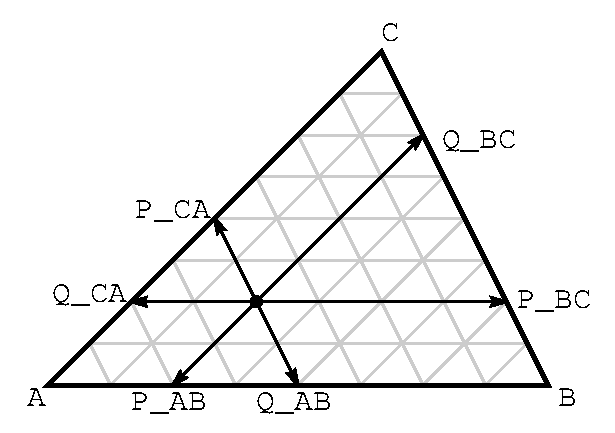
\includegraphics[width=75mm]{fig-triangle.eps}} }

The coefficients for the interpolation have simpler formulas when compared with the ones in the
constructor of a rectangle (presented in paragraph \numb section 10.\numb parag 3);
the fact that we interpolate from six vertices compensates that.

Examples are presented in paragraphs \numb section 1.\numb parag 4, \numb section 1.\numb parag 5
and \numb section 2.\numb parag 5
\vfil\eject

\paragraph{\numb section 10.\numb parag 5. Progressive mesh generation}

Constructor {\codett Mesh::Mesh ( tag::progressive, ... )}, declared in {\codett mesh.h} and defined
in {\codett progressive.cpp}, builds a mesh on a given manifold starting with almost nothing.
More precisely, it starts with the boundary of the future mesh, then it
moves this interface with small steps, building the mesh behind it like a spider.
Actually, if the manifold is compact (like the sphere or the torus) and we want to mesh all of it,
there will be no boundary.
In this case we can start the process by providing nothing more than the manifold itself.
Section \numb section 3 gives several examples.

This is a complex process, much more complex than building a regular mesh of rectangles
(as described in paragraph \numb section 10.\numb parag 3) or of triangles (as described
in paragraph \numb section 10.\numb parag 4).
The constructor delegates the job to the function {\codett progressive\_construct}.

The mesh must follow the shape of the manifold; this is achieved by {\codett project}ing
newly created vertices on the working manifold.

The initial interface may be disconnected.
Even if the initial interface is connected, it may become disconnected during the meshing
process, if it touches itself (paragraph \numb section 10.\numb parag 8 discusses this event).

Detecting such touching points requires evaluating the distance between many pairs of points.
This may become extremely time consuming, unless special care is taken to organize points
belonging to the interface in a hierarchy allowing one to eliminate many pairs of points
from the evaluation process.
Paragraph \numb section 9.\numb parag 15 describes this hierarchy.

The next few paragraphs describe specific parts of this process of progressive mesh generation.


\paragraph{\numb section 10.\numb parag 6. The normals}

The meshing process described in paragraph \numb section 10.\numb parag 5 uses a set of
normal vectors.
Each segment in the interface has associated to it
a vector tangent to the working manifold and normal to the interface (we can
think of the interface as a curve embedded in that two-dimensional manifold).
These normal vectors provide the sense in which we want the mesh to grow (to the left or to
the right of the interface), that is, they define the orientation of the manifold and of
the mesh under construction.
They are used when we create a new vertex in order to decide its placement.

Actually, at the beginning of the process only one segment has an associated normal vector.
{\ManiFEM} then propagates this normal vector to the neighbour segments, walking along
the current connected component of the interface.
This means that, if there are other connected components, they will have no normal vectors.
When the current connected component of the interface touches other connected components
(this event is discussed in paragraph \numb section 10.\numb parag 8), {\maniFEM}
% aproveita a oportunidade para ...
propagates the normal vectors to the new connected component.

Each time a new segment is added to the interface (this happens in situations described in
paragraphs \numb section 10.\numb parag 7 and \numb section 10.\numb parag 8),
the normal associated to the new segment must be computed (propagated from neighbour
segments).
\vfil\eject


\paragraph{\numb section 10.\numb parag 7. Filling triangles}

Perhaps the simplest part of the meshing process described in paragraph
\numb section 10.\numb parag 5 is just walking along the interface and adding new triangles.

A trivial case is when an angle is encountered which is close to $ 60^\circ $
(see figure below left).
Then we only have to fill the space with a new triangle.
Of course, before creating this new triangle a new segment {\codett AB} must be created
(no new vertex is needed).
Two old segments must be removed from the interface and the new one must be added.
Its normal must be computed (see paragraph \numb section 10.\numb parag 6).

{ \psfrag{A}{\special{ps: gsave 0 0 0.8 setrgbcolor}{\codett A}\special{ps: grestore}}
  \psfrag{B}{\special{ps: gsave 0 0 0.8 setrgbcolor}{\codett B}\special{ps: grestore}}
  \psfrag{P}{\special{ps: gsave 0 0 0.8 setrgbcolor}{\codett P}\special{ps: grestore}}
  \psfrag{point60}{\special{ps: gsave 0 0 0.8 setrgbcolor}
    {\codett point\_60}\special{ps: grestore}}
  \psfrag{point120}{\special{ps: gsave 0 0 0.8 setrgbcolor}
    {\codett point\_120}\special{ps: grestore}}
  \centerline{\includegraphics[width=45mm]{fill-angle-60.eps}
  \hskip5mm \includegraphics[width=45mm]{fill-angle-120.eps}} }

A more complicated situation is when an angle is encountered which is close to $ 120^\circ $
(see figure above right).
A new vertex {\codett P} is created; its position is defined based on the two normals
of the adjacent segments.
Two new segments {\codett AP} and {\codett BP} are created,
then two new triangles are created and added to the mesh under construction.
Two old segments are removed from the interface then {\codett AP} and {\codett BP} are added
to the interface (their normals must be computed).

Special situations must be dealt with.
For instance, if one or both neighbour angles are also close to $ 120^\circ $,
we must take more vertices into account when we place the newly created vertex {\codett P};
figure below shows such situations.

  \centerline{\includegraphics[width=45mm]{fill-angle-120-a.eps}
  \hskip5mm \includegraphics[width=40mm]{fill-angle-120-b.eps}}

Finally, if all angles of the current connected component of the interface are wide,
we may want to create a triangle ``out of the blue'', like in figure below.

\centerline{\includegraphics[width=32mm]{fill-blue.eps}}

Every time a new vertex is created, we must check whether it came close to another
zone of the interface and take action as described in paragraph \numb section 10.\numb parag 8.


\paragraph{\numb section 10.\numb parag 8. Touching the interface}

During the meshing process described in paragraph \numb section 10.\numb parag 5,
distinct zones of the moving interface may
come close to each other and the algorithm will eventually put them in contact.
Figure below shows the situation just prior to the contact.
The two zones may belong to different connected components of the interface,
as in the configuration shown below on the left.
In this case, the two components will merge, producing a new chain.
The normal vectors will be propagated to the segments which did not have an associated
normal vector (see paragraph \numb section 10.\numb parag 6).
But it may also happen that they are part of the same connected component,
see the drawing below on the right.
In this case, the current chain will split in two.

\centerline{\includegraphics[width=5cm]{touching-interf-1.eps}
\hskip5mm \includegraphics[width=5cm]{touching-interf-2.eps}}

Methods {\codett glue\_two\_segs\_S} and
{\codett glue\_two\_segs\_Z} deal with two possible ways in which two
zones of the interface may touch,
independently of whether the two zones belong to the same connected component or not.
In the drawing below on the right hand side an S-shaped connection is created,
while in the other drawing a Z-shaped connection is created.


{ \psfrag{A}{\special{ps: gsave 0 0 0.8 setrgbcolor}{\codett A}\special{ps: grestore}}
  \psfrag{B}{\special{ps: gsave 0 0 0.8 setrgbcolor}{\codett B}\special{ps: grestore}}
  \psfrag{C}{\special{ps: gsave 0 0 0.8 setrgbcolor}{\codett C}\special{ps: grestore}}
  \psfrag{D}{\special{ps: gsave 0 0 0.8 setrgbcolor}{\codett D}\special{ps: grestore}}
  \centerline{\includegraphics[width=32mm]{connect-S.eps}
  \hskip10mm \includegraphics[width=55mm]{connect-Z.eps}} }


%%%%%%%%%%%%%%%%%%%%%%%%%%%%%%%%%%%%%%%%%%%%%%%%%%%%%%%%%%%%%%%%%%%%%%%%%%%%%%%%%%%%%%%%%%%%%%%
%%%%%%%%%%%%%%%%%%%%%%%%%%%%%%%%%%%%%%%%%%%%%%%%%%%%%%%%%%%%%%%%%%%%%%%%%%%%%%%%%%%%%%%%%%%%%%%


\section{Index}

boundary of a cell : \numb section 1.\numb parag 2, \numb section 8.\numb parag 3

cell : \numb section 1.\numb parag 2, \numb section 8.\numb parag 1

cloud : see {\codett MetricTree}

dimension of a cell or mesh : \numb section 1.\numb parag 2, \numb section 9.\numb parag 3,
\numb section 9.\numb parag 5

discarding a mesh : \numb section 9.\numb parag 7

docking (of a finite element on a cell) : \numb section 7.\numb parag 2

errors : \numb section 9.\numb parag 11, \numb section 9.\numb parag 12

{\codett Field} : \numb section 6.\numb parag 1

factory functions : \numb section 9.\numb parag 3

{\codett Function} : \numb section 6.\numb parag 1

interpolation of coordinates : \numb section 2.\numb parag 3 -- \numb section 2.\numb parag 9,
\numb section 10.\numb parag 2 -- \numb section 10.\numb parag 4

iterators over cells : \numb section 8.\numb parag 5, \numb section 8.\numb parag 7

{\codett init\_cell} : \numb section 9.\numb parag 8

{\codett join}ing meshes : \numb section 1.\numb parag 3, \numb section 1.\numb parag 4,
\numb section 1.\numb parag 5, \numb section 2.\numb parag 1, \numb section 2.\numb parag 2,
\numb section 2.\numb parag 4, \numb section 2.\numb parag 5, \numb section 2.\numb parag 6,
\numb section 8.\numb parag 2

level set : see manifold, defined by an implicit equation

m-tree : \numb section 9.\numb parag 15

manifold, Euclidian : all over the place\hfil\break
\hglue 15mm (any code using {\maniFEM} must begin by declaring a Euclidian manifold)

manifold, defined by an implicit equation : \numb section 2.\numb parag 4 --
\numb section 2.\numb parag 9, section \numb section 3

manifold, parametric : \numb section 2.\numb parag 12, \numb section 2.\numb parag 13

manifold, quotient : section \numb section 5

mesh : all over the place, esp.\ \numb section 1.\numb parag 2, \numb section 1.\numb parag 3,
\numb section 8.\numb parag 1, \numb section 8.\numb parag 3, \numb section 8.\numb parag 7
-- \numb section 8.\numb parag 10

{\codett MetricTree} : \numb section 9.\numb parag 15, \numb section 9.\numb parag 16

negative {\codett Cell} or {\codett Mesh} : see orientation of {\codett Cell}s and
{\codett Mesh}es

oct-tree : \numb section 9.\numb parag 15

orientation of {\codett Cell}s and {\codett Mesh}es : \numb section 1.\numb parag 2,
\numb section 1.\numb parag 3, \numb section 8.\numb parag 1, \numb section 8.\numb parag 7,
\numb section 9.\numb parag 6

orientation of a {\codett Manifold} : \numb section 3.\numb parag 10

parametric manifold : see manifold, parametric

progressive mesh generation : section \numb section 3, \numb section 9.\numb parag 16,
\numb section 10.\numb parag 5 -- \numb section 10.\numb parag 8

projection, onto a manifold : \numb section 2.\numb parag 3 -- \numb section 2.\numb parag 9

quad-tree : \numb section 9.\numb parag 15

quotient manifold : see manifold, quotient

reverse cell or mesh : see orientation of cells and meshes

segment {\codett Cell}s : \numb section 1.\numb parag 2

segment {\codett Mesh}es : \numb section 1.\numb parag 1 -- \numb section 1.\numb parag 3,
\numb section 9.\numb parag 14

{\codett set\_as\_working\_manifold} : \numb section 2.\numb parag 8,
\numb section 2.\numb parag 9, \numb section 2.\numb parag 11, \numb section 3.\numb parag 1,
\numb section 3.\numb parag 2, \numb section 3.\numb parag 3, \numb section 3.\numb parag 9,
\numb section 3.\numb parag 14 -- \numb section 3.\numb parag 24

{\codett tag}s : \numb section 9.\numb parag 2




\bye

%%%%%%%%%%%%%%%%%%%%%%%%%%%%%%%%%%%%%%%%%%%%%%%%%%%%%%%%%%%%%%%%%%%%%%%%%%%%%%%%%%%%%%%%%%%%%%%

\hbox{\includegraphics[width=19mm]{manifem-small.eps}}


The factory function {\codett FE\_function::from\_string} accepts expressions like {\codett "x+y+z"} or
{\codett "x\^{}3-.22E-4*y\^{}2+5.4"} (which stands for $ x^3 - 0.0000022y^2+5.4$) 
but not expressions involving parentheses.

There are other ways of building symbolic expressions.
For example,

\verbatim
   auto fx = FE_function::from_string ( "x" ); // FE_function * fx
   auto fy = FE_function::from_string ( "y" );
   auto five = FE_function::constant (5); // FE_function * five
   auto s = FE_function::sum (fx,fy,five); // FE_function * s
   auto p = FE_function::power (s,3); // FE_function * p, or
   // p = (x+y+5)^3
\endverbatim

\noindent or

\verbatim
double ff(double x, double y) { return sin(x)*cos(y); }
int main () {
   auto f = FE_function::function (ff); // FE_function * f
}\endverbatim















